\documentclass{template}
\usepackage{graphicx,parskip,bibunits,appendix,float}
\usepackage[ruled] {algorithm2e}
\usepackage{url,amsmath,amssymb,fancybox,listings,pdfpages,caption,multicol,multirow,datetime,rotating, booktabs}
%\usepackage[usenames,dvipsnames]{color}
\usepackage[pagebackref=false,pdffitwindow=true]{hyperref}
\usepackage[acronym]{glossaries}

\usepackage[export]{adjustbox} %To adjust images
\usepackage{multirow}

%NOTE: The hyperref usepackage should be the last \usepackage!!
%NOTE: When pagebackref=true an error will appear at the end of compiling. press `q' to ignore
%NOTE: Referencing Algorithms does not work if this usepackage is before the hyperref include.!!
%NOTE: This is a comment, ignored when the document is compiled
%NOTE: The following document configuration settings generally do not need to be modified
%NOTE: More packages may need to be added to provide additional functionality

\hypersetup{
    pdftitle    = {CAWIML: A Computer Assisted Web Interviewing Mark-up Language},
    pdfauthor   = {Jose Lloret},
    pdfsubject  = {Computing},
    pdfkeywords = {survey, questionnaire, xml, mark-up, xml schema, xml language, cai, cawi, rest, single-page},
    colorlinks  = true, anchorcolor = blue, filecolor = blue, urlcolor = blue,
    linkcolor   = blue,    %NOTE: change (blue) to (colIdentifier) to have links within the document in Black
    citecolor   = blue,    %NOTE: change (blue) to (colIdentifier) to have citation links within the document in Black
}

\definecolor{colBackGrnd}{rgb}{1,1,0.8}
\definecolor{colKeys}{rgb}{0,0,1}
\definecolor{colIdentifier}{rgb}{0,0,0}
\definecolor{colComments}{rgb}{0,.5,0}
\definecolor{colString}{rgb}{0,0,1}
\definecolor{colWhite}{rgb}{1,1,1}

\newcommand{\MyHookSign}{\hbox{\ensuremath\hookleftarrow}}

\newtheorem{Theorem}{Theorem}
\newtheorem{Proposition}[Theorem]{Proposition}
\newtheorem{Lemma}[Theorem]{Lemma}
\newtheorem{Proof}[Theorem]{Proof}
\newtheorem{Remark}[Theorem]{Remark}
\newtheorem{Claim}[Theorem]{Claim}
\newtheorem{Example}[Theorem]{Example}
\newtheorem{Definition}[Theorem]{Definition}

%NOTE: Setup for including program listings
\lstset{%
    float=H,
    basicstyle=\ttfamily\footnotesize,
    identifierstyle=\color{colIdentifier},
    keywordstyle=\color{colIdentifier}, %
    stringstyle=\color{colIdentifier},
    commentstyle=\color{colIdentifier}, %
    columns=flexible,
    tabsize=2,
    frame=single,
    extendedchars=true, %
    showspaces=false,
    showstringspaces=false,
    numbers=left, %
    numberstyle=\footnotesize,
    breaklines=true,
    prebreak={\space\MyHookSign},
    language=Java,
    backgroundcolor=\color{colBackGrnd},
    breakautoindent=true, %
    captionpos=b%
} %\hypersetup{colorlinks=true, citecolor=\color{colIdentifier}}

\sloppy %NOTE: To ensure the Right Hand Margin is used (Especially for long URLS)
%NOTE: END of the document configuration settings

\begin{document}

\DeclareGraphicsExtensions{.tiff,.jpg,.png,.gif,.pdf}
%NOTE: When inserting Figures if the extension of the graphic file is not provided LaTeX will automatically search
% for the extensions declared above, in the order declared.

\title{\huge{CAWIML: A Computer Assisted Web Interviewing Mark-up Language}}
\author{Jose Miguel Lloret Perez}
\degreetitle{Master of Research} % Replace with appropriate degree
\rpttype{MRes}    % Replace MSc with BSc for Honours Degree Year projects.
\principaladviser{Dr. Nirmalie Wiratunga}

\newacronym{xml}{XML}{Extensible Markup Language}
\newacronym{dsl}{DSL}{Domain Specific Language}
\newacronym{html}{HTML}{HyperText Markup Language}
\newacronym{css}{CSS}{Cascading Style Sheets}
\newacronym{xhtml}{XHTML}{Extensible HyperText Markup Language}
\newacronym{http}{HTTP}{Hypertext Transfer Protocol}
\newacronym{cai}{CAI}{Computer-Assisted Interviewing}
\newacronym{cati}{CATI}{Computer-Assisted Telephone Interviewing}
\newacronym{capi}{CAPI}{Computer-Assisted Personal Interviewing}
\newacronym{casi}{CASI}{Computer-Assisted Self Interviewing}
\newacronym{cawi}{CAWI}{Computer-Assisted Web Interviewing}
\newacronym{ktp}{KTP}{Knowledge Transfer Partnerships}
\newacronym{csm}{CSM}{Computer-assisted Survey methods}
\newacronym{csv}{CSV}{Comma-separated Values}
\newacronym{spss}{SPSS}{Statistical Package for the Social Sciences}
\newacronym{cases}{CASES}{Computer-Assisted Survey Execution System}
\newacronym{dtd}{DTD}{Document Type Definition}
\newacronym{xsd}{XSD}{XML Schema Definition}
\newacronym{relaxng}{RELAX NG}{Regular Expression Language for XML New Generation}
\newacronym{sch}{SCH}{Schematron}
\newacronym{triples}{Triple-S}{Survey Interchange Standard}
\newacronym{qdl}{QDL}{Questionnaire Definition Language}
\newacronym{tadeq}{TADEQ}{Tool for Analysis and Documentation of Electronic Questionnaires}
\newacronym{sss}{SSS}{Simple Survey System}
\newacronym{rti}{RTI}{Research Triangle Institute}
\newacronym{abs}{ABS}{Austrian Bureau of Statistics}
\newacronym{insee}{INSEE}{National Institute of Statistics and Economics Studies}
\newacronym{pof}{POF}{Proof of Concept}
\newacronym{sqbl}{SQBL}{Structured Questionnaire Building Language}
\newacronym{ddi}{DDI}{Data Documentation Initiative}
\newacronym{ssm}{SSM}{Survey State Model}
\newacronym{cawiml}{CAWIML}{Computer Assisted Web Interviewing Markup Language}
\newacronym{efsm}{EFSM}{Extended Finite State Machine}
\newacronym{pn}{PN}{Polish Notation}
\newacronym{rpn}{RPN}{Reverse Polish Notation}
\newacronym{iso}{ISO}{International Organization for Standardization}
\newacronym{iec}{IEC}{International Electrotechnical Commission}
\newacronym{json}{JSON}{JavaScript Object Notation}
\newacronym{icpsr}{ICPSR}{Inter-university Consortium for Political and Social Research}
\newacronym{poc}{POC}{Proof of Concept}
\newacronym{rti}{RTI}{Research Triangle Institute}
\newacronym{cs}{CS}{Client-Server}
\newacronym{rest}{REST}{Representational State Transfer}
\newacronym{dal}{DAL}{Data Access Layer}
\newacronym{nosql}{NoSQL}{No Structured Query Language}
\newacronym{mvc}{MVC}{Model-View-Controller}
\newacronym{asp}{ASP}{Active Server Pages}
\newacronym{saas}{SaaS}{Software as a Service}
\newacronym{soa}{SOA}{Service Oriented Architecture}
\newacronym{dom}{DOM}{Document Object Model}
\newacronym{w3c}{W3C}{World Wide Web Consortium}
\newacronym{xslt}{XSLT}{Extensible Stylesheet Language Transformations}
\newacronym{api}{API}{Application Program Interface}
\newacronym{dsdl}{DSDL}{Document Schema Definition Languages}
\newacronym{soap}{SOAP}{Simple Object Access Protocol}
\newacronym{corba}{CORBA}{Common Object Request Broker Architecture}
\newacronym{wcf}{WCF}{Windows Communication Foundation}
\newacronym{ajax}{AJAX}{Asynchronous JavaScript and XML}
\newacronym{spa}{SPA}{Single Page Application}
\newacronym{uri}{URI}{Uniform Resource Identifier}
\newacronym{url}{URL}{Uniform Resource Locator}
\newacronym{jaxrs}{JAX-RS}{Java API for RESTful Web Services}
\newacronym{cbr}{CBR}{Case-based Reasoning}
\newacronym{www}{WWW}{World Wide Web}
\newacronym{oasis}{OASIS}{Organization for the Advancement of Structured Information Standards}
\newacronym{wsgi}{WSGI}{Web Server Gateway Interface}
\newacronym{ssl}{SSL}{Secure Socket Layer}
\newacronym{ipsec}{IPsec}{Internet Protocol Security}


\beforeabstract
\newpage
\prefacesection{Abstract}
		\gls{cawi} is the new mode of conducting surveys through web browsers. This on-line solution extends the traditional paper questionnaire with functionality to inform the order of questions, the logic to guide question relevance and inconsistency checks to validate responses. Large scale international surveys are typically conducted by research agencies in multiple countries using \gls{cawi} systems. However, these demand for non-proprietary and platform independent questionnaire definitions that work throughout multiple survey systems.

	In this thesis, we conduct a comparative analysis at two levels: one for the different \gls{xml} authoring solutions that capture questionnaire features; and another to explore the architecture styles for the most popular \gls{cawi} solutions. The popular hierarchical model, employed to manage the questionnaire flow, is not semantically intuitive to domain experts and lacks flexibility to allow for questionnaire design refinements. An analysis of system architectures suggests that the commonly adopted multi-page paradigm to build web pages, neither reduces the server burden nor addresses the responsiveness requirements expected from survey systems.

	Accordingly to address the language shortcomings we introduce a \gls{cawiml} that uses two schema languages to validate vocabulary, structures and relationships among \gls{xml} constructs and adopts a state-transition model to manage the routing and flow of questions. \gls{cawiml} serves our \gls{rest} system to drive the design and collection stages through a single-page web build. We present our language results from testing \gls{cawiml} on a comprehensive set of real-world surveys from Pexel Research Services and use the distribution of \gls{cawiml}'s vocabulary on this sample to demonstrate its coverage of questionnaire features and effective routing support. In order to evaluate our platform, we computationally simulate both the stress test for parallel processing of requests and interviewee behaviour in terms of different user interaction response configuration levels. Results suggest that both the parallelism and variation in user behaviour can be handled within acceptable levels of usability thresholds.

	\textbf{Keywords:} survey, questionnaire, xml, mark-up, xml schema, cai, cawi, state-transition, rest, single-page.
	%We present our language results from testing \gls{cawiml} on a comprehensive set of real-world surveys from Pexel Research Services and evaluate our platform at different configuration levels of concurrency considering response time usability thresholds.
\prefacesection{Declaration of Authorship}
		I declare that I am the sole author of this thesis and that all verbatim extracts contained in the thesis have been identified as such and all sources of information have been specifically acknowledged in the bibliography. Parts of the work presented in this thesis have appeared in the following publication:

	\begin{itemize}
		\item Lloret, J. and Wiratunga, N. (2015). Survey state model (SSM). XML Authoring of Electronic Questionnaires. In XML Prague. A conference on XML, pages 159-177. (Chapter \ref{ch:cawiLanguage})
	\end{itemize}
\prefacesection{Acknowledgements}
		Firstly, I would like to express my sincere gratitude to my supervisor Dr. Nirmalie Wiratunga for the continuous support of my MRes study and related research, for her patience, motivation, and immense knowledge. Her guidance has helped me in all the time of research and writing of this thesis.

	Besides my supervisor, I would like to thank Pexel Research Services and Robert Gordon University for giving me the opportunity to undertake a \gls{ktp} project with the possibility to study for a postgraduate qualification. In particular, I am grateful to Bruce Leslie for his insightful comments and expertise at every stage of this research, but also for his task of selecting and testing the real-world survey samples through my experiments.

	On a more personal level, I must thank my patient and understanding girlfriend Daria for all her love and support. She has not only accepted me on all my bad days but also has encouraged me many times to put all my best for this research. I have also to mention perhaps the most faithful companion, my dog Hugo, for all the days and nights that he has been sat next to me.

	Last but not least, I thank my family, and in particular my mum, who has been always proud of all the efforts I have made in order to look for better career opportunities.

	
\glsresetall

\afterpreface 

\afterabstract
%\listofalgorithms   %NOTE: Will generate a list of Algorithms in the Table of Contents Section
%\lstlistoflistings  %NOTE: Will generate a list of Program Listings in the Table of Contents Section

%NOTE: Include the relative reference for each chapter to be included
% dividing the thesis file structure into a number of directories aids development
% format: directoryName/filename (the .tex extension is not required for the filename)

\chapter{Introduction}\label{ch:introduction}
\pagenumbering{arabic} \setcounter{page}{1}
		This Chapter presents \gls{cawiml} as an alternative authoring language to specify questionnaires only using standard \gls{xml} schema languages. Particularly, it uses a state-transition paradigm for question's sequence and is intended to facilitate the questionnaire routing logic more adequately than the popular hierarchical model. \gls{rpn}, is the expression formalism utilised for describing routing and personalisation constructs indistinctly.

	The rest of this Chapter is structured as follows: Section \ref{sec:cawiLanguage:stateTransition} introduces the state-transition routing structure. Section \ref{sec:cawiLanguage:rpn} explains the postfix notation mode as the formalism for questionnaire expressions, followed by Section \ref{sec:cawiLanguage:xmlLanguage} that explains our \gls{xml} authoring solution. Finally, \gls{xml} details for content, routing and personalisation constructs expressed in \gls{cawiml} are presented in Section \ref{sec:cawiLanguage:cawiml}.
	\section{Research Motivation}
			The \emph{correctness} of a questionnaire specification involves two tasks: one is checking that every construct conforms to a vocabulary, structure and content, i.e. the grammatical aspect, and the other consist of validating integrity relations and business specific constraints, i.e. the validation rules. Authoring language solutions such as Blaise and \gls{cases} sufficiently address both levels of correctness, however the problem arises when large surveys (e.g. European Community Household Panel, European Union Labour Force Survey or European Health Interview Survey among others) have to be conducted through several research agencies across different countries. Since these companies usually have different \gls{cai} solutions to support the life-cycle of survey research, the use of specifications that are only understandable by specific software solutions, raises the need for having a language solution that is \emph{non-proprietary} and \emph{platform independent}.

	Two exchangeable data formats exist today to address the requirements of reusable questionnaire specifications: one is \gls{xml}, widely used to exchange data among organisations and best known for its declarative and extensible properties; and the other is \gls{json}, increasingly used to communicate modern web applications because of its direct support by JavaScript. Intuitively, the \gls{json} choice is more attractive due to its less verbose expressive descriptions as well as its faster performance when compared to \gls{xml} \cite{art:nurseitov09}. However, it lacks support from standards such as \gls{w3c} or \gls{iso} in terms of including rules that can validate correctness of documents. Accordingly for this research we make use of XML as an authoring solution making use of its different schema solutions to express constraints. %What do you mean here by constraints? do you mean constructs?

	The \emph{routing structure} of a questionnaire is another aspect that has to be carefully considered. When the flow of a questionnaire is defined, designers or social researchers commonly use skip patterns to filter one or several questions. This enables the smooth movement from one part of the questionnaire to another by removing irrelevant questions from an interview. Despite the fact that using unstructured patterns such as GOTO to express logic in programming was stated by Djisktra \cite{art:dijkstra68}, it is widely accepted by the software community as best avoided. In contrast, social researchers, who are typically the designers of questionnaires, have no qualms about designing questionnaires with complex logic that involve multiple GOTO constructs. Therefore, a solution to find a modelling structure that describes questionnaires in a structured manner while allowing designers to express their logic without the need for programmers is needed \cite{masterthesis:madsen09}.

	In addition to the issues related to the specification of questionnaires, there exists different architectural properties that should also be considered when designing a \gls{cawi} solution:
	\begin{itemize}
		\item \emph{Scalability}, known as the capacity to work under different workloads. For instance, when an interview is carried out, keeping the status of the last operation performed for each respondent is needed. As such, this is typically solved by storing interviewee's status through a session variable making it impossible to free server resources until an interview is completed. This stateful communication impacts negatively over the infrastructure making it hard to replicate and synchronise an architecture when multiple servers can handle requests from the same respondent.
		\item \emph{Simplicity}, which is achieved through the separation of functionalities such as the user interfaces into a separated component within the server \cite{phdthesis:fielding00}. For instance, popular \gls{cawi} solutions such as SurveyMonkey use the \gls{mvc} design pattern for building multiple web pages on the server. However, with the introduction of the second generation of \gls{www}, these tasks can be moved to the client, i.e the browser, and help to reduce not only the time to complete requests but also simplify the server burden.
		\item \emph{Portability}, that permits a software solution running on different platforms. This architectural property has particular significance for web application allocation where it is important to frequently utilise services from large data centres. For that purpose, it is not desired that a \gls{cawi} solution is tied to a particular operating system or more specifically to have a database solution that is platform dependent.
		\item \emph{Reliability}, which is determined by the capacity of a system to replace a component under any failure. This property constitutes one of the most important aspects to consider since a \gls{cawi} system has to offer flexibility to allow questionnaire completion when it suits the user. 
	\end{itemize}
	
	In order to address the issues discussed above in relation to the specification of questionnaires as well as the architectural properties of \gls{cawi} systems, this thesis explores the following research questions:

	\begin{enumerate}
		\item Are the current state-of-art \gls{xml} authoring languages able to validate the correctness of questionnaire constructs using standard \gls{xml} schema languages?
		\item How can we represent the flow of questionnaires using structured patterns adapted to facilitate the questionnaire logic for routing purposes? %I removed the reference to designers, in case they ask us to evaluate it with designer feedback!
		\item Do the popular \gls{cawi} solutions consider the architectural properties of scalability, flexibility, portability and reliability adequately?
	\end{enumerate}
	\section{Research Aim and Objectives}
			The aim of this thesis is to design and implement a new \gls{cawi} solution that provides web interfaces closer to native desktop applications. Specifically, this study is focused on the design and collection stages of surveys but also extends its functionality to cover some aspects of the management, analysis and reporting stages. The system solution has to have a clear separation of concerns, i.e. an authoring \gls{xml} solution should be utilised to create questionnaire specifications through a visual design interface and similarly these descriptions should aid to automatically drive the routing logic for survey response data collection.

	%Since this thesis is focused on the development of a web application, it is expected that the architectural design adheres to properties such as \emph{scalability}, \emph{simplicity}, \emph{portability} and \emph{reliability}. Additionally, as our aspiration is to create a commercial advantage, we expect that the combination of a novel architecture, \gls{xml} language and responsive interfaces will form important contributions to applied research in \gls{cawi} systems.

	As such, we intend to achieve our research aim with the following six objectives:

	\begin{enumerate}
		\item Conduct a comparative analysis of the state-of-art \gls{xml} language solutions that cover questionnaire definitions with a focus on the coverage of constructs and the capacity to validate correctness with standard \gls{xml} schema formalisms.
		\item Critically appraise current modelling approaches in terms of their ability to manage questionnaire flow definitions for the purposes of routing.
		\item Develop a new \gls{xml} authoring solution to better address the correctness, together with the state-transition structures necessary for routing.
		\item Analyse the architecture of different \gls{cawi} solutions in order to determine whether the necessary and sufficient properties for a \gls{cawi} system solution are induced or not. 
		\item Implement an architecture based on \gls{rest} to better handle architectural properties such as scalability, simplicity, portability or reliability.
		\item Conduct an evaluation at two levels, one for the coverage of questionnaire constructs and another to evaluate the capacity of the proposed architecture to work under different workloads.
	\end{enumerate}
	\section{Significance of Research Contributions}
			This study has been carried out as part of the \gls{ktp} project between Robert Gordon University and Pexel Research Services \footnote{\url{http://www.pexel.co.uk/}}. This company, which is based on Glasgow, conducts telephone interviewing through its own infrastructure of units and is considered one of the largest in Europe. With the emergence of the new on-line survey mode, they are keen to consider the design and development of a new hybrid solution that permits cost reductions of training their staff to use complex interfaces.

	The first significant contribution of this work has been to design a novel \gls{xml} solution that combines two approaches for expressing constraints in \gls{xml}. The validation of correctness, conducted in a two-step process, permits reducing or eliminating the need to rely on general purpose programming languages for checking complex rules. Moreover, as the \gls{xml} language proposes the state-transition paradigm to express questionnaire's routing, not only is it better able to adapt to changes in specifications but also the use of structured patterns allows for adaptability that can support and mimic the requirements that are important to designers of questionnaires (such as social researchers).

	The second significant contribution has been the system architecture that better induces the properties of: scalability, through a stateless communication among the parts; simplicity, by transferring the web pages building to the client-side; portability, through a platform independent programming language combined with a cross platform database choice; and reliability, through loose coupling components that are easy to change under any failure.

	Secondary contributions of this research include the possibility to incorporate a searchable central repository of survey definitions according to our \gls{xml} solution. This has the potential to help researchers, who often want to know what questions can be used for a particular topic \cite{proc:corbett11}, to reuse past questions when creating new questionnaires.
	\section{Ethical Issues}
			The \gls{xml} solution that we have designed has been evaluated against several real questionnaires provided by third parties to Pexel. These paper questionnaires remain under the company premises and cannot be disclosed. In the Appendix \ref{sec:appendix:questionnaires}, we have provided links to these real questionnaires implemented in our authoring language, however, we have replaced and eliminated any sensitive information in order to anonymise the third parties behind each survey. In respect to the survey used to explain the different features that a questionnaire may have (see Figure \ref{fig:background:survey}), this instance constitutes a simulated paper questionnaire and consequently does not contain any confidential information from any third party.

	The evaluation of our new \gls{cawi} architecture for the gathering of responses for questionnaires presented in Chapter \ref{ch:evaluation} has used randomly generated data, thus having no ethical implications. Other experiments that have been conducted during the course of this on-line survey solution such as usability testing in which the system was evaluated by Pexel's employees, may contain personal details or handling of commercially sensitive information but these are adequately described by \gls{iso} 20252 with which the company complies.

	\section{Thesis Overview}
			The rest of this thesis is outlined as follows: Chapter \ref{ch:background} introduces the different questionnaire features that can be used to specify surveys. We also discuss \gls{xml} as the exchangeable data format to create reusable questionnaire definitions together with an extensive comparison of the relevant \gls{xml} schema languages to validate and check correctness at grammatical and semantic levels.

	In Chapter \ref{ch:literature} we conduct a comparative analysis of the state-of-art \gls{xml} languages for questionnaire design with focus on routing and personalisation aspects, notation adopted to define questionnaire expressions, schema language utilised to define constraints as well as flow modelling for question's sequencing. Additionally, we explore different architecture styles adopted by the most relevant \gls{cawi} systems in order to determine how well they support properties such as scalability, simplicity, portability and reliability.

	Chapter \ref{ch:cawiLanguage} presents the \gls{cawiml}, a contribution of this thesis to address the validation of questionnaire specifications using \gls{xml} schema formalisms. Here we explain the state-transition paradigm adopted to model questionnaire flow and present the \gls{rpn} notation formalism to define expressions that permit filtering, computing or personalising questions and their contents. The use of \gls{cawiml}'s main features are discussed using a running example of a questionnaire.

	Chapter \ref{ch:cawiSystem} presents a \gls{rest} based architectural solution that implements the expected \gls{cawi} system properties. Different layers for communicating client and server, the business objects that address the survey life-cycle stages as well as its non-relational persistence solution to address high demands of data are presented. Additionally, the \gls{spa} paradigm adopted to build the client interfaces directly in browsers is discussed.

	Evaluation is in Chapter \ref{ch:evaluation} with results organised under two themes: coverage of questionnaire constructs by \gls{cawiml} analysed on fifteen real questionnaires; and simulated load testing of increasing numbers of concurrent users with focus on different response time thresholds.

	We conclude this thesis in Chapter \ref{ch:Conclusion} with a summary of our main contributions and desirable extensions for future work.
\chapter{Background}\label{ch:background}
	This chapter is intended to introduce the reader to the terminology and concepts in the context of \gls{cai} systems. We have focused our efforts on \gls{xml} as the standard for exchange and representation of electronic questionnaires. Although we could have considered \gls{json} as a more attractive representation format due to its direct mapping to JavaScript objects, its simplicity and its less verbosity for using across a web application, we have discarded it because as far as we know, there is no standard schema formalism that permits the validation of correctness without relying on general purpose programming languages.

	The rest of this Chapter is structured as follows: Section \ref{sec:background:questionnaires} uses an example questionnaire to describe the different features that are used in surveys. The Section \ref{sec:background:xml} explains the origin of \gls{xml} as well as the requirements needed to consider a file as \gls{xml} well-formed. Section \ref{sec:background:xmlSchemas} discusses the different schema paradigms that can be used to create constraints over well-formed \gls{xml} documents and finally, Section \ref{sec:background:xPath} introduces the reader to XPath query language since it is widely used for specifying sophisticated constraints.

\section{Electronic Questionnaires}\label{sec:background:questionnaires}
		Questionnaires are defined as instruments to collect data. Typically, they are composed of questions and instructions to guide the flow through an interview. With the introduction of \gls{cai} systems, these have been extended with additional features. There are two studies that explore the different constructs required to specify questionnaires. The first approach, proposed by Katz \cite{proc:katz97}, describes the different tasks involved in creating specifications for questionnaires whereas the second proposal, introduced by Bethlehem \cite{proc:bethlehem00}, uses an object-oriented paradigm to better understand all the features of an electronic questionnaire.

	In order to describe all the different constructs that may be used to construct questionnaires, we present in Figure \ref{fig:background:survey} a questionnaire intended to unify the efforts from Katz and Bethlehem. The most common types of questions are \emph{single-response}, \emph{multiple-response} and \emph{open-ended} (e.g. Q1, Q3 and Q5 respectively) whilst \emph{grid} (e.g. Q4) unlike the common types is naturally more cognitively demanding on the interviewee since more than one question in the form of rows is asked \cite{web:bock13}.

	Usually questionnaires are divided into \emph{sections} where \emph{intro} statements (e.g. INF1, INF2, END) become helpful to establish the context and introduction to a part of the questionnaire. For instance, in this example, there are two sections used to organise the set of questions, the outer section for INF1, Q1, Q2, Q3, Q4, Q5, INF2 and END and an inner for Q6a which can be asked multiple times. 

	The \emph{instructions}, in bold font, are normally included to manage questionnaire routing according to interviewee responses. There are three such routing constructs describing the flow through the questionnaire in our example:

	\begin{itemize}
		\item \emph{skip} feature allows the interviewee to skip over questions to move on to another question. This can be an \emph{unconditional} skip, as in the case of skips associated with responses in Q1 or Q2; or a \emph{conditional} skip, presented in Q5.
		\item \emph{filter} constructs are based on a logical expression involving the responses to one or more questions. They are described as if-then-else statements, for instance the instructions attached over Q5 or INF2 and also known as complex branching.
		\item \emph{loop} feature permits repeated execution of a questionnaire sub-part. For example, the instruction over Q6a defines a loop that iterates a maximum of four iterations over the selected responses from Q2 and Q3.
	\end{itemize}

	In addition to the constructs listed above, there are further features which are less frequent but nevertheless are also featured in questionnaire design.

	\begin{itemize}
		\item \emph{Piping} which allows retrieving responses from one or more previous questions as part of the text for another (e.g. question text for Q6a) or generating a set of responses based on an expression (e.g. Q3 responses are generated automatically according to those responses not mentioned in Q2).
		\item \emph{Randomising} or \emph{Rotating} features which reduce bias evasive responses by altering the data order presented to the user \cite{art:warner65} (e.g. the random presentation of the question Q6a).
		\item \emph{Computation} constitutes the execution of an arithmetical expression and its assignment over a reference variable. Typically it is used to communicate responses among sections. For example, after Q6a a stateful variable is needed to capture all the affirmative responses for Q6a. This global variable is used later as part of the filter condition associated with INF2.
		\item \emph{Check} allows the functionality to establish whether or not a logical expression is being satisfied and thereafter to notify the respondent about any inconsistencies. These constructs are helpful for a post-validation of constraints. For instance, a case in which a respondent answered that she is a non-smoker and later responds to a question as spending money on buying cigarettes. In this example, this construct could warn the respondent about such as inconsistency.
	\end{itemize}

	\begin{figure}[H]
	\centering
	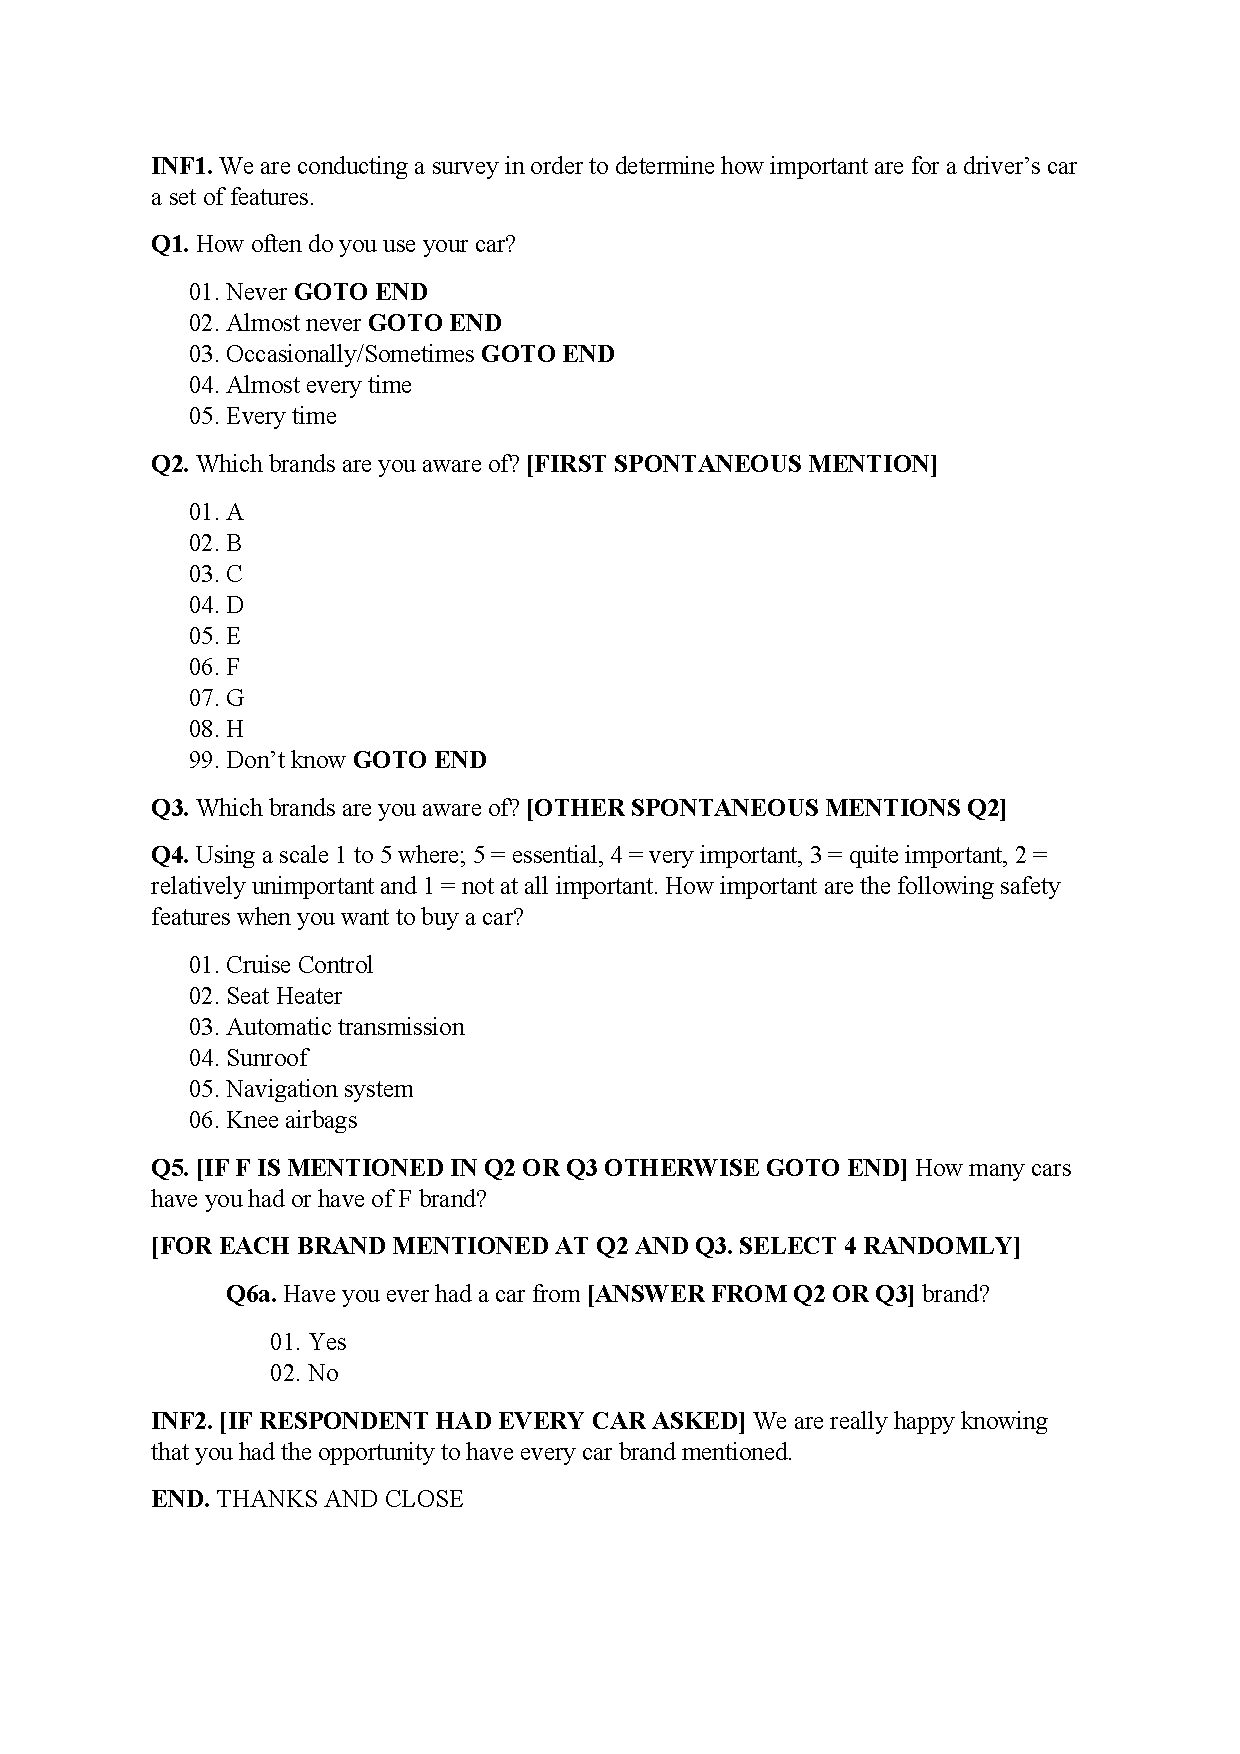
\includegraphics[max size={\textwidth}{\textheight}]{background/img/survey.pdf}
	\caption{Fully functional paper questionnaire instance}
	\label{fig:background:survey}
	\end{figure}

	

\section{Extensible Mark-up Language (XML)}\label{sec:background:xml}
		The web browsers use \gls{html} to build the presentation of information. They interpret each \gls{html} tag in order to display words, images or videos. However, this language is neither able to capture the description of contents, i.e. semantics, nor permits extending its mark-up with tags that are application-specific. In order to address these limitations, \gls{w3c} developed \gls{xml}. This meta-language, not only permits representing semi-structured data \cite{web:w3cxml} but also serves as a medium of communication that is widely used across Internet applications.

	\gls{xml} files are composed of elements, attributes and relationships \cite{book:varde2010}. Listings \ref{code:background:xmlCase} shows an \gls{xml} document example that describes a small questionnaire with two sections and their respective routing. Specifically, an \emph{element} is used to represent an entity which is enclosed through a start and end tag (e.g. survey, section, intro, single, multiple, routing and variable). An element may contain character data, other elements or a mixture of both within. Also, this may have \emph{attributes} whose presence is limited to the start-tag exclusively (e.g. id or ref).

	\lstinputlisting[caption={XML example case},label={code:background:xmlCase}]{background/xmlCase.xml}

	The \emph{relationship} captures the nesting of elements and permit creating for simple to complex structures. For instance, the section element has 'section1' as id attribute and contains multiple, single and intro elements as children. Similarly, a more complex structure is the survey root element that contains section and routing elements within.

	\gls{xml} only requires for documents to be \emph{well-formed}, i.e a valid \gls{xml} document according to \gls{w3c} must have:
	\begin{itemize}
		\item a unique single root element in which every other element is contained within,
		\item properly nesting of all the elements,
		\item presence of start and end tag for every element,
		\item and value for attributes enclosed with quotes.
	\end{itemize}

	However, \gls{xml} by itself is merely a standard notation which does not restrict the elements and attributes permitted or the structures and content allowed. Therefore, in order to differentiate well-formed documents from those that a valid according to an \gls{xml} authoring language, it is needed to formally define a schema by using an \gls{xml} schema language.
\section{Schemas Languages}\label{sec:background:xmlSchemas}
		\gls{xml} schema languages are formal languages used to define schemas. A schema represents the definition of the \emph{syntax} and \emph{semantics} that is allowed for an \gls{xml} authoring language \cite{book:moller06}. The syntax consist of defining the vocabulary of the language as well as the different structures in which the elements and attributes are permitted. In contrast, the semantics determines whether or not the syntax expressed in an \gls{xml} document is meaningful. 

	The use of a schema language to formalise an \gls{xml} authoring solution permits obtaining instance specifications that are non-ambiguous and benefits the software program that parses the instances since the number of errors can be reduced or eliminated. In order to check whether an \gls{xml} document conforms to a specific \gls{xml} language, a schema processor, which is an implementation program for an \gls{xml} schema language, takes two arguments: the \gls{xml} document or instance; and the schema (see Figure \ref{fig:background:validationProcess}). This processor, automatically decides the validity of a document and in addition, for those documents that are not valid, it provides a report document explaining the reasons of its failure.

	\begin{figure}[H]
	\centering
	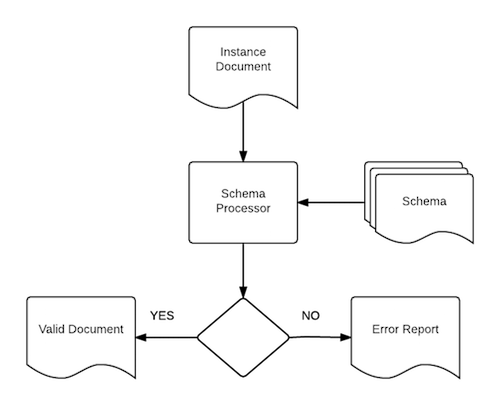
\includegraphics[width=0.75\textwidth]{background/img/validationProcess.png}
	\caption{XML validation process}
	\label{fig:background:validationProcess}
	\end{figure}

	During the process of validating \gls{xml} documents against an \gls{xml} language, four different levels of validation \cite{proc:stuhrenberg10} are checked in order to ensure the correctness of an \gls{xml} specification:
	\begin{enumerate}
		\item \emph{Structure}: This level validates the mark-up introduced as well as the order and occurrences of elements and attributes.
		\item \emph{Data-types}: At this stage it is determined whether the content defined for elements and attributes conforms to the data-types defined in the schema. 
		\item \emph{Integrity constraints}: This level verifies uniqueness of identifiers as well as checks that any reference points to existing keys. Usually, the keys and references to these, are values that are set for attributes.
		\item \emph{Business rules}: At this level, any additional data constraints \cite{proc:vandervlist06} that cannot be categorised in any of the above mentioned levels is checked. This level is very specific to the application domain in which the authoring \gls{xml} language was designed for. 
	\end{enumerate}

	The \gls{xml} schema languages are divided into two approaches: grammar-based and rule-based \cite{stuhrenberg13}. The grammar-based schema languages specify the mark-up, structure and data-types expected for \gls{xml} documents. For instance, they restrict the presence of attributes and elements, the type expected for values, the order in which elements or attributes may appear in the document or the minimum and maximum number of occurrences allowed. In contrast, the rule-based schema languages mainly ensure that the relationships among elements and attributes is consistent. However, they can also constraint \gls{xml} documents by incorporating business specific rules that make specifications meaningful for the application domain.

	Different schema languages exist today aimed to express constraints that are checked at any of the above mentioned validation levels. The three most popular grammar-based schema languages are \gls{dtd}, \gls{xsd} and \gls{relaxng}. Regarding the rule-based language formalisms, \gls{sch} is the only candidate representative. Table \ref{tab:background:schemasTable} summarises the validation levels that these schema languages support. Throughout the next following subsections, the schema languages most relevant to ensure the correctness of \gls{xml} specifications are explored.
	
	\begin{table}[h]
	\centering {\small{}}%
	\begin{tabular}{|c|c|c|c|c|}
	\hline 
	 & \textbf{\small{}DTD}{\small{} } & \textbf{\small{}XSD}{\small{} } & \textbf{\small{}RELAX NG}{\small{} } & \textbf{\small{}SCH}\tabularnewline
	\hline 
	\hline 
	\textbf{\small{}Structures}{\small{} } & {\small{}Basic } & {\small{}Yes } & {\small{}Yes } & {\small{}No}\tabularnewline
	\hline 
	\textbf{\small{}Data-types}{\small{} } & {\small{}Limited } & {\small{}44 built-in } & {\small{}Not directly } & {\small{}Not directly}\tabularnewline
	\hline 
	\multirow{3}{*}{\textbf{\small{}Integrity Constraints}{\small{} }} & ID & {\small{}unique} & \multirow{3}{*}{{\small{}Not directly }} & \multirow{3}{*}{{\small{}Yes}}\tabularnewline
	 & IDREF & key &  & \tabularnewline
	 &  & key-ref &  & \tabularnewline
	\hline 
	\textbf{\small{}Business rules}{\small{} } & {\small{}No } & {\small{}No } & {\small{}No } & {\small{}Yes}\tabularnewline
	\hline 
	\end{tabular}{\small{}\caption{Validation levels supported by the most popular XML schema languages}
	\label{tab:background:schemasTable} }
\end{table}

	\subsection{Document Type Definition (DTD)}\label{sec:background:dtd}

	\gls{dtd} is the built-in schema language since the first working draft of \gls{xml} \cite{web:w3cdtd}. There are many \gls{xml} authoring languages that are specified using \gls{dtd} such as \gls{xhtml} or \gls{triples}. The last mentioned, is known as the standard \gls{xml} language for describing questionnaires. \gls{dtd} has basic support to define syntax for documents since it is not possible to constraint the order and occurrences of elements when character data and elements are allowed within an element structure. Regarding the data-types, it is neither capable of constraining character data (e.g. id attribute for section starts with section followed by any number) nor allows frequent used types such as integer, date or \gls{uri}. In regard to the integrity constraints, it provides ID and IDREF for uniqueness and referential key respectively. However, any defined ID works for the entire document not being able to specify a more restricted scope (e.g. the question id cannot be duplicated across different sections). Moreover, compound keys, i.e. those that combine different attributes to form a key is not supported either. With regards to business rules, there is no mechanism that permits validating semantics over syntactically valid \gls{xml} instances. 

	\gls{dtd} was designed before the name-space mechanism was introduced. This feature, which permits reusing other schema specifications to create a new \gls{xml} language, is not provided and consequently it is not only hard to create modular schemas but also it is difficult to evolve them. Furthermore, a schema defined through \gls{dtd} does not use \gls{xml} notation so checking that a specification of an \gls{xml} language conforms to \gls{dtd} requires the use of non-standard \gls{xml} tools to verify its validity.

	\subsection{XML Schema Definition (XSD)}\label{sec:background:xsd}
	\gls{xsd} is the recommendation schema language for \gls{w3c} \cite{web:w3cxsd}. It was designed to be more expressive than \gls{dtd} and introduces name-spaces, data-types and an \gls{xml} syntax for restricting well-formed \gls{xml} files. As such, it permits importing structures of elements through the \gls{uri} mechanism, uses \gls{xml} syntax to express constraints, which eliminates the need to learn a new proprietary syntax and provides a richer built-in data-types system. Additionally, to strengthen the data-types set, it allows the definition of customised types through restriction (e.g. \gls{url} type is a subset of the string base type) and by extension (e.g. an element single question extends from question element by adding a set of open-closed response elements).

	This schema language unlike its counterparts, provides a better mechanism to express integrity constraints for \gls{xml} documents. \gls{xsd} overcomes the limitations of ID, IDREF that are present in \gls{dtd} by using a subset of XPath Query Language (see Section \ref{sec:background:xPath}) to define unique values for elements or attributes and to reference these through \emph{key} and \emph{key-ref} features respectively. For instance, Listings \ref{code:background:xsd} defines a key to ensure the uniqueness of a question (e.g. intro, single, multiple or open) in the context of a section from a survey through a \emph{selector} element. Moreover, to determine what attribute of a question element is used to check the uniqueness, the \emph{field} element is utilised. Similarly, in that example, the key-ref uses the selector to select a variable within a routing element in which the attribute ref is used to hold the reference to a unique question key. Note that key-ref also defines a refer attribute which points at a key element previously defined in the schema for an authoring language.

	\lstinputlisting[caption={Key and references in XSD},label={code:background:xsd}]{background/xsd_integrity.xml}

	The above mentioned integrity constraints could be used to verify that the document from Listings \ref{code:background:xmlCase} does not actually introduce duplicate keys for question ids neither specifies a reference to a non-existent question id within the routing. 

	\gls{xsd} is one of the most used schema language for defining \gls{xml} languages, mainly because supports enough expressiveness to define structure, data-types and integrity constrains for \gls{xml} documents. However, it is hard to learn due to the amount of features that provide and does not introduce any mechanism to express business rules. \footnote{The version 1.1. introduces assertions to express business rules through a subset of XPath expressions (attributes, children and descendants of an element) \cite{web:w3cxsdassertion}. However other existing relationships among \gls{xml} documents such as parent, ancestors or siblings are unable to express which restrict its expressiveness and usage.}

	\subsection{Regular Expression Language for XML New Generation (RELAX NG)}\label{sec:background:relaxNg}
	%http://www.iso.org/iso/home/store/catalogue_tc/catalogue_detail.htm?csnumber=52348
	\gls{relaxng} is a schema language developed within the \gls{oasis}. This language was built with the design principles of simplicity and expressiveness. As such, its syntax to express constraints for \gls{xml} documents is closer to plain English instructions \cite{book:vandervlist03}. \gls{relaxng} is part of the \gls{iso}/\gls{iec} 19757. Specifically, it is the candidate schema language for describing structure and content of \gls{xml} documents. 

	The data-types and integrity constraints are not directly supported by the language so it relies on external schema languages to address these tasks. Specifically, the data-types for elements and attributes are usually imported from \gls{xsd} whereas the integrity constraints are weakly supported by having a special compatibility data-type library that uses ID and IDREF from \gls{dtd}. Regarding the business rules, as this language is categorised as grammar-based, it does not directly offers features for specifying additional constraints.

	\subsection{Schematron (SCH)}\label{sec:background:sch}
	%http://www.iso.org/iso/home/store/catalogue_tc/catalogue_detail.htm?csnumber=55982
	\gls{sch} is a schema language designed by Rick Jelliffe \cite{web:doodds01}. This language differs from grammar-based \gls{xml} schema languages in that it is rules-based, i.e. defines assertions within a rule context that are evaluated over \gls{xml} instance documents. This language, likewise \gls{relaxng}, also takes part from the \gls{iso}/\gls{iec} 19757 and constitutes the standard reference to ensure that documents match the rules defined through a schema. In \gls{sch}, the constraints are specified via XPath query language (see Section \ref{sec:background:xPath}). The use of these expressive queries, permits defining any kind of tree relationships (e.g. child, parent, ancestor) that are inherited in \gls{xml} documents making this schema language unique in terms of expressing semantics.

	The core constructs of Schematron are patterns, rules and assertions. Listings \ref{code:background:schematron} describes an integrity constraint that check the uniqueness of section identifiers. The pattern element is used to group different rules. A rule requires a context attribute which constitutes the path used to evaluate one or more asserts (e.g. this rule is fired for every section within the survey element). An assert is specified through the test attribute and addressed to check a constraint within the context rule described. For instance, the assert example counts the preceding section's identifiers that are equals to the identifier set through the place holder \$id (e.g. let element) in order to determine whether is zero or not. A false result for the assert, displays the customised message within that element.  
	\lstinputlisting[caption={Integrity constraint expressed in SCH},label={code:background:schematron}]{background/sch_integrity.xml}

	The validation of \gls{xml} documents against a \gls{sch} schema can be carried out either by using an \gls{xslt} \cite{web:w3cxslt} processor or by using an XPath implementation. The \gls{xslt} approach, represented in Figure \ref{fig:background:sch_xslt_processor} requires performing two steps:

	\begin{figure}[H]
	\centering
	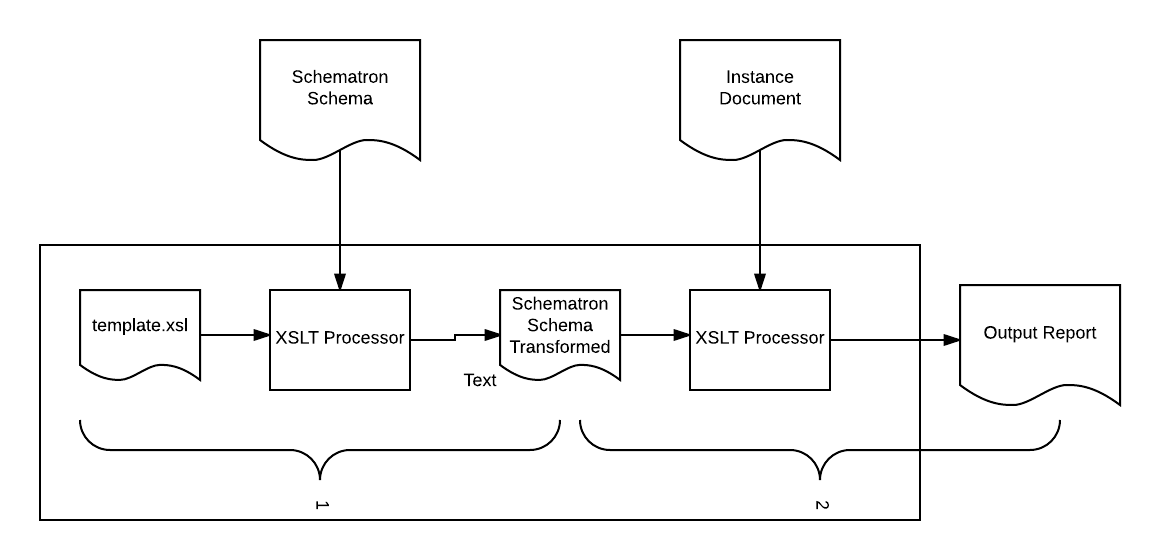
\includegraphics[width=0.90\textwidth]{background/img/sch_xslt_processor.png}
	\caption{Schematron XSLT validation process}
	\label{fig:background:sch_xslt_processor}
	\end{figure}

	\begin{itemize}
		\item First, an \gls{xslt} processor gets a \gls{sch} schema together with a pre-defined \gls{sch} template, provided by Academia Sinica Computing Centre \footnote{\url{https://www.ascc.sinica.edu.tw/en/about/overview.html}}, in order to produce a transformed \gls{sch} schema understandable by the \gls{xslt} processor.
		\item Second, the transformed schema, together with the \gls{xml} document is passed to the \gls{xslt} processor to finally produce the output report based on the rules and assertions in the original \gls{sch} schema defined.
	\end{itemize}

	The XPath implementation, unlike its counterpart, is faster for validating \gls{xml} documents since the transformation step is not needed. However, it has less functionality due to \gls{xslt}-specific functions such as document() or key() which are not supported. For instance, \emph{document} function permits validating rules among \gls{xml} documents.

	The high expressiveness of \gls{sch} not only makes this schema language the best for representing any integrity constraint \cite{art:murata05} but also extends its capacity to define any sort of business rule. Regarding the structure, although it is able to describe many instances of grammars \cite{web:jellife07}, this constraining level is best addressed through grammar-based languages. In regard to the data-types, \gls{sch} does not directly provide any built-in type. However, these may be simulated using the XPath functions.
\section{XPath Query Language}\label{sec:background:xPath}
		XPath is a query language that uses path expressions to navigate through \gls{xml} documents. It is the recommended query language for \gls{xml} documents by \gls{w3c}. \gls{sch} was the first schema language that used XPath for expressing rules and after \gls{xsd} borrowed this idea to specify its integrity constraints. The syntax used in this query language is based on a location path, i.e. a similar concept used in file systems, which consist of a sequence of location steps:
	\begin{itemize}
		\item axis to direct the navigation with the relationships parent, children, siblings, ancestors or descendants \cite{web:w3caxes} since this language treats the \gls{xml} files as trees of nodes,
		\item node test that permits filtering the path to a specific node or element and
		\item predicates which allow selecting only those nodes with specific properties or attributes.
	\end{itemize}

	To better understand how this syntax works, we show some examples using the \gls{xml} document from Listings \ref{code:background:xmlCase}. For instance, in order to select the section 1 element and children, we could express /survey/section[@id='section1'] with the node test /survey/section and the predicate specified in brackets, but we could be more specific about retrieving only the ids of the questions /survey/section[@id='section1']/child::node()/@id. Note, that the first example obviates the axis, i.e. the expression has been defined using the \emph{abbreviated mode}, which is more compact. In contrast, the second one explicitly uses the axis to guide the location deeper in the sub tree /survey/section and it is known as \emph{full syntax mode}.
\section{Conclusion}
		Our \gls{cawi} system solution for survey life-cycle adopts \gls{rest} constraints to adhere to scalability, simplicity and reliability architectural properties expected for \gls{cawi} systems. Particularly, the \gls{rest} \gls{api}, which conforms to the \gls{http} protocol, has been implemented with the standard reference library for Java. This multi-layered solution is highly portable and uses a \gls{nosql} database solution which permits a more flexible persistence solution when compared to the traditional relational databases.

	The client side, based on the \gls{spa} not only improves the responsiveness of a distributed system but also helps to produce richer interactive interfaces. This paradigm when compared to the multi-page approach that \gls{cawi} systems such as Blaise or SurveyMokey adopt, is more attractive. Particularly, with the choice of AngularJS as the framework for building pages, we have gained a simplified cross browser testing of functionalities, reduced the server burden by transferring interface logics to the client and promoted a parallel development of design and collection interfaces.


\chapter{Literature}\label{ch:literature}
		This Chapter presents \gls{cawiml} as an alternative authoring language to specify questionnaires only using standard \gls{xml} schema languages. Particularly, it uses a state-transition paradigm for question's sequence and is intended to facilitate the questionnaire routing logic more adequately than the popular hierarchical model. \gls{rpn}, is the expression formalism utilised for describing routing and personalisation constructs indistinctly.

	The rest of this Chapter is structured as follows: Section \ref{sec:cawiLanguage:stateTransition} introduces the state-transition routing structure. Section \ref{sec:cawiLanguage:rpn} explains the postfix notation mode as the formalism for questionnaire expressions, followed by Section \ref{sec:cawiLanguage:xmlLanguage} that explains our \gls{xml} authoring solution. Finally, \gls{xml} details for content, routing and personalisation constructs expressed in \gls{cawiml} are presented in Section \ref{sec:cawiLanguage:cawiml}.
	 
\section{The XML Languages}\label{sec:literature:xmlLanguages}
		The most relevant \gls{xml} languages addressed to cover questionnaire constructs are \gls{triples}, \gls{sss}, \gls{qdl} and \gls{ddi}. The following sections provide a brief description of each authoring solution before conducting a comparative analysis.

	\subsection{Survey Interchange Standard (Triple-S)}
			%Triple-S is aimed to describe the key elements of surveys \cite{book:triplesxml} in order to make easier the transfer of data and meta data between survey or analysis software packages. Wright describes an use case tool which accepts data in triple-S format to take business decisions \cite{proc:wright07}.

	%This language was first published in 1994 and since then three major versions have been released. The latest one (2.0) defines two files: the \emph{definition File} which contains general information and survey variables (i.e. the meta data) and the \emph{Data File} storing data for a meta data instance. This version supports \gls{csv} format for exporting the survey data as well as the ability to specify hierarchies. The hierarchy feature results useful for questionnaires where exist a relationship parent-children (e.g. a household questionnaire contains questions at the household level and a set of questions to be repeated for each member of the household). This relationship is defined through a specification control file.

	\gls{triples} is aimed to represent the content aspects of surveys \cite{book:triplesxml} in order to make it easier to transfer data and meta data among \gls{cai} systems or any analysis software package. This language is considered the standard for representing social surveys and at least fifty registered implementers may be found on its website \cite{web:triples}. Although its focus has been to provide a comprehensive coverage of survey functionality, we have found one case study where \gls{triples} has been adapted to describe a business decision making tool \cite{proc:wright07}.
	\subsection{Questionnaire Definition Language (QDL)}
			%\gls{qdl} is an \gls{xml} language developed as part of the \gls{tadeq} project. \gls{tadeq}'s aim is building a software tool for translating questionnaire specifications from different \gls{cai} systems in a human-readable format \cite{proc:bethlehem00}. This tool is able to generate two types of documentation: \emph{textual}, providing detailed information on all questionnaire constructs and \emph{graphical}, assisting in the understanding of the routing structure. The tool attempts to be helpful for different target people: \emph{questionnaire developers} who want to document their work, \emph{survey managers} who have to give formal approval to execute the survey and \emph{interviewers} who want the documentation to help them when they are collecting responses.

	%\gls{tadeq} accepts \gls{xml} instances according to \gls{qdl} which means every \gls{cai} survey system has to create its own converter from its authoring questionnaire language to \gls{qdl} (e.g. Blaise system has its own converter). \gls{qdl} is focused on design and collection stages of surveys and is able to describe filter and skip constructs indistinctly.

	\gls{qdl} is a language built for \gls{tadeq} project whose aim is at building a software tool that represents questionnaire specifications in a human-readable format \cite{proc:bethlehem00}. This tool can operate in either textual or graphical mode. It is suited to designers who want detailed information of the constructs and interviewers who need documentation to help them when they are conducting interviews. Although this project has some implementers like Blaise that has its own converter, this project has been abandoned and there is no longer support for this language.





	\subsection{Data Documentation Initiative (DDI)}
			\gls{ddi} emerged in 1995 as an international project to create standardised meta data to document social science datasets \cite{art:rasmussen07}. It emerged to solve the problems of documenting datasets and introduces \gls{xml} as the exchangeable data format to be both, machine-readable and human-understandable. It has an important value for analysis and archiving since permits describing data at two levels: \emph{variable} level, which consist of describing the different variables involved on the research; and \emph{study level}, since it allow describing the population that links to the stored information. 

	In its third version was introduced the description of social surveys. Since then, the \gls{abs} has been experimenting with this exchangeable format for their design tool for questionnaires. Similarly, \gls{insee}, that uses Blaise \gls{cai} system for collecting data has shown interest on using \gls{ddi} as a standard to communicate different disciplines in the data collection field. For that purpose, a \gls{pof} was created by de Bolster to convert from Blaise language specifications to \gls{ddi} 3.1. From that experiment, it was concluded that neither \gls{ddi} instances are human readable nor compatibility between different versions is considered. For instance, when valid \gls{ddi} instances for questionnaires were verified against the schemas of the newer version at least 365 errors occurred \cite{proc:bolster13}.
	\subsection{Simple Survey System (SSS)}
			%-The response data is stored in XML files
	%-The survey engine runs C++.
	%-Rules are defined in \gls{xsd}.
	%-Number and type of arguments cannot be validated when the questionnaire specification file is read. Argument validation must wait until the function is actually invoked.
	%-Expressions are evaluated recursively from inside out.
	%-Functional approach leds to expressive structurefor representing calculations and expressions

	%\gls{sss}, known as a \gls{capi} system solution developed for \gls{rti} which has its own \gls{xml} specification language to address the questionnaire constructs \cite{art:bethke08}.
	%This language has a different approach to define its logical and arithmetical expressions based on a functional programming style which makes the authoring language more robust and less prone errors.
	\gls{sss} is a \gls{capi} system solution developed for \gls{rti} which has its own \gls{xml} language to address content, routing and personalisation features of surveys \cite{art:bethke08}. This language unlike \gls{triples}, \gls{qdl} or \gls{ddi} has a robust schema to represent the logical and arithmetical expressions based on functional programming style. 


\section{Comparative Analysis of XML Languages}\label{sec:literature:comparativeAnalysis}
		In this section we detail a comparative analysis of the \gls{xml} authoring languages used to define questionnaire specifications. For that purpose, we explore the coverage of routing and personalisation constructs in Section \ref{sec:literature:routing} and \ref{sec:literature:personalisation} respectively. The relevant flow paradigms used to capture the routing sequence for questionnaires is explained in Section \ref{sec:literature:flowParadigm}. The constraining level coverage of the schema languages used to define these \gls{xml} languages is addressed in Section \ref{sec:literature:schemaLanguages}. Section \ref{sec:literature:expressionNotation} studies the three notation to describe logical and arithmetical expressions through an example from a real questionnaire and finally the survey life-cycle stages in which every \gls{xml} language is focused on is detailed in Section \ref{sec:literature:surveyStages}. Table \ref{tab:literature:comparison} summarises the above mentioned aspects that will be treated on the next sections.

	\begin{sidewaystable}
	\begin{center}
	\begin{tabular}{|c|c|c|c|c|c|}
	\hline 
	\textbf{\textcolor{blue}{\emph{Category}}} & \textbf{\textcolor{blue}{\emph{Feature}}} & \textbf{\textcolor{blue}{\emph{Triple-S}}} & \textbf{\textcolor{blue}{\emph{SSS}}} & \textbf{\textcolor{blue}{\emph{QDL}}} & \textbf{\textcolor{blue}{\emph{DDI}}}\tabularnewline
	\hline 
	\hline 
	\multirow{5}{*}{\textbf{\textcolor{blue}{\emph{Routing}}}} & \textbf{Skip} & No & No & Yes & No\tabularnewline
	\cline{2-6} 
	 & \textbf{Filter} & Partial & Yes & Yes & Yes\tabularnewline
	\cline{2-6} 
	 & \textbf{Loop} & No & Yes & Partial & Yes\tabularnewline
	\cline{2-6} 
	 & \textbf{Check} & No & No & Yes & No\tabularnewline
	\cline{2-6} 
	 & \textbf{Computation} & No & Yes & Yes & Yes\tabularnewline
	\hline 
	\multirow{4}{*}{\textbf{\textcolor{blue}{Personalisation}}} & \textbf{Piping - text-fill} & No & Yes & No & Yes\tabularnewline
	\cline{2-6} 
	 & \textbf{Piping - carry-forward} & No & No & No & No\tabularnewline
	\cline{2-6} 
	 & \textbf{Randomising} & No & No & No & Partial\tabularnewline
	\cline{2-6} 
	 & \textbf{Rotating} & No & No & No & Partial\tabularnewline
	\hline 
	\multirow{4}{*}{\textbf{\textcolor{blue}{\emph{Other}}}} & \textbf{Flow Paradigm} & N/A & Hierarchical & Hierarchical & Hierarchical\tabularnewline
	\cline{2-6} 
	 & \textbf{XML Schema Language} & DTD & XSD 1.0 & DTD & XSD 1.0\tabularnewline
	\cline{2-6} 
	 & \textbf{Expressions Notation} & N/A & PreFix & Infix & Infix\tabularnewline
	\cline{2-6} 
	 & \textbf{Survey Stage} & Analysis/Reporting & Design/Collection & Design & Analysis/Reporting\tabularnewline
	\hline 
	\end{tabular}
	\caption{Comparison of XML languages for electronic questionnaires}
	\label{tab:literature:comparison}
	\end{center}
	\end{sidewaystable}
	\subsection{Routing Constructs}\label{sec:literature:routing}
			The filter construct is well represented by \gls{sss}, \gls{qdl} and \gls{ddi} whereas it is partially described by \gls{triples} since this language is only able to represent simple logic involving only one variable. 

	In contrast, the skip logic is only defined by \gls{qdl} which considers the fact that for questionnaire designers it is difficult to express conditional statements \cite{proc:katz97}. However, as far as we know, the tool that implements this language does not offer support since it is difficult to implement conditions without having restrictions over the type of jumps allowed \cite{art:bethlehem04}. The other languages do not cover this construct either because the skips can be reversed and use filters instead \cite{art:bethke08} or since surveys designed without unstructured patterns are easy to modify, share and understand \cite{web:spencer12}. %NOT CLEAR SKIP REVERSED AND USE FILTERS INSTEAD

	The loop construct is well represented in \gls{sss} and \gls{ddi}. Despite the fact that \gls{ddi} offers three types of loops (RepeatUntil, RepeatWhile and range loop) \cite{man:thomas09}, we consider that \gls{sss} is more flexible than \gls{ddi} to define expressions since it embodies a simple functional programming style through the use of \gls{xml} tags. In spite of \gls{qdl}, it only offers support for range loop but does not consider iterations over lists (see the instruction after Q5 in Figure \ref{fig:background:survey}). Regarding \gls{triples}, it does not directly define any mechanism to iterate, although offers an interesting feature to relate data collected from hierarchical surveys (e.g. survey responses for a household survey followed by responses of the property members defined in another survey) \cite{proc:wright07}.

	The check construct is only featured in QDL and this is likely to be motivated by the need to describe multi-item constraints to check consistencies among answers to related questions \cite{proc:katz97} or alternatively because this XML language is strongly related to Blaise system \cite{proc:bethlehem00}. Regarding the computation feature, other than Triple-S, all others languages support its representation.

	\subsection{Personalisation Constructs}\label{sec:literature:personalisation}
			Although \gls{sss} and \gls{ddi} offer mechanisms to describe \emph{text-fill} aspects, the other piping feature, i.e. the \emph{carry-forward} has not been considered. This construct, which permits describing operations to retrieve selected on unselected responses from previous questions as part of the responses for other questions (see Q3 from Figure \ref{fig:background:survey}), may help to better adapt surveys for each respondent. Accordingly, we consider that a specification language cannot leave out this construct. For instance, the popular SurveyMonkey \gls{cawi} system, we have observed that it implements this personalisation feature as part of its interface functionalities.

	Regarding the randomising and rotating features, these constructs are only partially covered by \gls{ddi} permitting to change the order for content constructs such as single and/or multiple question responses. However, more sophisticated patterns like selecting a specific number of responses after randomising/rotating or reordering only a subset of responses is not taken into account. For instance, the instruction above Q6a from Figure \ref{fig:background:survey} not only specifies to randomise the elements selected but also requires to iterate a maximum of four times.

	\subsection{Routing Flow Paradigms}\label{sec:literature:flowParadigm}
			The questionnaire's flow captures the sequence for the question constructs defined in a questionnaire. The designers or social researchers commonly use skip patterns that can be interchanged with filters to express the logical order of elements in a questionnaire. We have explored the directed graphs, Petri Nets and the hierarchical paradigms in order to %find out whether these approaches describe questionnaires in a structured manner but permitting designers to express logics through skip patterns.
	establish the suitability for representing sequence logic.

	The \emph{directed graph}, was explored in the past by Fagan et al. in order to analyse the use of skip constructs on surveys. These graphs based on \emph{nodes} and \emph{arcs} are able to represent question and response choices respectively. %Moreover, the source and sink properties of the graph correspond to the first and last question of a questionnaire. 
	When additional information such as the conditions that determine the ordering of questions are added to these graphs, they become flowcharts which result in tools to document and understand questionnaire's flow \cite{art:jabine85}. The directed graphs, permit validating the correctness of data gathered from surveys by detecting whether or not a question response is missed or is not applicable. These verifications are conducted applying different graph properties \cite{tech:fagan88}. Although the properties from graphs can be used to model the flow of questionnaires, as far as we know, this paradigm has not been used to formally define questionnaire specifications in \gls{xml}.

	In more recent work, Petri Nets have been applied to visualise and analyse complex questionnaires \cite{proc:rolke10}. Figure \ref{fig:literature:pretiNet} illustrates the Petri Net representation on part of the questionnaire from Figure \ref{fig:background:survey} in relation to question Q1 and the skip construct that permit navigating either to Q2 or END. %A more recent study case carried out by Rolke is concentrated on the visualisation and analysis of a complex questionnaire using Preti Nets. Figure \ref{fig:literature:pretiNet} contains a small portion of this net that represents part of the paper questionnaire from Figure \ref{fig:background:survey}. Specifically, it is depicted the question Q1 and the skip construct that permit navigating either to Q2 or END. 
	Here a \emph{place} (e.g. Q1, Q2 and END) captures the static information from a question whereas a transition (e.g. 01, 02, 03, 04, 05) represents a response choice. Additionally exist \emph{arcs} to connect places to transitions (e.g. arrow connecting Q1 to 01) and vice versa (e.g. 01, 02 and 03 to END). A Petri Net permits validating the \emph{reachability} of places, i.e. checking whether or not a set of responses given for questions correspond to a valid state of the net. However, this modelling approach is only limited to finite domain, i.e. it is only applicable for single and multiple questions, but becomes hard to manage open questions since an arc connecting places to/from transitions has to be specified for any possible value expected.

	\begin{figure}[h]
	\centering
	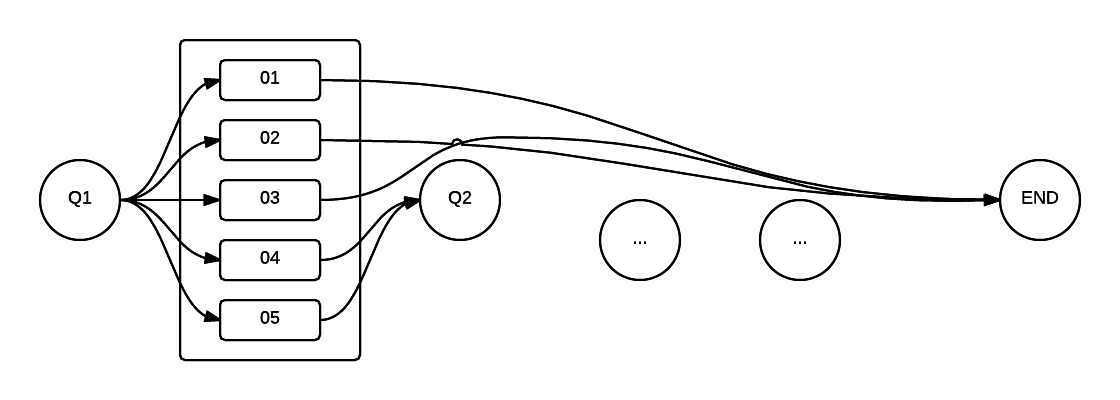
\includegraphics[max size={\textwidth}{\textheight}]{literature/img/pretiNet.png}
	\caption{Petri Net instance}
	\label{fig:literature:pretiNet}
	\end{figure}

	\gls{sss}, \gls{ddi} and \gls{qdl} adopt a hierarchical modelling approach where the use of skip pattern is avoided in favour of structured constructs (if-then-else, loops and sequences) as advocated by Dijkstra \cite{art:dijkstra68}. As such, the routing structure of surveys can be seen as trees permitting not only the identification of the path followed but also determining all the circumstances under which a question may be triggered \cite{web:spencer12}. Algorithm \ref{alg:hierarchical} describes in pseudo-code the routing of the questionnaire from Figure \ref{fig:background:survey} according to the hierarchical modelling. Note how the nesting of constructs is used to avoid skips. However, this nesting is not naturally well suited to reusability.%WEIRD does not naturally well suited ...

	\begin{algorithm}
	INF1\;
	Q1\;
	\If{NOT(Q1 IS\_SEL '01' OR Q1 IS\_SEL '02' OR Q1 IS\_SEL '03')}{
		Q2\;
		\If{NOT(Q2 IS\_SEL '99')}{
			Q3\;
			\If{NOT(Q3 IS\_SEL '99')}{
				Q4\;
				\If{Q2 IS\_SEL '06'}{
					Q5\;
					\For{each Q2 SEL}{
						Q6a\;
					}
					\If{HAD\_CAR \textgreater 1}{
						INF2\;
					}
				}
			}
		}
	}
	END\;
	\caption{Hierarchical modelling example}
	\label{alg:hierarchical}
	\end{algorithm}

	The benefits of eliminating skip patterns are universally acknowledged by high-level programme languages architects, however designers or social researchers still specify questionnaires through documents using skips to navigate from one question to another \cite{proc:katz97}, not only because they do not have programming skills but also because the final client interested in the survey, demands plain English instructions. As the hierarchical approach replaces the use of skip constructs, there is an evident \emph{gap} between what the social researchers design versus the \emph{code} that a \gls{cawi} system uses to execute a survey. Costigan states that having two sources of specification, i.e. the code and the document requires duplication of effort and it is prone to error \cite{proc:costigan03}. To unify these two sources, Spencer proposes that researchers should be trained to use structured patterns \cite{web:spencer12}, i.e. avoid the use of skip constructs. However, in practice, motivating social researchers to adopt this practice remains a problem \cite{proc:costigan03}. %few social researchers would be interesting in eliminating skip patterns from questionnaire specifications \cite{proc:costigan03}.

	The ability to introduce changes to questionnaires is another factor to consider since clients often demand the modification of survey logics when the data collection is already taking place. This involves having a modelling approach that addresses the \emph{adaptability} appropriately. It is evident from the above hierarchical representation that strong coupling between the inner and outer filters increases with increasing skip constructs. %It is evident by examining the above example introduced, that exist coupling between the inner and outer filters which increases when newer skip constructs are added. 
	As dependencies among constructs are like to impact negatively to changes to questionnaire's flow, there is a need to explore a less intrusive model.
	

	\subsection{Schema Languages}\label{sec:literature:schemaLanguages}
			The different \gls{xml} languages reviewed are formally defined through an \gls{xml} schema. Specifically, they use grammar-based schemas to define the vocabulary, structure and data-types expected for instances defining a questionnaire. Throughout this section, the \gls{xml} example from Listings \ref{code:background:xmlCase} will be used to discuss features supported by \gls{dtd} and \gls{xsd}.

	\gls{qdl} and \gls{triples} are defined using DTD (see Section \ref{sec:background:dtd}). This schema formalism has two weaknesses: inability to express complex structures for elements; and limited number of data-types whereby common types such as number or date are not supported.%\gls{triples} and \gls{qdl} are defined using \gls{dtd} (see Section \ref{sec:background:dtd}). This schema formalism is known for its limitations to express complex structures for elements as well as for its very limited data-types set where commonly types such as numbers or date are not supported. 
	With regards to the integrity constraints, the ID and IDREF mechanisms, offered for describing uniqueness of elements and references to valid identifiers respectively, are not robust enough for expressing semantic constraints over \gls{xml} documents. Specifically, the lexical space of an identifier is global to the entire document (e.g. the question id cannot be duplicated across different sections) and as Fan and Simeon state, this is a very strong restriction for a schema language \cite{art:fan03}. Moreover, the IDREF is not able to point to a specific key identifier (e.g. it cannot be described such that the ref attribute for a routing element links to the identifier attribute of a section). Regarding the business rules level, there is no such feature to constraint the additional semantics for \gls{xml} documents.

	\gls{sss} and \gls{ddi} use a more expressive schema language that was built to address the limitations of \gls{dtd}. Most structures are supported in \gls{xsd}. Its very rich set of data-types goes farther than simply supporting only common type such as string, boolean, decimal, integer or date to permitting the definition of any customised type through regular expressions. Regarding the integrity constraints, although a more expressive mechanism using key and key-ref through XPath expressions is provided (see Section \ref{sec:background:xsd}), not every possible relationship existing in \gls{xml} documents can be defined \cite{web:w3cxsdassertion}. Specifically, in \gls{xsd} the XPath expression for a \emph{xs:selector} can only use children and descendants of the element in which it is defined. In addition, the \emph{xs:field} restricts the XPath expressions to only select attributes \cite{proc:vandervlist06}. For instance, it is not possible to constraint the variables Q0, Q1 or Q2 such that they can point to questions defined in 'section1'. With respect to the business rules, only \gls{xsd} 1.1, which is not used neither in \gls{sss} nor \gls{ddi}, supports assertions to express additional semantics for \gls{xml} documents. However, the XPath expressions are equally limited to attributes, children and descendants of the node where the assertion has to be checked.

	The grammar-based schema languages are adequate to specify mark-up and syntax for \gls{xml} documents, however they are insufficient to express integrity constraints or business rules. Accordingly to address these issues it is best to use a rule-based schema languages such as \gls{sch} which has no restrictions on XPath expression definitions. %The grammar-based schema languages are adequate to specify mark-up and syntax for \gls{xml} documents, however they are insufficient to express any kind of integrity constraint or business rules. To better address these two other constraining levels, it is best the usage of rule-based schema languages such as \gls{sch} since there are no restrictions to define XPath expressions. 
	Therefore, if the well defined patterns from grammar-based languages are combined with the expressiveness of rule-based schemas \cite{proc:vandervlist06} \cite{web:costello15} \cite{art:lee00}, it is possible to create an \gls{xml} authoring solution that is better suited to handle the different validation stages, i.e. a language that ensures the correctness of questionnaire specifications without the necessity of relying on programming languages to validate complex semantic constraints.


	\subsection{Expressions Notation}\label{sec:literature:expressionNotation}
			The routing constructs contain logical and arithmetical expressions applicable for filters, loops, checks and computations. Typically these expressions are defined using infix style. For instance, questionnaire languages such as \gls{qdl} and \gls{ddi} use this mode. Consider the following infix notation example, that follows the normalised convention proposed by Hughes \cite{proc:Hughes07} as an attempt for describing expressions in paper questionnaires:

	\textbf{ASK IF:} [QB = 'Male' AND (QA = 'Scotland' OR QA = 'Wales') AND (Q5 = 'Less' OR Q5 = '1-3')], \emph{[Ask males in Scotland and Wales who eat less than or equal to 3 portions of vegetables per week]} \footnote{Expression extracted from survey 08 of the Appendix \ref{sec:appendix:questionnaires}}

	Firstly, the filter construct (ASK IF) as described, secondly an algebraic expression is defined and finally a plain English instruction is provided in order to be more readable. Although this notation constitutes the natural way of thinking, the inclusion of brackets becomes a necessity in order to override the operators precedence.

	Unlike the infix notation, with prefix and postfix notations where the operators are written before and after their operands respectively. Here the operators are no longer ambiguous with respect to the operands and consequently the parentheses may be obviated. Accordingly our example in prefix notation can be stated as follows:

	\emph{AND AND = QB 'Male' OR = QA 'Scotland' = QA 'Wales' OR = Q5 'Less' = Q5 '1-3'}

	And the postfix representation is:

	\emph{QB 'Male' = QA 'Scotland' = QA 'Wales' = OR AND Q5 'Less' = Q5 '1-3' = OR AND}.

	\gls{sss} uses the prefix mode through a functional programming style inspired by Lisp Language which is a more desirable approach to choose. However, when prefix mode is compared with postfix notation, it is less efficient because the order that the operators have to be evaluated does not strictly follow the left-to-right order, i.e. the operators placed on the left, must wait until the intermediate operations on the right part are solved (e.g. the first and second AND operators). This involves moving backward and forward through the structural representation of the expression, increasing the number of operations. With respect to postfix mode, there is no need for operands to wait (e.g. the last two operators OR, AND) have the intermediate results solved before being evaluated and consequently it is computationally most effective.

	\subsection{Survey Stages}\label{sec:literature:surveyStages}
			Survey research is a process that goes beyond asking a set of questions \cite{booklet:ibm12}. As part of this research process, the survey may be divided into five stages (see Figure \ref{fig:literature:5stages}). These stages are \emph{design}, that involves the formulation of questions needed for the achievement of the aim and objectives. The \emph{collection}, where an instrument such as a questionnaire is used in order to obtain responses to the formulated questions. The \emph{management}, aimed at monitoring the results gathered and helpful to determine the presence of any problematic question. The \emph{analysis}, that consist of conducting different statistics to study the data collected and finally the \emph{reporting} where different artefacts such as documents, tables, graphs or charts are used to present the data gathered in order to help decision making. This stage may serve also as a mechanism to export data and meta data into different formats such as \gls{csv} that may be utilised by more sophisticated software vendors such as SPSS to conduct advanced analytics.

	\begin{figure}[h]
	\centering
	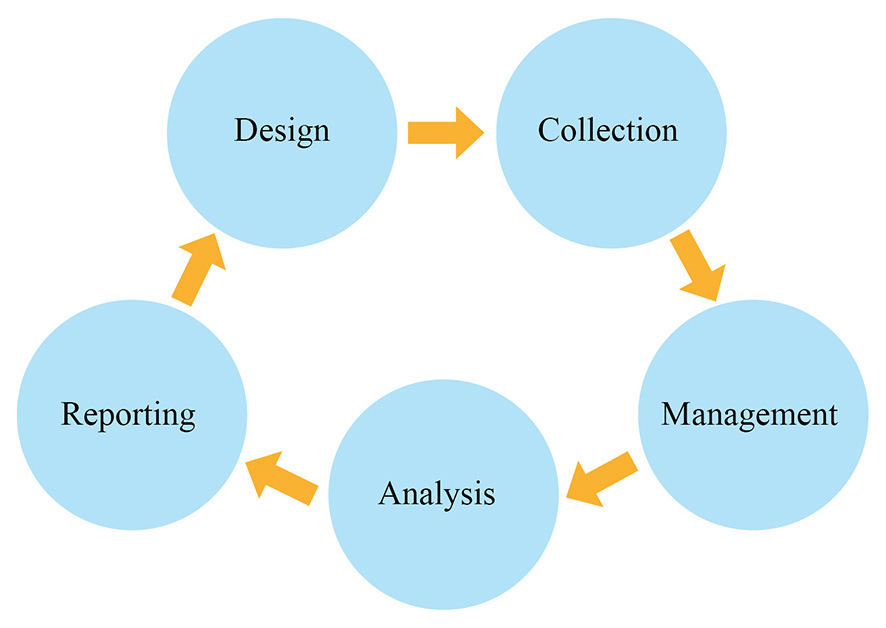
\includegraphics[width=0.75\textwidth]{literature/img/5stage.jpg}
	\caption{The 5 stages of survey research}
	\label{fig:literature:5stages}
	\end{figure}

	The authoring languages studied are focused on one or more stages of the survey research cycle. For instance, \gls{triples} and \gls{ddi} pay special attention to analysis and reporting stages since they provide structures that permit exporting the data collected for a questionnaire as well as its associated meta data. 
	In contrast, \gls{qdl} is best suited to address the design stage since it is built as part of a project to develop a tool for documenting questionnaire specifications \cite{man:bethlehem02}. 

	Whilst \gls{sss}, although was built to facilitate the creation of intuitive interfaces for supporting the design stage, it is more adequate to drive the collection stage given its formalism to describe expressions which offers more advantages than its counterparts and permits reducing the number of validations that have to be carried out before executing a questionnaire.
		
\section{CAWI Systems}\label{sec:literature:cawiSystems}
		\gls{cawi} systems are based on a \gls{cs} architecture style that uses \gls{http} to communicate between client and server. Several refinements for this basic architecture have been made over the years such as the \emph{distributed objects} style (e.g. \gls{corba}), which uses the object-oriented paradigm, for client server communication by encapsulating data and behaviour together \cite{proc:overdick07}. This approach is not appropriate for distributed environments since it asserts too much responsibility on the client which has to manage the life-cycle of objects, i.e. operations such as create, copy, move or destroy, and the server that has to rely on these operations performed.

	A more modern architecture style is \gls{soa} that defines services to address the different functionalities of a system. In this approach, there are two agents involved: the \emph{provider}, which implements a defined business function that operates independently of any other service provider; and the \emph{consumer} which uses the service \cite{tech:mackenzie06}. The interactions among the agents are performed through different communication protocols such as \gls{soap} and using standard exchangeable formats like \gls{xml}.

	As Pexel company demands the design and development of a new \gls{cawi} solution that can offer potential advantages over competitors, we consider that it is important to evaluate different architectural properties for the existing \gls{cawi} systems in order to determine how they address the simplicity, portability, reliability and scalability. Similarly, as the software system is network-based, it is crucial to review different test strategies for performance since these may help to estimate response times that in term, impact usability.

	The rest of this section is structured as follow: Section \ref{sec:literature:architectures} reviews the architectural style of different \gls{cawi} systems and Section \ref{sec:literature:performanceTesting} explores different testing methods and parameters used to simulate scenarios for performance testing of \gls{cawi} systems.





	\subsection{CAWI System Architectures}\label{sec:literature:architectures}
			This Section explores Blaise and SurveyMonkey architectures in order to determine the architectural properties being adopted by \gls{cawi} systems. However, other software solutions such as \gls{cases}, have not been explored due to the absence of publicly available documentation.

	\subsubsection{Blaise}\label{sec:literature:blaise}
	%This style permits developers to focus on a specific role, i.e. they can implement and maintain isolated services, multiple applications can reuse services code and the testability is improved.
	The architecture style of Blaise is \gls{wcf}, which is an implementation of \gls{soa}. In this style, the interactions among components is carried out by sending data through asynchronous messages that can be either \gls{xml} formatted or using complex streams of binary data. The \gls{cawi} solution offered by Blaise, separates the functionalities into different roles (see Figure \ref{fig:literature:soaBlaise}) \cite{proc:segel15}. The most important server roles are: \emph{survey manager}, that holds the creation and publishing of surveys; \emph{data entry server}, used to validate input and routing logic; \emph{data server}, that performs read/write operations into the databases; \emph{session server}, that stores and controls the active interviews; and \emph{web server} used to host and serve web pages to the end users. %This role uses the \gls{mvc} design pattern that offers benefits such as loose coupling due to the separation of concerns, it helps to manage the application when becomes more complex or promotes parallel development (e.g. one developer can focus on the model, a second can concentrate on the controller and a third one on the view). Nevertheless, we consider that this component can be moved to the client-side since browsers nowadays have mature JavaScript frameworks able to apply this design pattern. Hence, this suggestion may produce a much better user experience and help to reduce network latency since only data in \gls{json} or \gls{xml} format is sent.

	\begin{figure}[h]
	\centering
	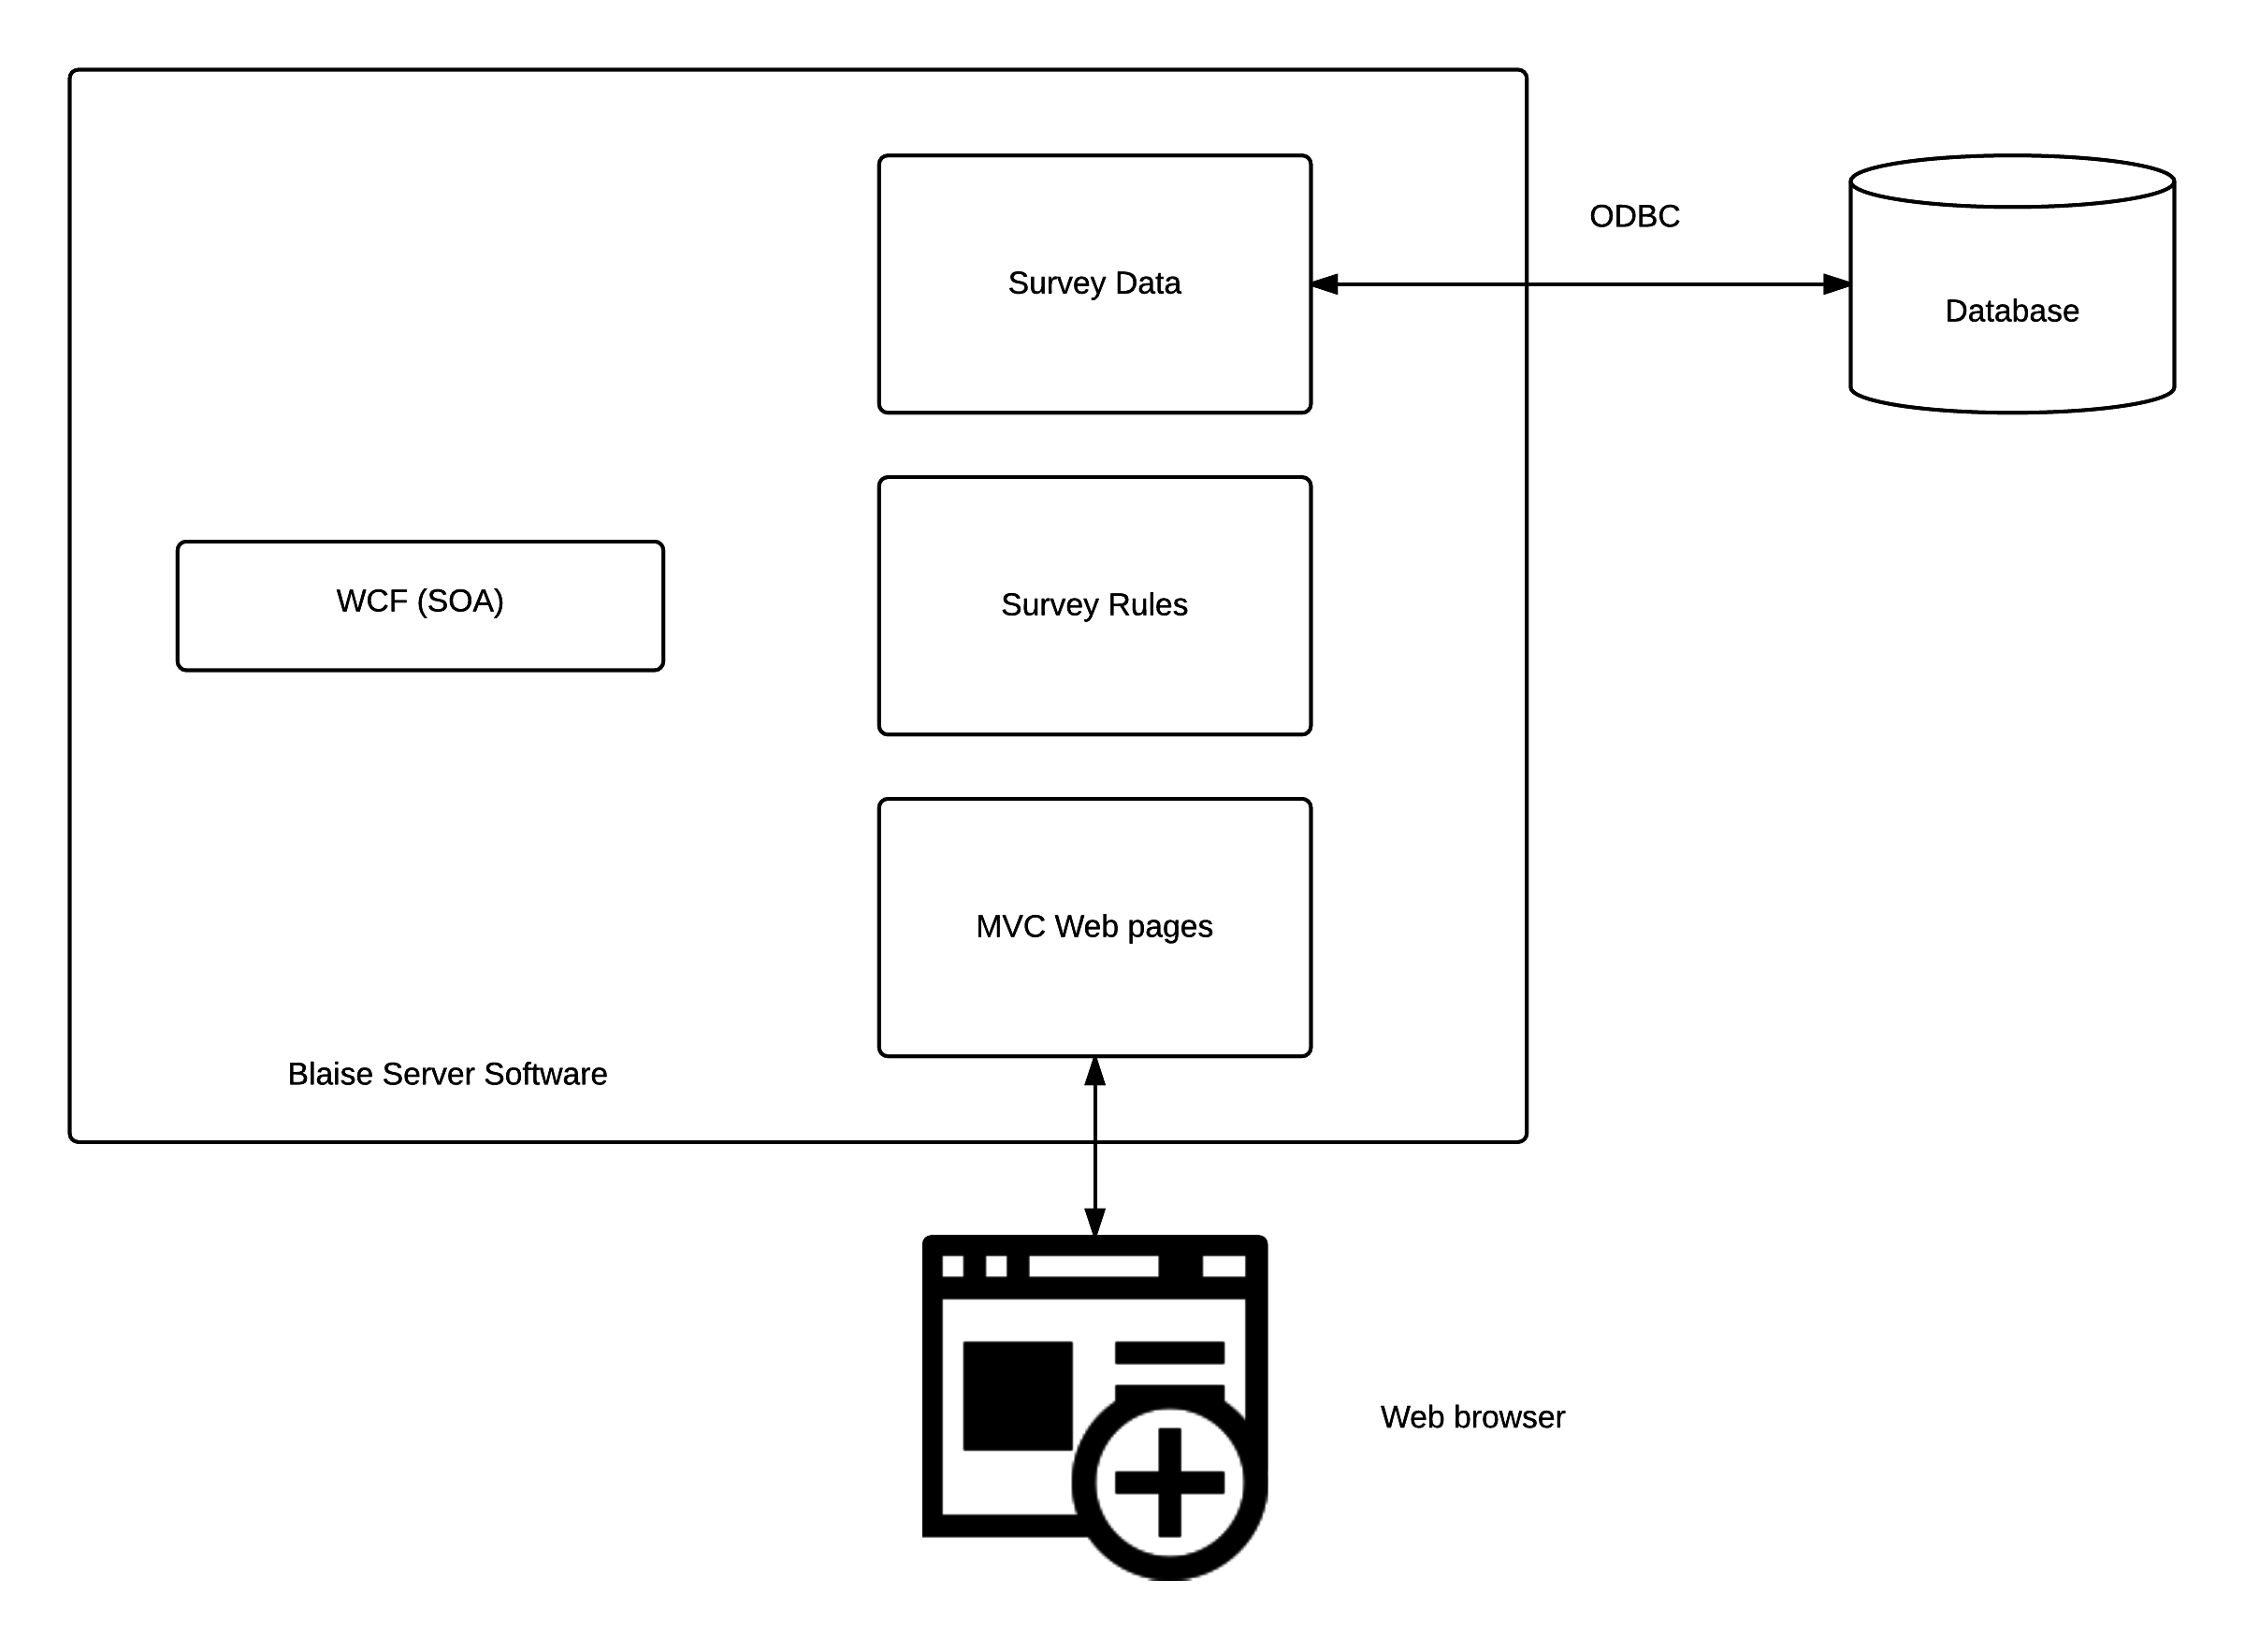
\includegraphics[max size={\textwidth}{\textheight}]{literature/img/soaBlaise.png}
	\caption{Blaise Architecture}
	\label{fig:literature:soaBlaise}
	\end{figure}

	The \gls{wcf} architecture style of Blaise induces simplicity by making a clear separation of concerns that leads to have services less complex and interdependent. Additionally, as this approach defines interfaces to communicate the different roles, any change at any component should not impact negatively into its consumers. However, the portability, reliability and scalability are not carefully considered. Specifically, the portability is not present due to the platform-dependent architecture of \gls{wcf} that only works under Microsoft environments. Regarding the reliability, it may be affected by the fact that the data server role makes the entire system vulnerable under any failure due to its inability to be set up with multiple physical or virtual machines \cite{proc:volguine13}. In respect to the scalability, the presence of a session server role to keep the state of every interview ongoing, not only prevents the server to free resources but also makes it harder to manage, replicate and synchronise state changes under a multi-server configuration.

	\subsubsection{SurveyMonkey}\label{sec:literature:surveyMonkey}
	%http://www.slideshare.net/mingli.yuan/a-brief-introduce-to-wsgi
	%http://agiliq.com/blog/2013/07/basics-wsgi/
	%https://developer.surveymonkey.com/api/v3/#authentication
	SurveyMonkey is the world's largest survey company \cite{web:groom14}. Its \gls{cawi} solution is written in Python and its core features are separated into different services. Most of the services communicate through a \gls{json} web \gls{api} over \gls{http}/\gls{http}S. SurveyMonkey implements \gls{soa} through \gls{wsgi} (see Figure \ref{fig:literature:surveyMonkey}). In this style, the web server is set up to receive client's requests and return responses back. The web server itself, does not directly creates a response but invokes the web application that produces a response based on the \gls{url} requested and pass it back to the web server. The server ultimately sends to the client. The \gls{wsgi} specifies the rules that need to be implemented by both sides, i.e. the web server and \gls{mvc} Framework. SurveyMonkey utilises Pyramid as the web application framework to produce many of its services.

	\begin{figure}[h]
	\centering
	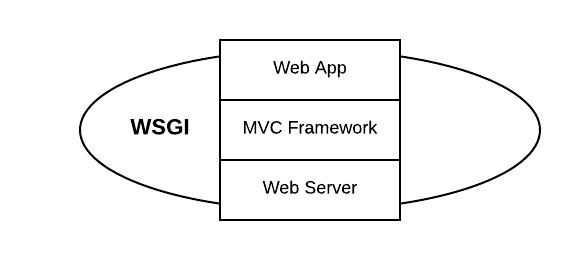
\includegraphics[width=0.75\textwidth]{literature/img/surveyMonkey.png}
	\caption{SurveyMonkey Architecture}
	\label{fig:literature:surveyMonkey}
	\end{figure}

	The \gls{wsgi} architecture style of SurveyMonkey induces simplicity and scalability. The simplicity is achieved through the use of pyramid \gls{mvc} web framework which permits loose coupling due to the separation of concerns. This software pattern, promotes parallel development (e.g. developers may focus on models, controllers or views). Regarding the scalability, unlike Blaise, there is no session persisted on the server, i.e. its stateless configuration based on a token-based authentication, promotes flexibility to scale. In respect to the portability, the application code is written in a cross-platform language, however we have not found enough information to determine whether or not the reliability or portability are induced. %For instance, the lack of awareness regarding its database solution



	\subsection{Performance Testing}\label{sec:literature:performanceTesting}
			\gls{cawi} systems are addressed for large group of respondents that can access simultaneously to complete a questionnaire at any time. As these systems are network-based applications, it is desired to conduct performance testing in order to determine the capacity of the system to work under different configurations.

	The performance testing consist of creating different test plans by varying parameters such as number of concurrent users or the complexity of the survey selected. Typically, the methodology plan to execute performance testing consist of:

	\begin{itemize}
		\item Selecting a survey, where the length and complexity helps to predict the performance of the system to deal with questionnaires with similar constructs.
		\item Designing a specific scenario either by randomly responding to questions or by taking the most common sequence of questions answered by survey respondents \cite{proc:volguine13}.
		\item Varying the number of concurrent respondents and finally running the scenario under the parameters chosen.
	\end{itemize}

	Segel et al. discuss a \emph{stress test} strategy in order to verify the capacity of a web deployment of Blaise system \cite{proc:segel13}. In that experiment, they vary the number of concurrent respondents and introduce the \emph{thinking time} concept consisting of setting up a random distributed time that simulates the amount of time that takes respondents to answer questions. Additionally, they explain the importance of selecting an adequate time in which the maximum number of concurrent users will be reached in order to avoid unrealistic simultaneous accesses.

	A more recent study carried out by Volguine pursues a stable and responsive on-line survey respondent experience through the introduction of three more test strategies a part from stress testing. These are: \emph{normal capacity} consisting in monitoring the system for two hours under an average load level for a day, \emph{peak} during two hours under a maximum load expected for day and \emph{endurance} with a significant load level during eight hours \cite{proc:volguine13}. Although Volguine offers a full suite of tests to assess performance, reliability and responsiveness of Blaise, it is not clear whether the thinking time is included or not. Therefore, this can lead to a biased testing situation that is not close to a real scenario in which an interviewee thinks before responding to a question. Moreover, the use of normal, peak and endurance tests strategies assumes that the tester knows what are the system level usages which is not always known, specially for \gls{cawi} systems that have never been in the market.

\section{Conclusions}
		Our \gls{cawi} system solution for survey life-cycle adopts \gls{rest} constraints to adhere to scalability, simplicity and reliability architectural properties expected for \gls{cawi} systems. Particularly, the \gls{rest} \gls{api}, which conforms to the \gls{http} protocol, has been implemented with the standard reference library for Java. This multi-layered solution is highly portable and uses a \gls{nosql} database solution which permits a more flexible persistence solution when compared to the traditional relational databases.

	The client side, based on the \gls{spa} not only improves the responsiveness of a distributed system but also helps to produce richer interactive interfaces. This paradigm when compared to the multi-page approach that \gls{cawi} systems such as Blaise or SurveyMokey adopt, is more attractive. Particularly, with the choice of AngularJS as the framework for building pages, we have gained a simplified cross browser testing of functionalities, reduced the server burden by transferring interface logics to the client and promoted a parallel development of design and collection interfaces.






\chapter{CAWI Mark-up Language}\label{ch:cawiLanguage}	
			This Chapter presents \gls{cawiml} as an alternative authoring language to specify questionnaires only using standard \gls{xml} schema languages. Particularly, it uses a state-transition paradigm for question's sequence and is intended to facilitate the questionnaire routing logic more adequately than the popular hierarchical model. \gls{rpn}, is the expression formalism utilised for describing routing and personalisation constructs indistinctly.

	The rest of this Chapter is structured as follows: Section \ref{sec:cawiLanguage:stateTransition} introduces the state-transition routing structure. Section \ref{sec:cawiLanguage:rpn} explains the postfix notation mode as the formalism for questionnaire expressions, followed by Section \ref{sec:cawiLanguage:xmlLanguage} that explains our \gls{xml} authoring solution. Finally, \gls{xml} details for content, routing and personalisation constructs expressed in \gls{cawiml} are presented in Section \ref{sec:cawiLanguage:cawiml}.
	\section{The State-Transition Modelling Solution}\label{sec:cawiLanguage:stateTransition}
			The state-transition modelling approach is our proposal to better address the routing requirements involving design-code equivalence and adaptability criteria (see Section \ref{sec:literature:flowParadigm}). This model, widely used for the specification of reactive systems \cite{tech:androutsopoulos08}, is inspired by the \gls{efsm} \cite{book:alagar11}.

	An example of the state-transition model, represented in Figure \ref{fig:design:stateTransition}, describes the questionnaire presented in Figure \ref{fig:background:survey}. It contains various types of states, represented by ellipses, that are linked through transitions to form state models (e.g. the Outer and Inner rectangles). 

	Each state model contains variables that reference questions defined in a section (e.g. INF1, Q1, Q2, Q3, Q4, Q5, INF2 and END for the Outer section or Q6a for the Inner). The scope of these is local to a state model and therefore their references do not exist outside. In order to reference variables through any state model, this paradigm defines global place holders, known as fields, that permit sharing data across different parts of a questionnaire (e.g. HAD\_CAR describing an integer number of cars that the respondent had).

	The states are addressed to perform single operations and these may be categorised as follows:

	\begin{itemize}
		\item \emph{Simple} states are used to present the questions to the respondent and to store responses in variables (e.g. every state prefixed with 's').
		\item \emph{Composite} states refer to a defined state model (e.g. c0 and c1 for Outer and Inner state models respectively) and are useful for reducing coupling among questions in a survey.
		\item Pseudo states are normally used to take routing path decisions through the evaluation of boolean expressions. Specifically, there are \emph{if} and \emph{for} states to decide the conditions under which questions are asked and \emph{check} states to validate inconsistent responses. Additionally, the \emph{computation} state unlike its counterparts is utilised to update place holder variables through \emph{arithmetic} expressions.
	\end{itemize}

	The transitions connect a state source with a state target to create a questionnaire's flow (e.g. arrows connect ellipses). If a transition does not define a boolean expression, it is assumed true whenever the state source of the transition is reached. In contrast, if a boolean expression is defined, this means that the expression has to be evaluated in order to determine its truth (e.g. Q1 '01' IS\_SEL Q1 '02' IS\_SEL OR Q1 '03' IS\_SEL OR). Here we propose the use of postfix notation mode as the expression formalism for all the expressions used in the design of a questionnaire.

	The state models have an initial state that determines what state is executed first (e.g. s0 and s8 for Outer and Inner respectively) as well as one or more ending states (e.g. 'sink0', 'sink1' or 'sink2'). Similarly, the state-transition model requires a state model that marks the beginning, i.e. an entry point for the model to capture a questionnaire's flow (e.g. 'c0' and 'sink0' states).

	%Our model reacts to a two types of events: \emph{external}, which occurs whenever a respondent requests moving forward or backward through a questionnaire; and \emph{internal} that is triggered every time a variable is updated. This updating forces an automatic re-evaluation of every expression that contains a reference to that variable. This is possible as X adopts the Observer pattern design implementation. %(see Appendix \ref{sec:design:observerPattern}).

	Accordingly, we formalise the state-transition model that is applied to questionnaire routing as follows:

	\begin{equation}\label{design:eqn:stateTransition}
		M = \langle Q,V,T,I,E \rangle
	\end{equation}
	where,
	\begin{enumerate}
		\item $Q(\neq \emptyset)$ is a finite set of states.
		\item $V$ is the set of state variables. Every variable $x \in V$ may be accessed at every state $q \in Q$.
		\item $T$ is a finite set of transitions. A transition $t \in T$ is represented as $q \xrightarrow{[c]} 
		q'$, where $\{q,q'\} \in Q$ and c is a boolean expression involving variables of $V$ defined in pre-state \emph{q}. The absence of $c$ is interpreted to true.
		\item $I\subset Q$ is the set of initial states. Every composite state has an initial state and consequently there is a set of initial states if the model contains composite states.
		\item $E\subset Q$ is the set of end states. These states may be \emph{sink} addressed to finish a state model or \emph{terminate} to interrupt and finish the execution of a state-transition model.
	\end{enumerate}

	\begin{figure}[H]
	\centering
	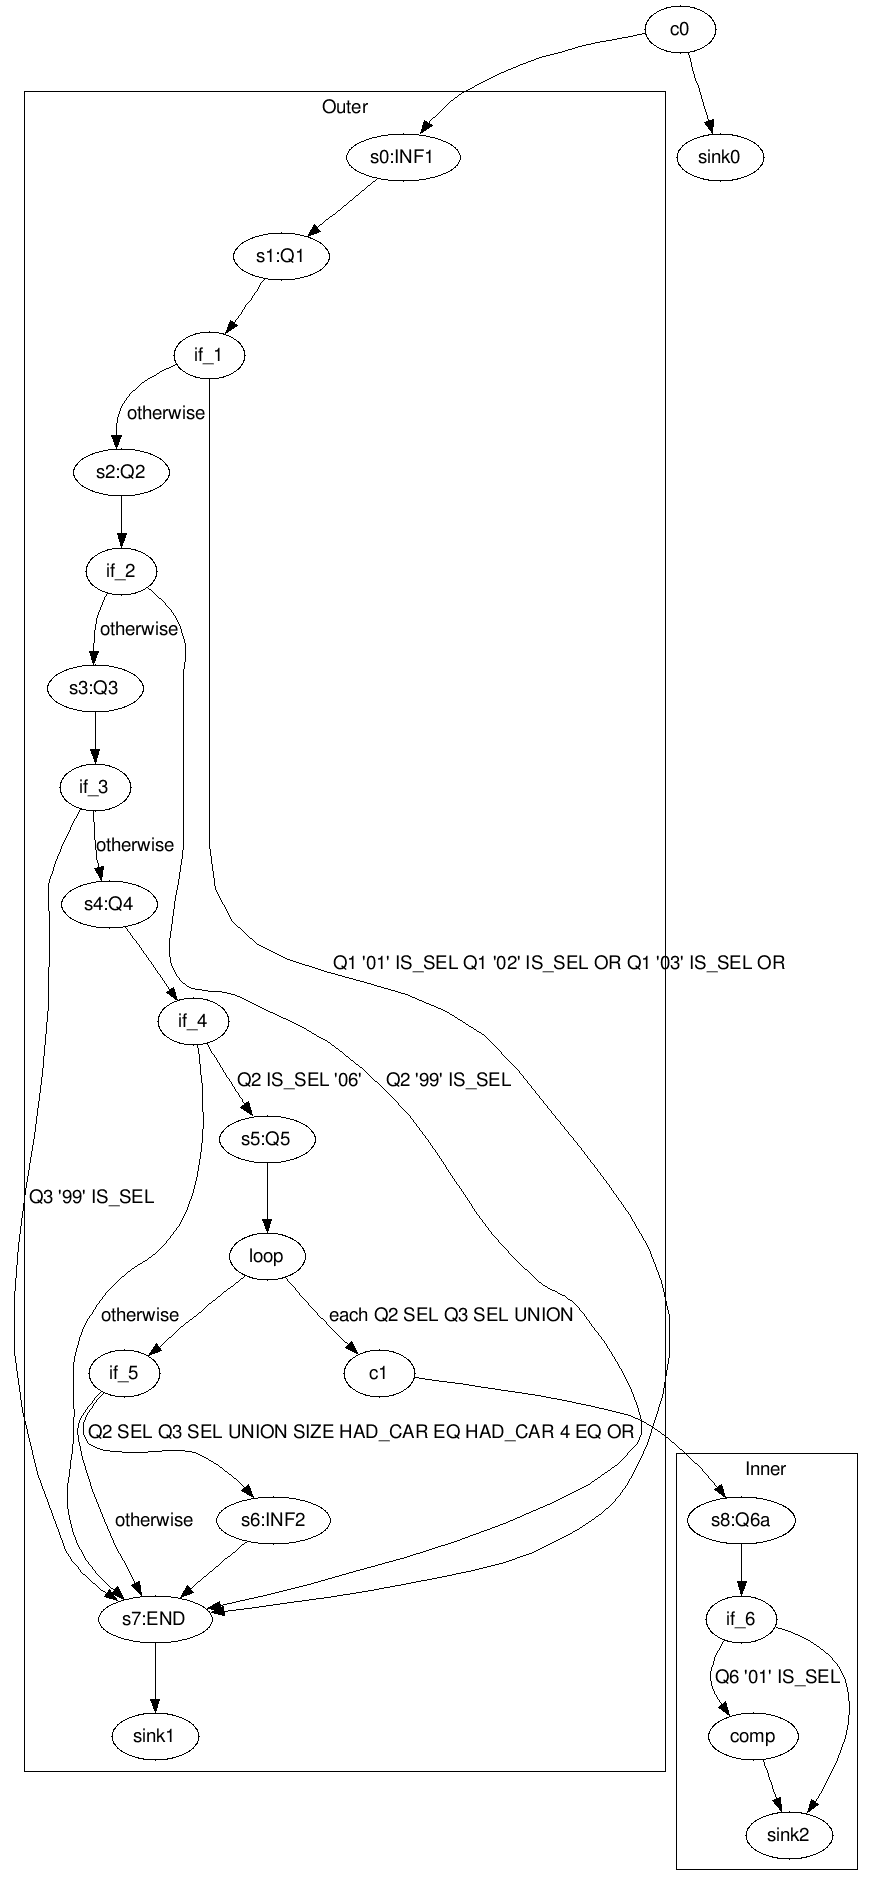
\includegraphics[max size={\textwidth}{\textheight}]{design/img/stateTransition.png}
	\caption{State-Transition for the paper questionnaire in Figure \ref{fig:background:survey}}
	\label{fig:design:stateTransition}
	\end{figure}

	%Our proposal for modelling questionnaire's routing does not explicitly defines skip constructs but it does not mean that the task of negating expressions has to be performed since this model does not rely on sequence lines which allows moving from one state to another by using transitions. Also as there is no possibility to define parent-child hierarchies among states, this potentially reduces the coupling of the routing constructs.

	





	\section{The RPN Notation}\label{sec:cawiLanguage:rpn}
		    The postfix notation, also known as \gls{rpn}, is the notation formalism that we have adopted to define the logical and arithmetical expressions applicable not only for routing constructs such as filters, loops, checks and computations but also for describing text-fill and carry-forward personalisation constructs. Its simplicity to evaluate any kind of expression, the non-ambiguity for operators precedence and its efficiency in terms of number of operations to perform, make this formalism significantly better than infix or prefix modes (see Section \ref{sec:literature:expressionNotation}). The \gls{rpn} formalism has two types of operations: \emph{unary}, that expect one and only one operand; and \emph{binary} which require two operands. By combining these two categories, it is possible to express from simple to complex questionnaire logic constructs.

    Table \ref{tab:design:rpnunary} lists the set of unary operators that \gls{cawiml} provides to express typical questionnaire constructs. The last four operators (e.g. \emph{SEL}, \emph{UNSEL}, \emph{ALL} and \emph{VALUEOF}) are particularly useful for operations carried out through piping constructs. For instance, Figure \ref{fig:background:survey} specifies a carry-forward piping to populate the unselected answers for Q2 as part of responses for Q3 (e.g. Q2 UNSEL). Similarly, the example questionnaire describes a text-fill construct for the Q6a text. This piping feature, which may be formally expressed as ITERATOR VALUEOF, describes the current loop iterator value since Q6a may be executed multiple times during the process of conducting an interview.

    \begin{table}
    \begin{center}
    \begin{tabular}{|c|c|c|}
    \hline 
    \textbf{Name} & \textbf{Operand 1} & \textbf{Result}\tabularnewline
    \hline 
    \hline 
    \textbf{POS} & Integer/Decimal & Integer/Decimal\tabularnewline
    \hline 
    \textbf{NEG} & Integer/Decimal & Integer/Decimal\tabularnewline
    \hline 
    \textbf{INC} & Integer & Integer\tabularnewline
    \hline 
    \textbf{DEC} & Integer & Integer\tabularnewline
    \hline 
    \textbf{NOT} & Boolean & Boolean\tabularnewline
    \hline 
    \textbf{EMPTY} & String/List & Boolean\tabularnewline
    \hline 
    \textbf{SIZE} & String/List & Integer\tabularnewline
    \hline 
    \textbf{SEL} & List & List\tabularnewline
    \hline 
    \textbf{UNSEL} & List & List\tabularnewline
    \hline 
    \textbf{ALL} & List & List\tabularnewline
    \hline 
    \multirow{4}{*}{\textbf{VALUEOF}} & String & \multirow{4}{*}{String}\tabularnewline
    \cline{2-2} 
     & Integer & \tabularnewline
    \cline{2-2} 
     & Decimal & \tabularnewline
    \cline{2-2} 
     & List & \tabularnewline
    \hline 
    \end{tabular}
    \caption{Unary Operators of CAWIML}
    \label{tab:design:rpnunary}
    \end{center}
    \end{table}

    The set of binary operator constructs are listed in Table \ref{tab:design:rpnbinary} and differentiates the operations into four subtypes:
    \begin{itemize}
        \item \emph{equality and relational}, used for conditional statements such as filter, loop or check;
        \item \emph{conditional}, utilised to join two boolean expressions;
        \item \emph{arithmetical}, for operations such as addition, subtraction, multiplication or division; and
        \item \emph{list} to perform operations like UNION or INTERSECTION of sets.
    \end{itemize}

    The commonly used binary operator \emph{IS\_SEL}, checks whether or not a response from a single, multiple or grid question has been chosen. Operators such as UNION or INTERSECTION are crucial to express personalisation features such as complex carry-forward constructs as these permit the join of selected, unselected or all responses from different question types (like single or multiple).

    \begin{sidewaystable}
    \begin{center}
    \begin{tabular}{|c|c|c|c|c|}
    \hline 
    \textcolor{blue}{Type} & \textcolor{blue}{Name} & \textcolor{blue}{Operand 1} & \textcolor{blue}{Operand 2} & \textcolor{blue}{Result}\tabularnewline
    \hline 
    \hline 
    \multirow{7}{*}{\textcolor{blue}{Equality and Relational}} & \multirow{2}{*}{\textbf{EQ}} & String & String & Boolean\tabularnewline
    \cline{3-5} 
     &  & Integer/Decimal & Integer/Decimal & Boolean\tabularnewline
    \cline{2-5} 
     & \multirow{2}{*}{\textbf{NE}} & String & String & Boolean\tabularnewline
    \cline{3-5} 
     &  & Integer/Decimal & Integer/Decimal & Boolean\tabularnewline
    \cline{2-5} 
     & \textbf{LT} & Integer/Decimal & Integer/Decimal & Boolean\tabularnewline
    \cline{2-5} 
     & \textbf{LE} & Integer/Decimal & Integer/Decimal & Boolean\tabularnewline
    \cline{2-5} 
     & \textbf{GT} & Integer/Decimal & Integer/Decimal & Boolean\tabularnewline
    \hline 
    \multirow{2}{*}{\textcolor{blue}{Conditional}} & \textbf{OR} & Boolean & Boolean & Boolean\tabularnewline
    \cline{2-5} 
     & \textbf{AND} & Boolean & Boolean & Boolean\tabularnewline
    \hline 
    \multirow{5}{*}{\textcolor{blue}{Arithmetical}} & \textbf{ADD} & Integer/Decimal & Integer/Decimal & Integer/Decimal\tabularnewline
    \cline{2-5} 
     & \textbf{SUB} & Integer/Decimal & Integer/Decimal & Integer/Decimal\tabularnewline
    \cline{2-5} 
     & \textbf{MUL} & Integer/Decimal & Integer/Decimal & Integer/Decimal\tabularnewline
    \cline{2-5} 
     & \textbf{DIV} & Integer/Decimal & Integer/Decimal & Integer/Decimal\tabularnewline
    \cline{2-5} 
     & \textbf{MOD} & Integer & Integer & Integer\tabularnewline
    \hline 
    \multirow{3}{*}{\textcolor{blue}{List}} & \textbf{IS\_SEL} & List & String & Boolean\tabularnewline
    \cline{2-5} 
     & \textbf{UNION} & List & List & List\tabularnewline
    \cline{2-5} 
     & \textbf{INTERSECTION} & List & List & List\tabularnewline
    \hline 
    \end{tabular}
    \caption{Binary Operators of CAWIML}
    \label{tab:design:rpnbinary}
    \end{center}
    \end{sidewaystable}
   

	\section{The XML Language Solution}\label{sec:cawiLanguage:xmlLanguage}
			The limitations for all grammar-based \gls{xml} language solutions reviewed (see Section \ref{sec:literature:schemaLanguages}) require the use of programming languages to validate semantics for questionnaire specifications. These restrictions have led us to design and implement a new authoring language that is non-proprietary, platform independent and use standard formalisms to define structure, data-types, integrity constraints and business rules. This language, uses the state-transition model for routing logic (see Section \ref{sec:cawiLanguage:stateTransition}) together with \gls{rpn} notation to define expressions either for routing or personalisation constructs (see Section \ref{sec:cawiLanguage:rpn}).  

	\gls{cawiml} uses \gls{xsd} to define structure and data types together with \gls{sch} to express integrity constraints and business rules. We have chosen \gls{xsd} due to its well-defined patterns to express vocabulary and structures, its rich set of data-types, its use of \gls{xml} to define constraints and because it is the recommendation schema formalism proposed by \gls{w3c} (see Section \ref{sec:background:xsd}). \gls{sch} adheres to standard \gls{iso}/\gls{iec} 19757 and is also the only rule-based schema language known to address the semantics limitations that grammar-based languages have through XPath query language (see Section \ref{sec:background:sch}). Therefore, to ensure the correctness of \gls{xml} questionnaire instances, we employ a two step process to integrate four different levels of validation. Figure \ref{fig:design:xmlValidation} describes how this process is carried out.

	\begin{figure}[h]
	\centering
	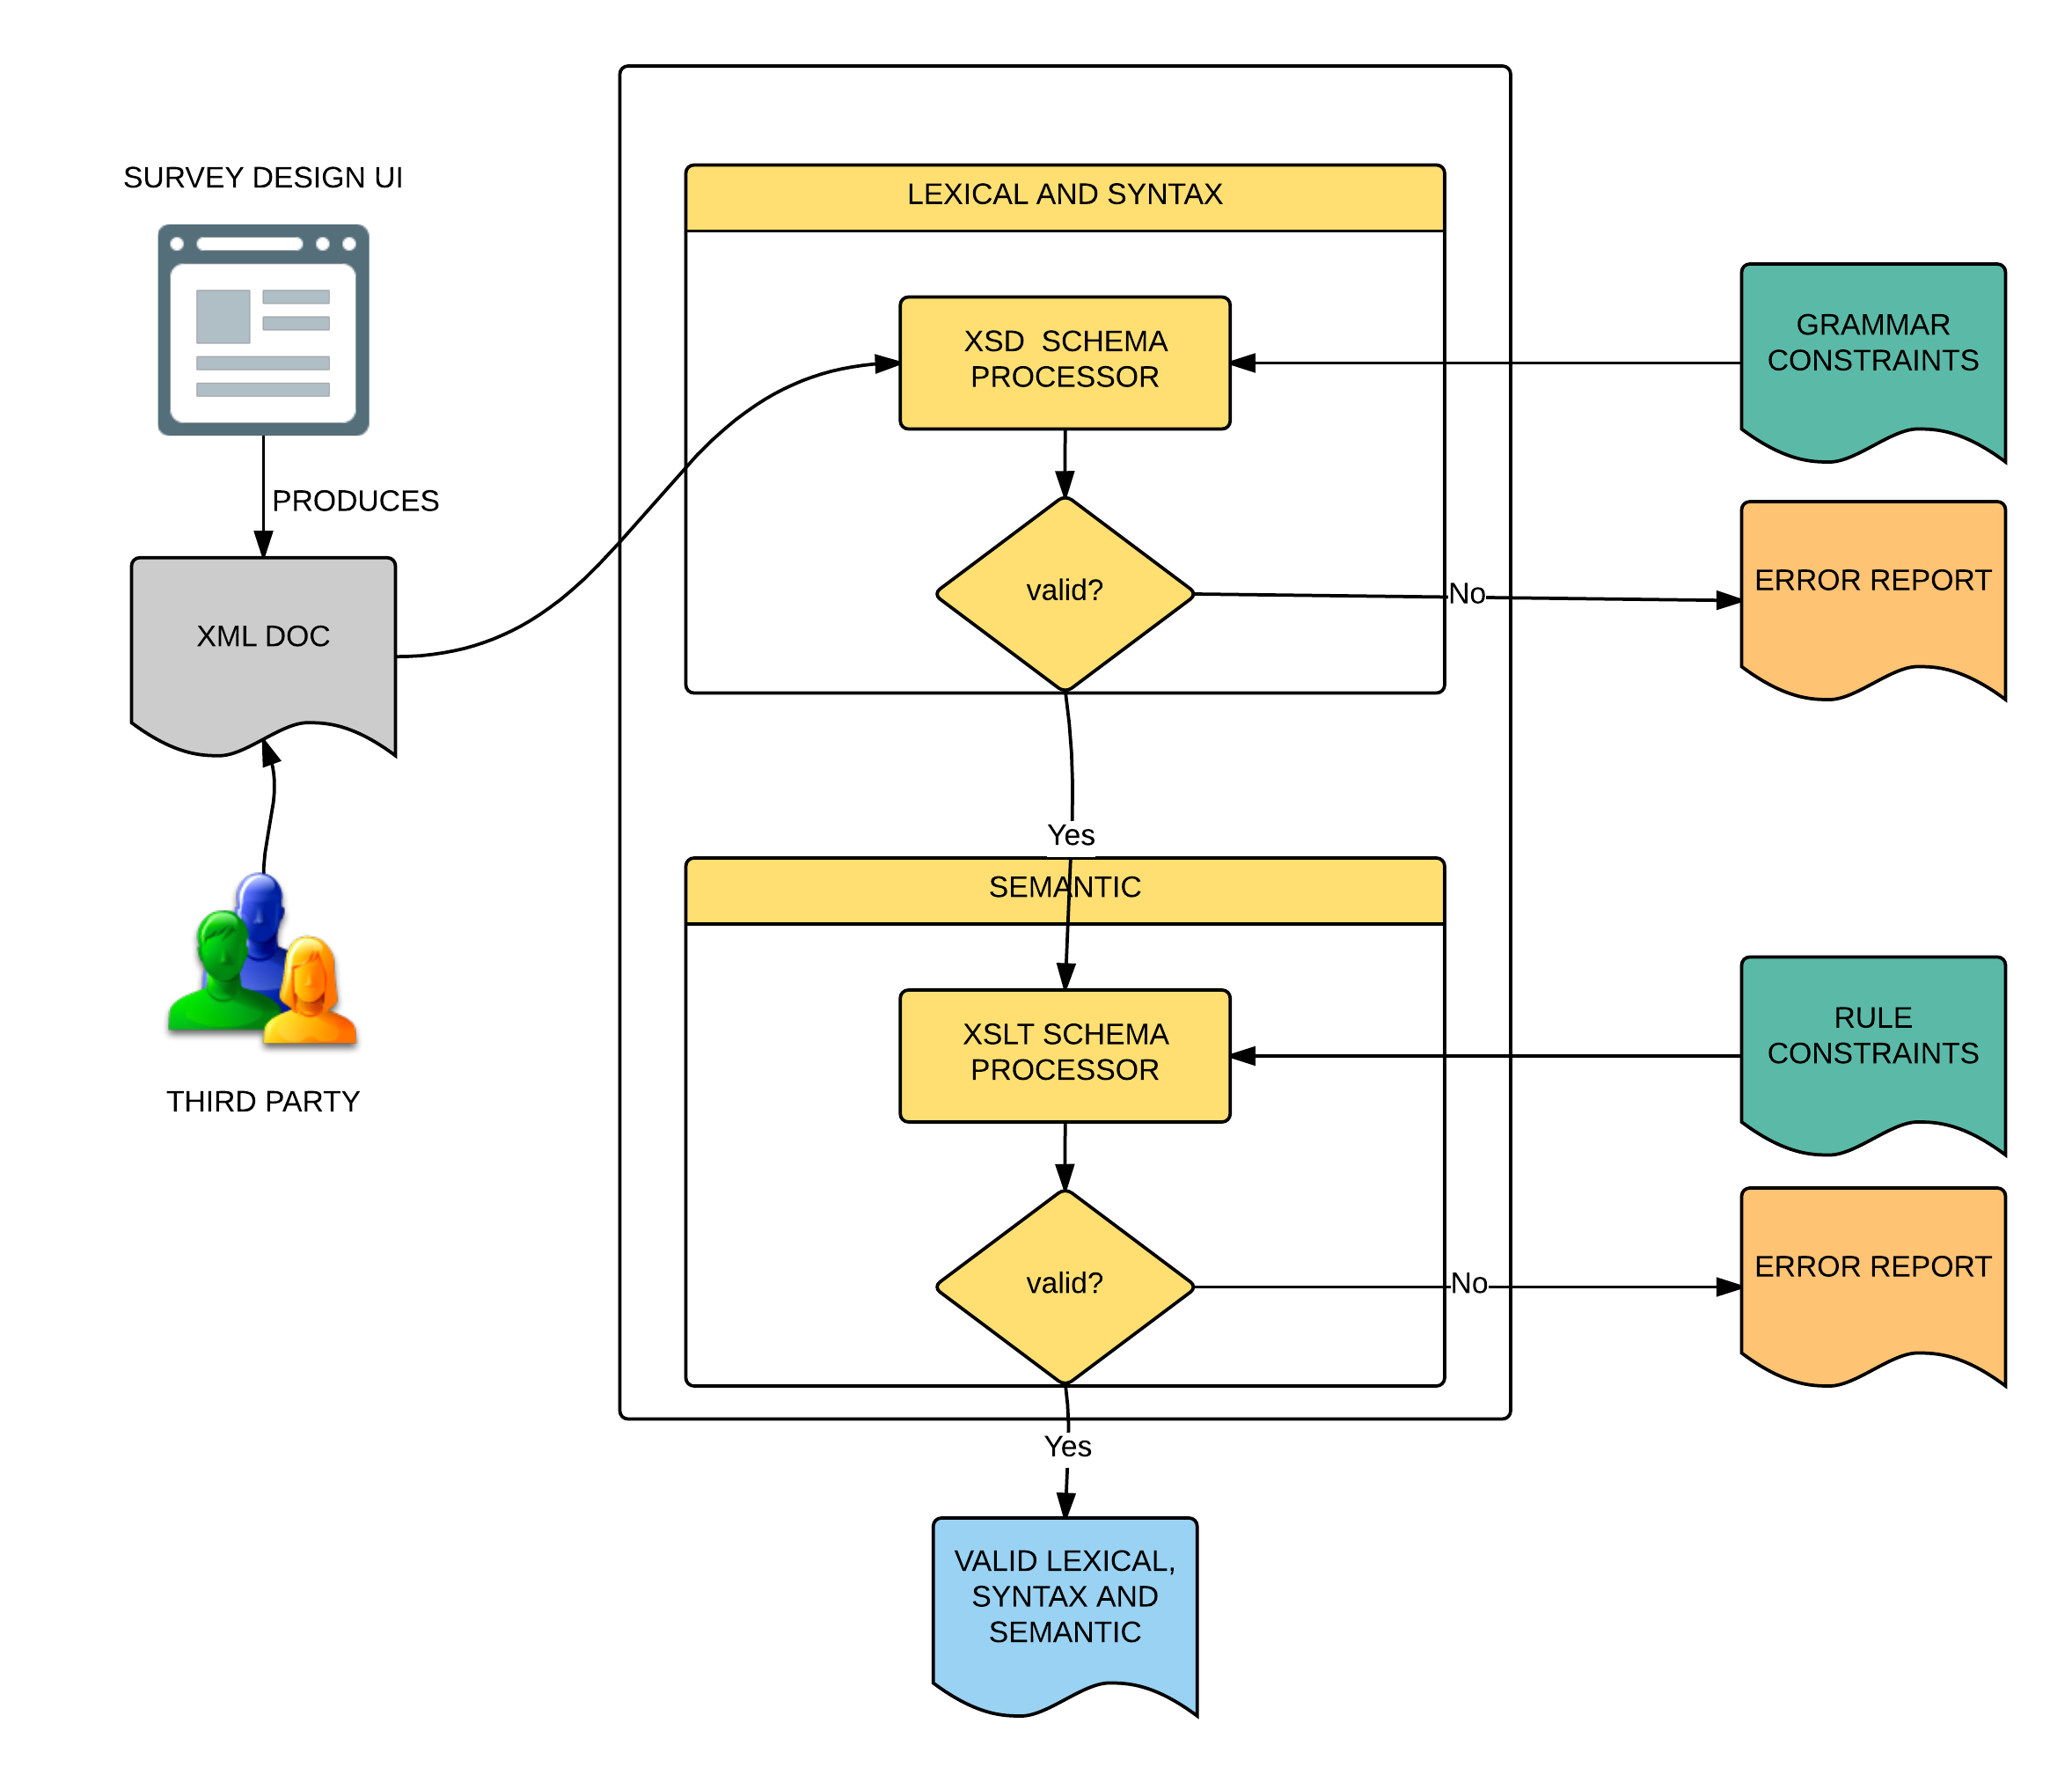
\includegraphics[max size={\textwidth}{\textheight}]{design/img/xmlValidation.png}
	\caption{Validation process of CAWIML}
	\label{fig:design:xmlValidation}
	\end{figure}

	An \gls{xml} document, that is presented either from our interface for designing questionnaires or from any third party, is passed to the validation component. In the first instance, the \gls{xml} schema processor takes our grammar constraints and an \gls{xml} document to verify whether the vocabulary, structures and data-types are valid. Two types of errors can arise from this operation, \emph{non-recoverable} errors that halt the process, i.e. the document is not well-formed (see Section \ref{sec:background:xml}) or \emph{recoverable} which are queued without interrupting the \gls{xml} processing.

	In the second instance, an \gls{xslt} processor takes our \gls{sch} rules, previously converted to the valid format accepted from this processor (see Section \ref{sec:background:sch}), and the \gls{xml} document to determine whether or not the relationships and domain specific rules are correct. The absence of any error at this stage confirms that the \gls{xml} document is valid according to our structure, data-types, integrity constraints and business rules and it is consequently ready to be parsed in our \gls{cawi} system for conducting the on-line survey.

	%We have found during the implementation that the reporting of errors is significantly less predictable for the the grammar-rules since \gls{xsd} schema only produces messages suited for debugging purposes \cite{masterthesis:madsen09}, being difficult to understand for people without any knowledge on schema languages. In contrast, \gls{sch} schema has permitted us to define customised messages that are more user-friendly and better suited for production environments.

	




	\section{CAWIML Language Details}\label{sec:cawiLanguage:cawiml}
			\gls{cawiml} addresses the content, routing and personalisation constructs of surveys by structuring \gls{xml} documents into 5 categories:

	\begin{enumerate}
		\item \emph{Survey} element defines global information relative to a questionnaire and contains information such as name, description and date.
		\item \emph{Content} specifies questions grouped through sections. It provides support for the common question types such as intro, single, multiple, open and grid questions.
		\item \emph{Field} element defines place holders variables needed to share information across different questionnaire sections. String, integer, decimal and list are the types supported currently.
		\item \emph{Routing} captures questionnaire's flow using the state-transition structure proposed in Section \ref{sec:cawiLanguage:stateTransition}.
		\item \emph{Personalisation} defines constructs to adapt questionnaires for an interviewee through features such as text-fill, carry-forward, randomising and rotating.
	\end{enumerate}

	Listings \ref{code:impl:globalStructure} represents the necessary elements to create a specification in \gls{cawiml}. The following sections, showcase the content, routing and personalisation categories.

	\lstinputlisting[caption={CAWIML global structure},label={code:impl:globalStructure}]{appendix/code/overview.xml}


	
		\subsection{The Content Constructs}\label{sec:cawiLanguage:contentConstructs}
				The content category of \gls{cawiml} is structured in sections. A section may contain one or more questions within and it is referenced through a state model (see Section \ref{sec:cawiLanguage:routingConstructs}). Our authoring language permits describing the most common question types for questionnaires (e.g. intro, single, multiple, open and grid). Listings \ref{code:impl:content} defines two sections (e.g. Outer and Inner) within the content element to group the questions specified in Figure \ref{fig:background:survey}. Essentially the use of a section serves as a container that defines questions through which state models reference and decide question's sequence. 
	\lstinputlisting[caption={Content category},label={code:impl:content}]{appendix/code/content.xml}

	In the outer section, there are eight questions (e.g INF1, Q1, Q2, Q3, Q4, Q5, INF2, END). For instance, an open-ended integer question (e.g. Q5), defined in Listings \ref{code:impl:open}, permits asking the number of cars of brand F that the interviewee has had. The open-ended integer question offers the possibility to define boundaries (e.g. min and max elements) in which the number responded must be within. It also allows setting a default value for the first time the question is shown to the interviewee (e.g. value element).

	\lstinputlisting[caption={Open-ended question},label={code:impl:open}]{appendix/code/open.xml}

	The inner section unlike the outer, only defines one question (e.g. Q6a) whose type is single. A single question (see Listings \ref{code:impl:single}) is addressed to capture one and only one response from a set. The example provided, asks through the label element whether or not the respondent had a car from a particular brand. Note that there is a text-fill pipe reference defined within that label (see Section \ref{sec:cawiLanguage:personalisationConstructs}) which will be replaced with the specific brand once the questionnaire is executing. This single question also defines two closed responses with codes 01 and 02 for yes and no respectively.

	\lstinputlisting[caption={Single question},label={code:impl:single}]{appendix/code/single.xml}

	In order to see other question types, please refer to Appendix \ref{sec:appendix:ssmInstance} containing the definition for the questionnaire from Figure \ref{fig:background:survey} in \gls{cawiml}.
		\subsection{The Routing Constructs}\label{sec:cawiLanguage:routingConstructs}
				The routing in \gls{cawiml} is composed of different state models that reference to sections defined in the content part of the language. Throughout this section, the questionnaire from Figure \ref{fig:background:survey} will be used to discuss the features supported by \gls{cawiml}. In Listings \ref{code:impl:routing}, there are two state models (e.g. Outer and Inner) to capture the question's sequence from those sections. In addition, there is an entry point state model element that marks the beginning of the questionnaire's flow. 

	Every state model defines an initial state that determines what is the first state to execute through a source element (e.g. Outer defines INF1). Similarly, it requires at least one state that describes the end of a question's sequence through \emph{sink} element. The different states supported in our state-transition solution for questionnaires are detailed in the following subsections. %Every state type from \gls{cawiml} is defined though a common state element with an id attribute that is used in transitions to reference the source and target 

	\lstinputlisting[caption={State-transition routing},label={code:impl:routing}]{appendix/code/routing.xml}

	\subsubsection{Sink}
		Sink state is aimed at describing the ending of a state model, i.e. it marks the end of a section. For instance, Listings \ref{code:impl:sink} describes a sink with id 'sink0'. When this state is reached, the state model Outer finishes and consequently the questionnaire terminates. As the reader may appreciate, there are no outgoing transitions from this state type. 
		\lstinputlisting[caption={Sink state},label={code:impl:sink}]{appendix/code/sink.xml}

	\subsubsection{Terminate}
		Terminate state unlike Sink states, are addressed to interrupt the entire routing, i.e. when this state is reached not only finishes the state model under which is defined but also terminates the questionnaire's flow even if there are more states defined in the entry point state model. Listings \ref{code:impl:terminate} describes this state type with an id 'terminate0'.
		\lstinputlisting[caption={Sink state},label={code:impl:terminate}]{appendix/code/terminate.xml}

	\subsubsection{Simple}
		Simple state is responsible for retrieving variables, i.e. the definition of a question and its associated responses, if any. It has capabilities to define one or more variables, i.e. every variable referenced here must be presented on the same screen of the \gls{cawi} collection stage that supports \gls{cawiml}. Listings \ref{code:impl:simple} describes two simple states (e.g. INF1 and Q1) that contain references to variables (e.g. INF1 and Q1 for intro and single question respectively). For instance, when an interviewee decides to move forward through the questionnaire after reading INF1, the state Q1 is reached given the transition target defined within the INF1 state.
		\lstinputlisting[caption={Simple state},label={code:impl:simple}]{appendix/code/simple.xml}
	\subsubsection{Composite}
		Composite state permits switching to another state model. For instance, the Inner state model referenced under the 'c1' state (see Listings \ref{code:impl:composite}) describes the sequence of questions for the Inner section of the paper questionnaire that corresponds to Q6a (see Figure \ref{fig:background:survey}). Note that this state has been defined within the state model Outer, i.e. the Inner state model will be only reached under the sequence defined for the Outer state model.
		\lstinputlisting[caption={Composite state},label={code:impl:composite}]{appendix/code/composite.xml}
	\subsubsection{If-then-else}
		If state represents filter and skip constructs indistinctly. It is composed of a boolean expression in \gls{rpn} notation and describes two transitions, then and else, for true and false result of the expression respectively. For instance, Listings \ref{code:impl:ifThenElse} specifies the skip features attached over Q1, i.e. if response 01, 02 or 03 is selected, the 'sink0' state has to be reached, otherwise the interviewee will see question Q2 on the screen.
		\lstinputlisting[caption={If-then-else state},label={code:impl:ifThenElse}]{appendix/code/ifThenElse.xml}
	\subsubsection{Check}
		Check state defines a boolean expression that validates the presence of an inconsistency. There are two types supported: \emph{warning}, that alerts the interviewee but permits her to continue the section sequence; and \emph{error}, that stops the execution of the state model until the conflict is solved. Listings \ref{code:impl:check} describes a case where the questionnaire's flow is interrupted if the response was not selected. This example is useful to validate whether or not people younger than eighteen have never been married. It should described together with an if-then-else state to filter those interviewees with age under eighteen.
		\lstinputlisting[caption={Check state},label={code:impl:check}]{appendix/code/check.xml}
	\subsubsection{For}\label{sec:impl:for}
		For state captures the loop construct of surveys and similar to the if-then-else state, has two transitions one for executing the loop body and another that is reached whenever the boolean expression is not met. There are three loop types: \emph{range}, that iterates numbers by specifying start, end and step expressions (e.g. start at 0, end at 5 and step 1 would iterate from 0 to 4); \emph{List} mode, that iterates all the elements of a list defined in the field section; and \emph{expr\_list} that iterates a list returned by \gls{rpn} expression.
		
		Listings \ref{code:impl:for} describes the instruction specified over Q6a through expr\_list loop mode. This state contains: \emph{field} element, that references a global variable (e.g. 'p4\_iterator'), updated every time the iterator changes; and two transitions, one for switching to another state model (e.g. target 'c1') and the other that is reached when the loop condition is not met (e.g. target 'p5'). Note that this example includes a randomising construct (see Section \ref{sec:impl:Randomising}) that alters the iterator order and ensures that at maximum four times the loop is executed.
		\lstinputlisting[caption={For state},label={code:impl:for}]{appendix/code/for.xml}
	\subsubsection{Computation}
		Computation state is used to update place holder variables. These variables are typically used to share data across sections. For instance, Listings \ref{code:impl:computation} permits aggregating data from different state models through the global variable HAD\_CAR. This construct, implicitly defined within the paper questionnaire must be used together with an if-then-else to decide whether or not the interviewee responded \emph{yes} to the Q6a. Note that this question may be repeated multiple times for each brand mentioned at Q2 or Q3 and therefore through HAD\_CAR is captured the number of cars that the interviewee had.
 		\lstinputlisting[caption={Computation state},label={code:impl:computation}]{appendix/code/computation.xml}
	
		\subsection{The Personalisation Constructs}\label{sec:cawiLanguage:personalisationConstructs}
				The personalisation constructs in \gls{cawiml} define the dynamic behaviour for surveys. These features, that may serve to adapt the survey for each respondent, are defined in this questionnaire language through elements such as pipe, randomising and rotating. The following subsections detail the personalisation constructs through features extracted From Figure \ref{fig:background:survey}.

	\subsubsection{Text-fill piping}
		Text-fill piping describes the behaviour of retrieving responses from previous questions as part of the text for another. For instance, in Listings \ref{code:impl:textFill} a reference to a pipe (e.g. pipe0) is described as part of the text for Q6a. This pipe, defined within a piping element points at the Inner state model and has a \gls{rpn} expression describing the current loop iterator value. Note that this value may be one of the entire set of response codes from Q2 or Q3 (e.g. A, B, C, D, E, F, G, H). For instance, if the response was A for question Q2 and B,C for question Q3, the Q6a would be repeated three times by changing the pipe value to A, B or C in its question label.
		\lstinputlisting[caption={Text-fill},label={code:impl:textFill}]{appendix/code/textFill.xml}
	\subsubsection{Carry forward piping}
		Carry-forward unlike its counterpart, is intended to capture the behaviour of populating responses for a question based on a \gls{rpn} expression that returns a list. That list commonly represents the responses selected/unselected from previous questions. For instance, Listings \ref{code:impl:carry-forward} has a multiple question (e.g. Q3) that contains a pipe reference (e.g. 'pipe0'). This pipe describes the unselected responses from Q2. The \gls{cawi} system must retrieve on real-time those unselected responses to automatically populate them as part of the responses for Q3 when the gathering of survey responses takes place. For instance, if the interviewee responded A for Q2, Q3 would be automatically populated with the responses B, C, D, E, F, G, H and Don't know, that represent those non-selected at Q2.
		\lstinputlisting[caption={Carry-forward},label={code:impl:carry-forward}]{appendix/code/carryForward.xml}
	\subsubsection{Randomising/Rotating}\label{sec:impl:Randomising}
		Randomising and rotating constructs are used to alter the data order presented to the respondent. In \gls{cawiml} these features are usually defined when a question is specified but they can also be utilised for reordering loops. There are two modes of specifying data order to both randomising and rotating: 
		\begin{itemize}
			\item \emph{All} that performs ordering of the entire set of responses and contains an attribute \emph{present} to determine the number of elements to show. For instance, the for state (see section \ref{sec:impl:for}) describes this construct to alter the iterator order and determine the maximum number of times that this loop should be repeated.
			\item \emph{Subset} which selects the elements to be randomised or rotated. Listings \ref{code:impl:randomising} defines a subset of codes (e.g. 01, 02, 03, 04, 05, 06, 07 and 08) that must be reordered randomly. Note that response 09 is not included in that set and therefore this response must appear as last choice to select for Q2. 
		\end{itemize}

		The importance of having two modes arises due to the fact that sometimes there can be responses in which their order should not be modified. For instance, it is frequent to offer responses such as don't know or not applicable at last in order to capture those interviewees that really do not know enough to have a formed opinion. For that purpose, the subset construct ensures that those responses out of the subset will remain unaltered.

		\lstinputlisting[caption={Randomising},label={code:impl:randomising}]{appendix/code/randomising.xml}

	\section{Conclusions}\label{sec:cawiLanguage:conclusion}
			Our \gls{cawi} system solution for survey life-cycle adopts \gls{rest} constraints to adhere to scalability, simplicity and reliability architectural properties expected for \gls{cawi} systems. Particularly, the \gls{rest} \gls{api}, which conforms to the \gls{http} protocol, has been implemented with the standard reference library for Java. This multi-layered solution is highly portable and uses a \gls{nosql} database solution which permits a more flexible persistence solution when compared to the traditional relational databases.

	The client side, based on the \gls{spa} not only improves the responsiveness of a distributed system but also helps to produce richer interactive interfaces. This paradigm when compared to the multi-page approach that \gls{cawi} systems such as Blaise or SurveyMokey adopt, is more attractive. Particularly, with the choice of AngularJS as the framework for building pages, we have gained a simplified cross browser testing of functionalities, reduced the server burden by transferring interface logics to the client and promoted a parallel development of design and collection interfaces.
\chapter{CAWI System}\label{ch:cawiSystem}
		This Chapter presents \gls{cawiml} as an alternative authoring language to specify questionnaires only using standard \gls{xml} schema languages. Particularly, it uses a state-transition paradigm for question's sequence and is intended to facilitate the questionnaire routing logic more adequately than the popular hierarchical model. \gls{rpn}, is the expression formalism utilised for describing routing and personalisation constructs indistinctly.

	The rest of this Chapter is structured as follows: Section \ref{sec:cawiLanguage:stateTransition} introduces the state-transition routing structure. Section \ref{sec:cawiLanguage:rpn} explains the postfix notation mode as the formalism for questionnaire expressions, followed by Section \ref{sec:cawiLanguage:xmlLanguage} that explains our \gls{xml} authoring solution. Finally, \gls{xml} details for content, routing and personalisation constructs expressed in \gls{cawiml} are presented in Section \ref{sec:cawiLanguage:cawiml}.
	\section{Architecture of the System}\label{sec:cawiSystem:architecture}
			Our proposed \gls{cawi} system uses the \gls{rest} architecture \cite{phdthesis:fielding00} to consider architectural principles such as scalability, simplicity or reliability. Through \gls{rest}, the system is constrained to produce uniform interfaces using the \gls{http} verbs (e.g. GET, POST, PUT and DELETE). This restriction permits client and server to \emph{evolve} independently. For instance, changes at any service implementation reduce or eliminate the impact produced on the client. The stateless constraint, also from \gls{rest}, requires to have a server solution that avoids keeping session state for each client. For that restriction, we have implemented a token based identifier that makes it easier to \emph{scale} our solution without needing to replicate any session data across a multi-server configuration. Reliability is improved because it eases the task of recovering from partial failures within components, connectors or data \cite{phdthesis:fielding00}.

	The system is structured to separate the \gls{cawi} services from the user interfaces (see Figure \ref{fig:design:architecture}) using \gls{json} and \gls{xml} standard exchange data formats for communication. 
	%Look at which part of the architecture is driven by CAWIML. You need to find away to illustrate that on the figure and explain it when at first mention of the figure.
	The server side is structured into different layers: 
	\begin{itemize}
		\item the \emph{\gls{api} layer} (e.g. RESTful API), that uses the \gls{http} methods defined by RFC 2616 \cite{web:fielding99} creates the communication interfaces and is the only component that is directly accessible by the client;
		\item the \emph{business layer}, used by the \gls{api}, separates the different functionalities of the system through Java packages (e.g. content, routing, personalisation) in order to promote reusability; and
		\item the \emph{data access layer}, which serves to abstract the data storage solution from the business layer, makes the system easier to maintain since this connector is centralised in one place.
	\end{itemize}

	This layered server structure induces \emph{portability}, thanks to the use of Java as the general purpose programming language that works across any platform.

	\begin{figure}[h]
	\centering
	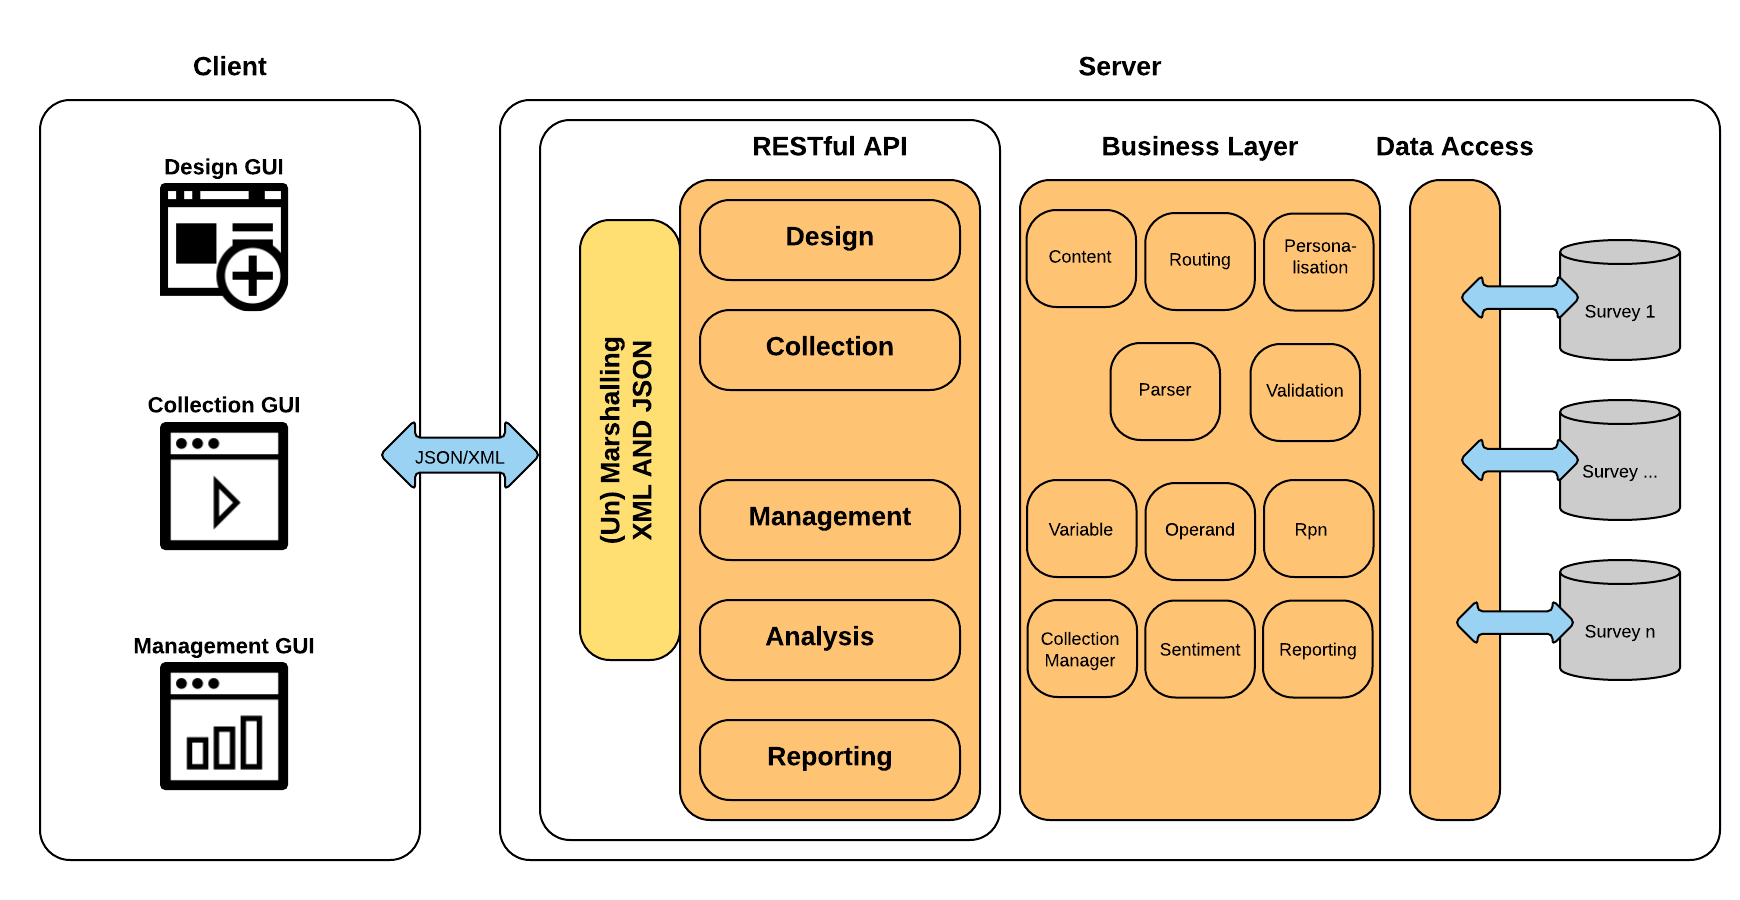
\includegraphics[max size={\textwidth}{\textheight}]{design/img/surveyArchitecture.png}
	\caption{REST architecture}
	\label{fig:design:architecture}
	\end{figure}

	The client side of this architecture makes a clear separation by building and rendering every \gls{html} code entirely on the client using the novel \gls{spa} paradigm (see Section \ref{sec:cawiSystem:spa}). This approach when compared to the multi-page paradigm, that Blaise or SurveyMonkey adopt, is more consistent with the \emph{simplicity} property, since it reduces the amount of data transferred from the server, improves user experience and reduces the burden on the server.

		\subsection{RESTful API}\label{sec:cawiSystem:restful}
				The process of conducting survey research is separated into five stages (see Section \ref{sec:literature:surveyStages}). In order to address these separated steps, we have implemented a \gls{rest} \gls{api} that permits client communication between these five services (e.g. design, collection, management, analysis and reporting). The business objects, represented as Java classes, are converted to \gls{json} or \gls{xml} every time the server responds to a request through a process named \emph{marshalling}. Similarly, when data sent from client is received, an \emph{unmarshalling} process transforms it to the adequate business object class instance.

	The design service, seen as the only stage that uses \gls{xml} exchange format to communicate the parts, deals with the definition of questionnaire instances according to \gls{cawiml}. The rest of the services, only accept \gls{json} because it offers a direct mapping to JavaScript objects in which our client interfaces are built and also it is less verbose than \gls{xml} which helps to reduce the amount of data transferred across client and server.

	The collection service uses GET, POST and DELETE \gls{http} verbs to produce uniform interfaces for communication. The GET provides services for retrieving general information of any survey (e.g. title, description or date they were created) or to fetch incomplete interviews either because the interviewer decided to postpone or because the browser was closed. The POST verb is used for actions such as starting an interview or to store questionnaire responses when moving forward and backward through a survey. The DELETE is used throughout this service for activities like marking the ending of an interview, i.e. to remove the possibility of a valid client token to modify a questionnaire that is completed.

	%The management, analysis and reporting services we have decided to implement one interface that captures all of the requirements, firstly because we still do not have enough features to clearly separate them and secondly because these stages are interdependent.

	
		\subsection{Business Layer}\label{sec:cawiSystem:businessLayer}
				The business layer, organised into different modules, is built through an object-oriented paradigm and it is used by the \gls{rest} API to retrieve or update state and behaviour. For instance, the content, routing and personalisation packages are built according to the grammatical rules that \gls{cawiml} defines in its \gls{xsd} schema. These three packages are widely used across the survey stages and following sections provide a high-level view of the different modules that are involved in each of the client stages of design, collection and management analytics.

	\subsubsection{The design stage}

	The Validation and Parser packages are crucial at the questionnaire design stage as these carry out the validation, correctness and translation of \gls{xml} constructs into artefacts that are ready for data gathering. Particularly, the parser package reads data from valid \gls{xml} specifications to produce objects according to the content, routing and personalisation modules. It uses an event-driven approach that handles a variety of small to large questionnaire specifications appropriately. The event-driven style when compared to the popular \gls{dom} parsing, uses significantly less resources since there is no need to create a tree of objects in memory representing the \gls{xml} file under process.
	%Additionally, when the parsing task is completed, routines such as the creation of Variables according to the questions (see Section \ref{sec:design:factoryPattern}) or the binding of piping features (e.g. text-fills and carry-forward) to questions are performed. Specifically, the late bindings are carried out at the end since \gls{xml} instances according to \gls{ssm} have forward references to objects that are still not created since the parser reads \gls{xml} files from top to bottom (e.g. XML FILE EXAMPLE FROM SSM).

	\subsubsection{The collection stage}

	The collection stage uses the state-transition model expressed in a \gls{cawiml} instance to conduct interviews. The class diagram from Figure \ref{fig:design:collection} represents an overview of the most important classes involved. A state model consisting of states and transitions, holds variables that represent the questions from a section and their responses. Additionally, it keeps references to pipes that together with the pseudo states, use the \gls{rpn} formalism to execute logical and arithmetical expressions. The routing class, contains a list of state models and an entry point to mark the state model execution entry point. It also holds the set of place holder variables (e.g. Field class) that are shared across state models.

	\begin{figure}[h]
	\centering
	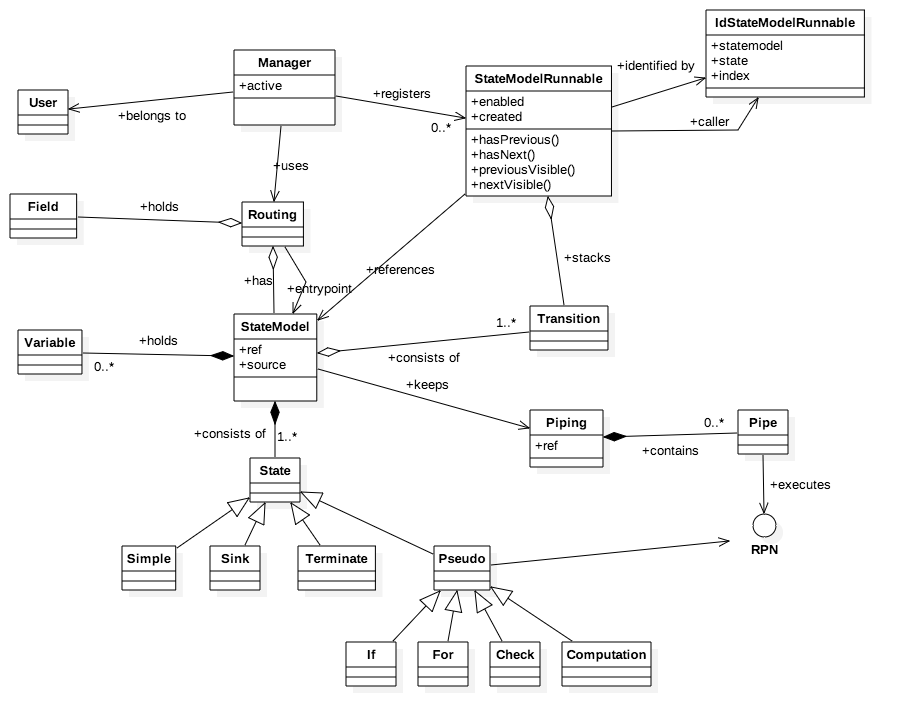
\includegraphics[max size={\textwidth}{\textheight}]{design/img/collectionManager.png}
	\caption{Class diagram for the Collection Manager}
	\label{fig:design:collection}
	\end{figure}

	Each interviewee (e.g. User class) has a Manager object that registers the set of state models defined in a state-transition and controls which state model is active at any time. The state modelRunnable class, adds behaviour to a state model by including methods such as hasPrevious(), hasNext(), previousVisible() and nextVisible() that permit navigating backward and forward through an interview. It contains interesting properties like \emph{created}, that registers the date and time in which the state model was generated, and \emph{enabled}, that determines whether or not the state model variables should be considered when data is exported or visualised on client interfaces. The instances of this class are typically identified by a state model and state (e.g. IdStatemodelRunnable) but also may contain an index if the state model is part of a loop. For instance, the inner state model from Figure \ref{fig:design:stateTransition}, that represents the questionnaire from Figure \ref{fig:background:survey}, can have up to eight different state modelRunnable instances identified by outer and 'c1' for the state model and the state respectively. Also an index that varies from 01 to 08 according to the set of response codes from Q2 or Q3 is set to identify each state model copy uniquely.

	\subsubsection{The management, analysis and reporting stages}

	The management stage, aimed at monitoring the data gathered in real time, fetches questionnaire objects by conducting multiple queries against the persistence layer. For instance, status objects are sent to the client in order to inform the percentage of completion of a questionnaire or to determine accurately the current question in an interview session.

	The analysis stage incorporate aggregate queries to study the data collection for questionnaires for each type of question. For instance, an attractive feature that calculates the degree of positivity for open string questions, automatically separates sentences into one of six categories (e.g. strong positive, positive, weak positive, weak negative, negative or strong negative) proposed by Haque and Tamjid \cite{art:haque14} by using the word scores from SentiWordNet \cite{proc:esuli06}. %This module, firstly separates negative and positive terms of a sentence through a tokenisation process \cite{web:apache16}, secondly calculates the weighted average score for each term according to SentiWordNet \cite{proc:esuli06} and thirdly calculates the degree of the sentence by taking the highest absolute negative or positive score. This value obtained ranges from -1 to 1 and the sentence falls into one of the six categories (e.g. strong positive, positive, weak positive, weak negative, negative or strong negative) proposed by Haque and Tamjid \cite{art:haque14}.

	The reporting stage offers mechanisms to export survey data and meta data into \gls{csv} format currently. This process uses a variation of the Topological Sort algorithm proposed by Kahn \cite{art:kahn62} to retrieve the order of the questions as they are defined in the routing of the \gls{cawiml} specification and presents the survey meta data first followed by the data for each interviewee on each successive line.

	
		\subsection{Database Solution}\label{sec:cawiSystem:database}
				The database solution that we have chosen to persist and retrieve survey data and meta data is a document-based \gls{nosql} approach. Through this style the database design, organised in collection of documents, offers a \emph{direct mapping} to the business objects of our \gls{cawi} solution. Additionally, as this database style weakly references data from different collections, helps to reduce the complexity of data synchronisation when information allocated in different servers has to be combined. We have carefully considered the separation of surveys into different databases, i.e. for each questionnaire provide separate archives for the data and meta data. This separation facilitates easy isolation of problem causes when dealing with the questionnaire life-cycle.

	The capacity of \gls{nosql} solutions for horizontal scaling, consisting of connecting multiple physical or virtual machines, is not only more affordable than vertical, that is focused on empowering a server with more CPU or RAM as the relational databases systems do, but also it is significantly easier to set up inducing to a more scalable database solution. %BREAK THIS SENTENCE 
	The schema-free feature permits the addition or removal of properties from data representations without the need for running migration scripts \cite{art:padhy11} and therefore provides a more flexible persistence solution. Finally, as this approach best suits data intensive applications \cite{proc:gyorodi15}, it also improves with timely handling of client requests.
		\subsection{Single Page Application}\label{sec:cawiSystem:spa}
				The client-side architecture follows the novel \gls{spa} paradigm. This approach proposes the creation of components to address a specific functionality of an interface. These components, based on a \gls{mvc} design pattern or any of its variations, are loaded dynamically when the user interacts with the Web application. Figure \ref{fig:design:ClientArchitecture}, represents the different parts that form a component (e.g. model, view and controller). The \gls{dom}, which is an object representation of the \gls{html} produced, is the place where the user sends any event such as clicking forward or backward buttons through an interview. These events are captured by controllers that perform tasks like keeping synchronised models and views. The models, used to represent the state of a component are best allocated to a single area since multiple views may initiate changes to them. Finally, the views reflect model data changes and contain the \gls{html} code that is rendered on the browser. In order to abstract the \gls{dom} manipulation every time a view changes, we use the popular AngularJS \footnote{\url{https://angularjs.org}} framework since it automatically handles the \gls{dom} control \cite{book:kozlowski13} and reduces the burden of testing components due to the different \gls{dom} implementations that browsers still have (e.g. Mozilla versus Internet Explorer).

	\begin{figure}[H]
	\centering
	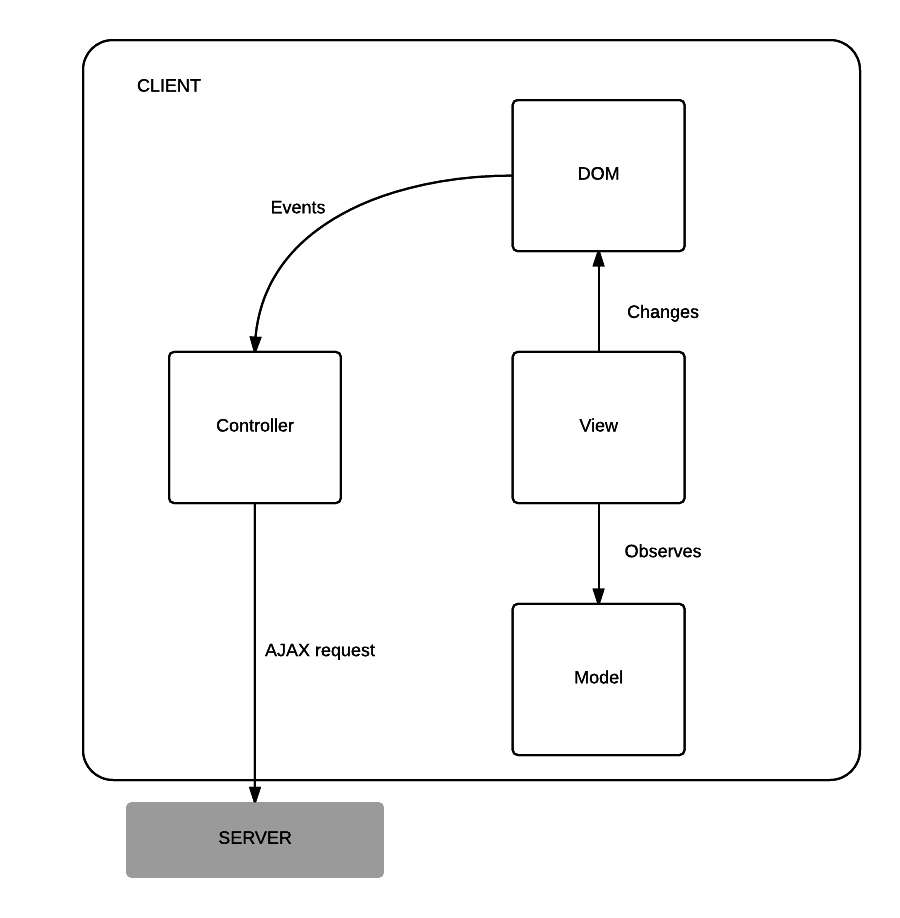
\includegraphics[width=0.75\textwidth]{design/img/webClientArchitecture.png}
	\caption{Client architecture}
	\label{fig:design:ClientArchitecture}
	\end{figure}

	Through the use of \gls{spa} paradigm, our server burden has been simplified since the task of building pages has been transferred to the client which has permitted obtaining rich interactive interfaces that do not need to be reloaded at every request. Moreover, the system has gained better responsiveness because the data transferred rather than being \gls{html} is \gls{json}, known for its compact syntax. Therefore, this solution stands out when compared to the multi-page paradigm that Blaise or SurveyMonkey have in which the entire interface is refreshed on every request \cite{proc:mesbah07} impacting not only over the system performance but also offering poorer user interactivity.


	

	



	

	\section{Implementation Details}\label{sec:cawiSystem:implementation}
			Our \gls{cawi} system solution, clearly separates client and server functionalities to obtain an architecture which offers flexibility and evolvability architectural principles. Section \ref{sec:cawiSystem:serverSide} explains implementation details for the multi-layered server whereas Section \ref{sec:cawiSystem:clientSide} introduces the reader to the three interfaces that give support to survey life-cycle.
		\subsection{The Server Side}\label{sec:cawiSystem:serverSide}
				The server side of our \gls{cawi} system is separated into three layers, i.e. \gls{rest}ful \gls{api}, business layer and data access layer. Section \ref{sec:cawiSystem:restfulImplementation} explains the implementation of \gls{rest} principles through an example that overviews the \gls{http} methods utilised for the collection stage. Regarding the state-transition used for gathering survey data, we have focused on explaining the \gls{rpn} algorithm that evaluates expressions for routing and personalisation constructs on real-time in Section \ref{sec:cawiSystem:rpnEvaluation}.
			\subsubsection{RESTful API}\label{sec:cawiSystem:restfulImplementation}
					The \gls{api} layer used to communicate client and server has been implemented through Jersey, a standard open source framework used to develop RESTful Web Services \footnote{\url{https://jersey.java.net/index.html}} in Java. Throughout this section, a Java class that captures the requirements for the collection stage of surveys (see Listings \ref{code:impl:collectionResource}) will be used to discuss the \gls{api} implemented to communicate the parts. This class defines methods (e.g. public void postToken(...)) to implement functionalities such as resume, forward and backward through an interview. Also, it specifies annotations (e.g. @POST), that permit an easy mapping between a Java class and a web resource.

	\lstinputlisting[caption={Collection resource implementation details},label={code:impl:collectionResource}]{implementation/code/collectionResource.java}

	@Path annotation describes a relative \gls{uri} path to a resource. We have defined this annotation at two levels: at the class level, that permits creating a resource identifier (e.g. \emph{/collection}); and at method level, that specifies a sub resource for a given resource (e.g. \emph{/token\{id\}} that is reachable by clients as \emph{/collection/token\{id\}}). Every request sent to the server requires a survey id for which the interview is conducted (e.g. @PathParam). @Consumes and @Produces define the exchangeable data format used to communicate client and server (e.g. MediaType.APPLICATION\_JSON) for requests and responses respectively. In addition, although it not present on the example provided, every sub resource that consumes or produces survey data and meta data requires a token header containing the interviewee's identifier. Through this header, we have achieved a stateless communication that helps for an easy scaling.

	Our \gls{rest} \gls{api} uses GET, POST and DELETE \gls{http} methods. With @GET annotation it is possible to access to sub resources such as \emph{/surveyinfo}, that retrieves the meta data of a survey like its title, description and data or \emph{/resume}, that gives flexibility for the respondents to choose the right time to continue an interview.

	The modification of sub resources is carried with @POST and @DELETE annotations. @POST, it is used for operations such as moving forward and backward through a questionnaire (e.g. postPrevious(...) or postNext(...)) and for creating a database record for a newer interviewee (e.g. postToken(...)). With respect to the @DELETE, that is used to mark a questionnaire as completed, helps to prevent the modification of survey data by interviewees.
			\subsubsection{The RPN Evaluation}\label{sec:cawiSystem:rpnEvaluation}
					The evaluation of a \gls{rpn} expressions is conducted for every interview that takes place. Every time a variable is updated, the system automatically re-evaluates those \gls{rpn} expressions in which a reference to that variable exists. The algorithm implemented to execute questionnaire expressions in our \gls{cawi} system (see Listings \ref{code:impl:rpn}) only requires two arrays: \emph{expression}, that contains an operand or operator in each position; and \emph{stack}, to simulate push and pop operations through software \cite{web:brown01} for intermediate operations that are carried out while executing an expression.

	\lstinputlisting[caption={The RPN evaluation},label={code:impl:rpn}]{implementation/code/rpn.java}

	The expression array, is read from left to right (e.g. Line 6). If a variable or constant is found (e.g. Lines 7 and 11), it is pushed in the stack. In contrast, the presence of an operator performs one or more operations depending on its type. For binary operations, two operands are popped from the stack whereas for unary operations, only one operand is required. In both cases, if there are still positions to read in the expression array, the intermediate result is pushed in the stack (see Lines 22 and 28). The algorithm terminates when every position of the expression array has been read and its computational complexity cost is linear. Exceptions may be thrown at three different levels:

	\begin{itemize}
		\item At the beginning, in cases where the expression is NULL.
		\item During the loop execution, either because the stack is unexpectedly empty trying to retrieve an operand for unary or binary operation or because the expression contains a token element unknown for the algorithm.
		\item At the end, when the loop has been completed, the stack must have only one element to pop, otherwise a malformed \gls{rpn} expression was passed.
	\end{itemize}
		\subsection{The Client Side}\label{sec:cawiSystem:clientSide}
				The client side of our \gls{cawi} solution organises the interface into three separated applications in order to address the survey life-cycle process. In these interfaces we have used \gls{html}, \gls{css} and JavaScript for structure, presentation and behaviour respectively. The following subsections detail design, collection and other interfaces that have been implemented using the \gls{spa} paradigm. 

	%The client side contains three different interfaces in order to capture the requirements expected for a \gls{cawi} solution. As these has been built separately, multiple developers can focus on different areas in order to add or modify any requirement.

	%The \emph{design} interface contains components to fully describe survey specifications for content (e.g. any type of question and its section associated), routing (e.g. describing any routing with an intuitive expression builder) and personalisation constructs (e.g. randomising and rotating aspects for response sets) according to our \gls{xml} language.

	%The \emph{collection} interface separates the question types in different templates, providing mechanisms to validate data integrity across content aspects and leaving the responsibility to decide the routing to the server. For instance the client interface offers mechanisms to check that any response provided for a question is valid according to a minimum and maximum range specified, i.e. ensuring an open integer response meets the boundaries or the number of choices selected for a multiple question is within a range.

	%The \emph{management} interface encompasses the management, analysis and reporting stages with features such as surveys active, the number of concurrent interviewees and their current location within the questionnaire, real-time charts for every type of question or mechanisms to export survey data and meta data in \gls{csv} format.
			\subsubsection{The Design Interface}\label{sec:cawiSystem:designInterface}
					The interface for designing questionnaires provides high-level visual tools to facilitate the creation of survey features without needing to write any \gls{xml} code. This permits designers, that usually do not have programming skills, to create simple to complex questionnaire specifications. The interface has two modes: one for describing the content and personalisation features; and the other for specifying the questionnaire's routing.

	Figure \ref{fig:impl:designInterface1} represents the look and feel of the authoring tool for questionnaire specifications. Specifically, this screen shot depicts questions INF1, Q1, Q2, Q3 and Q4 from Figure \ref{fig:background:survey} with a top bottom sequence order. At the top, there are two functionalities that are only applicable for a section. These are, \emph{filter} that permits describing a logical expression and \emph{loop} that allows specifying any of the three iteration modes (e.g. range, list and expr\_list explained in the Section \ref{sec:impl:for}). The right side has a toolbox to access to the global variables (e.g. Variable button) as well as to switch to the content screen (e.g. content button). Next to each question there is a button (e.g. wheel) that allows selecting any routing feature. For instance, the example provided describes three skip constructs (e.g. under Q1, Q2 and Q3) where three combo boxes must be specified: the first combo, it is used to select a response from a question given (e.g. response never from Q1); the second requires to choose a binary operator (e.g. IS\_SEL); and the third expects a destination question (e.g. END). In order to avoid circular dependencies, this interface provides mechanisms that prevents questionnaire designers to define skips to questions defined above this construct on the screen.

	\begin{figure}[h]
	\centering
	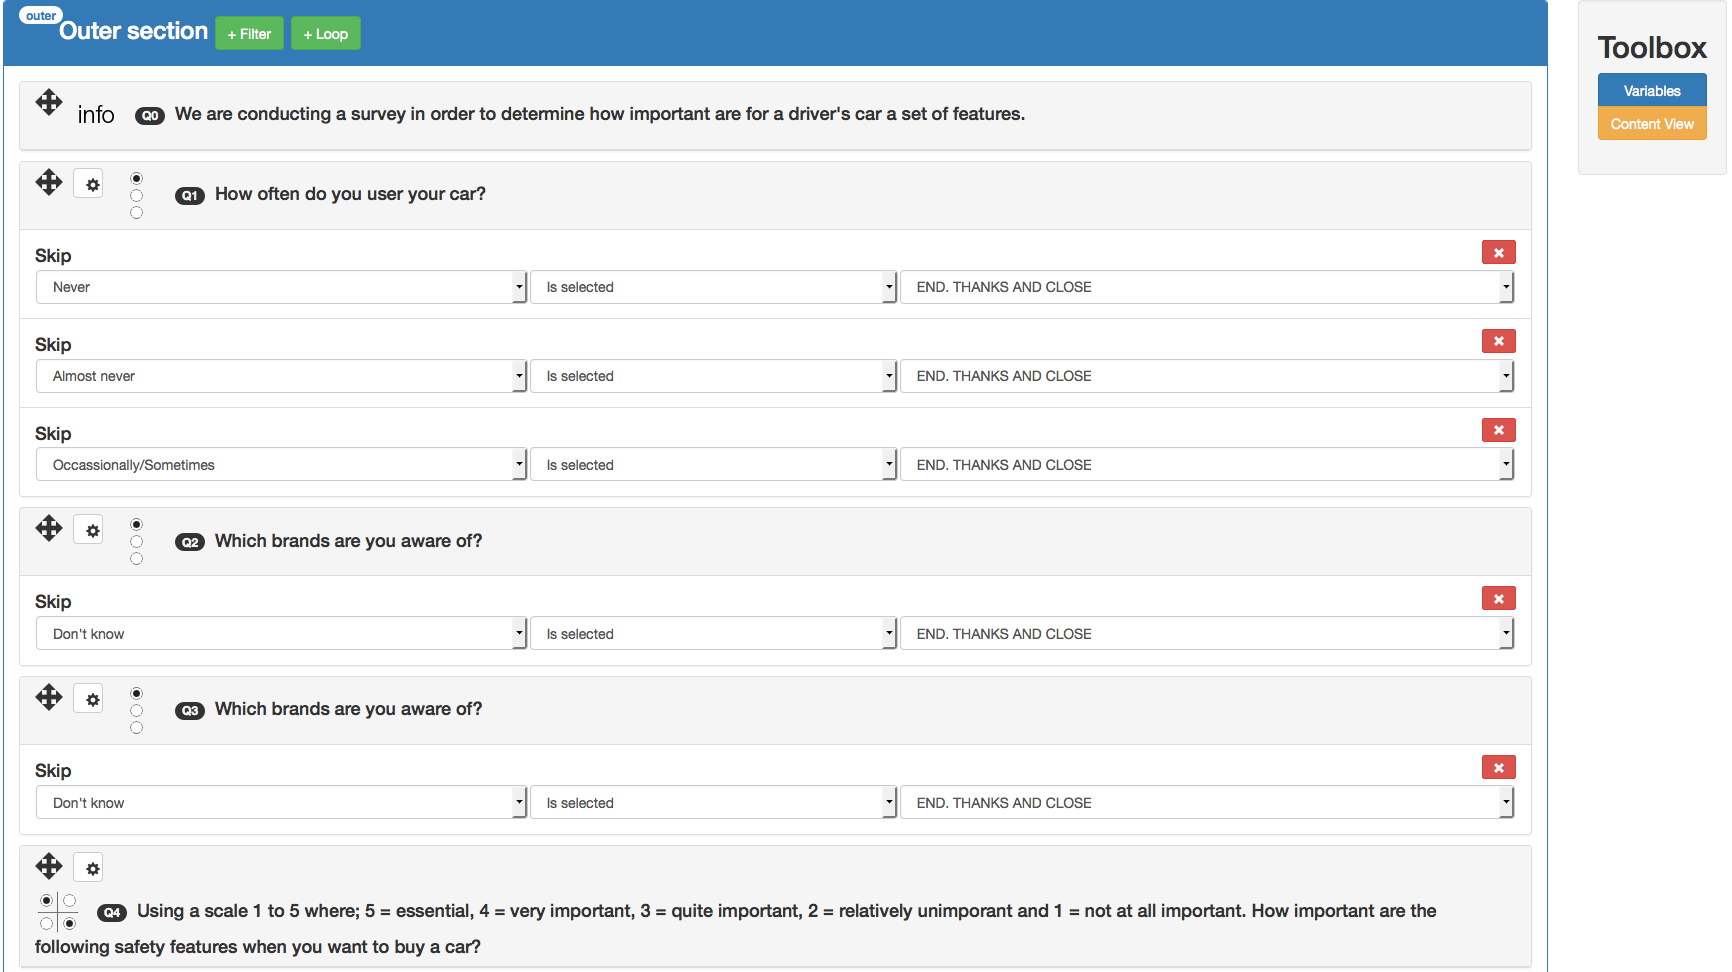
\includegraphics[width=0.90\textwidth]{implementation/img/design_1}
	\caption{Routing design interface}
	\label{fig:impl:designInterface1}
	\end{figure}

	Figure \ref{fig:impl:designInterface2} represents the routing from Q4 till END for the questionnaire Figure \ref{fig:background:survey}. Two constructs are defined; a filter (e.g. over Q5) and an expr\_list loop (e.g. above Q6a). The routing constructs, although are presented in the interface through infix notation mode, are automatically translated to postfix by using the Shunting-yard algorithm \footnote{\url{http://rosettacode.org/wiki/Parsing/Shunting-yard_algorithm\#JavaScript}}. This is mainly due to the fact that \gls{cawiml} only accepts \gls{rpn} expressions for logical and arithmetical operations.

	\begin{figure}[h]
	\centering
	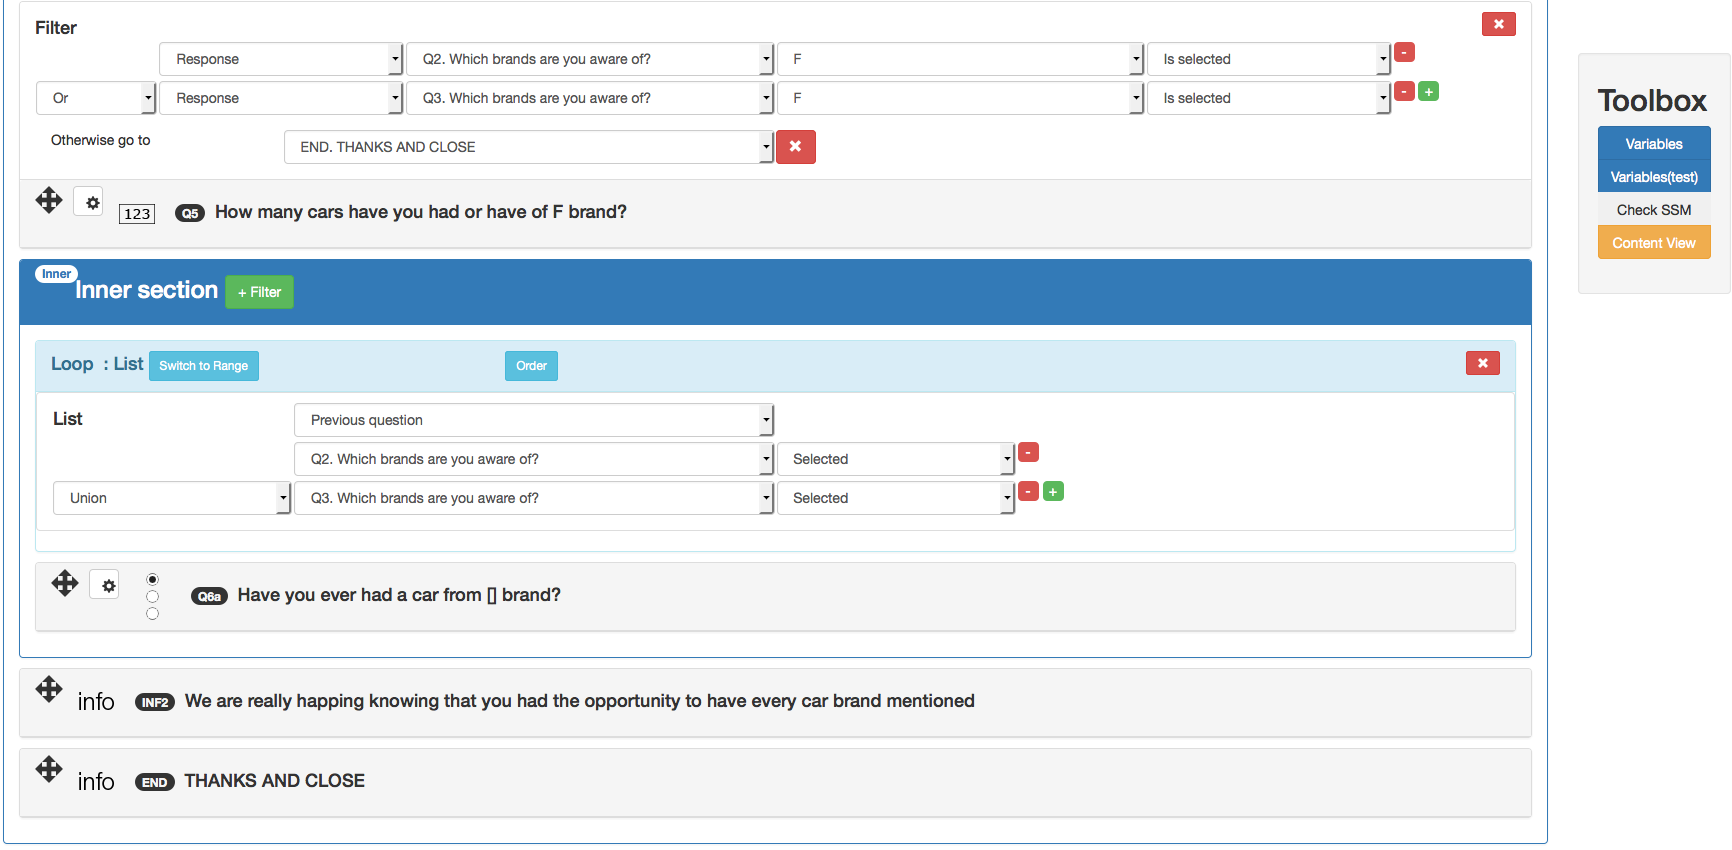
\includegraphics[width=0.90\textwidth]{implementation/img/design_2}
	\caption{Content/Personalisation design interface}
	\label{fig:impl:designInterface2}
	\end{figure}

			\subsubsection{The Collection Interface}
					The interface for collecting survey data separates states such as simple, check, sink or terminate on different template views. The data validation is entirely performed in the client (e.g. checking that the number of chosen responses is between a range, ensuring that every row from a grid question contains at least one response selected or verifying data-types). These validations help to reduce the amount of operations to carry out between server and client. Additionally, as this interface reacts to events immediately, the user experience is greatly improved.

	The stateless restriction from our \gls{rest} architecture requires for each new interview carried out in a browser to persist the interviewee's identifier either by using cookies or through the browser's data storage. Similarly, when the questionnaire is completed, it is the responsibility of the client to delete this persisted id. Every time the navigation is updated, i.e. next or previous action is requested, the server responds with the new state reached and the client redraws the part of the interface that needs to be changed without the need for page reloading.
	
	Figure \ref{fig:impl:collectionInterface} represents an example of an interview demo that was presented at the \gls{xml} Prague conference 2015. %\cite{proc:lloret15}. 
	Firstly the display of the example question provides a language translation option in order to change to other languages. Next, it displays an example of a single question (e.g. Q1) with multiple responses represented through radio buttons. Finally, at the bottom, the navigation options (e.g. previous and next) are presented. Note that the next action appears disabled but it becomes enabled whenever the data entered for a question successfully passes the client validations.

	\begin{figure}[h]
	\centering
	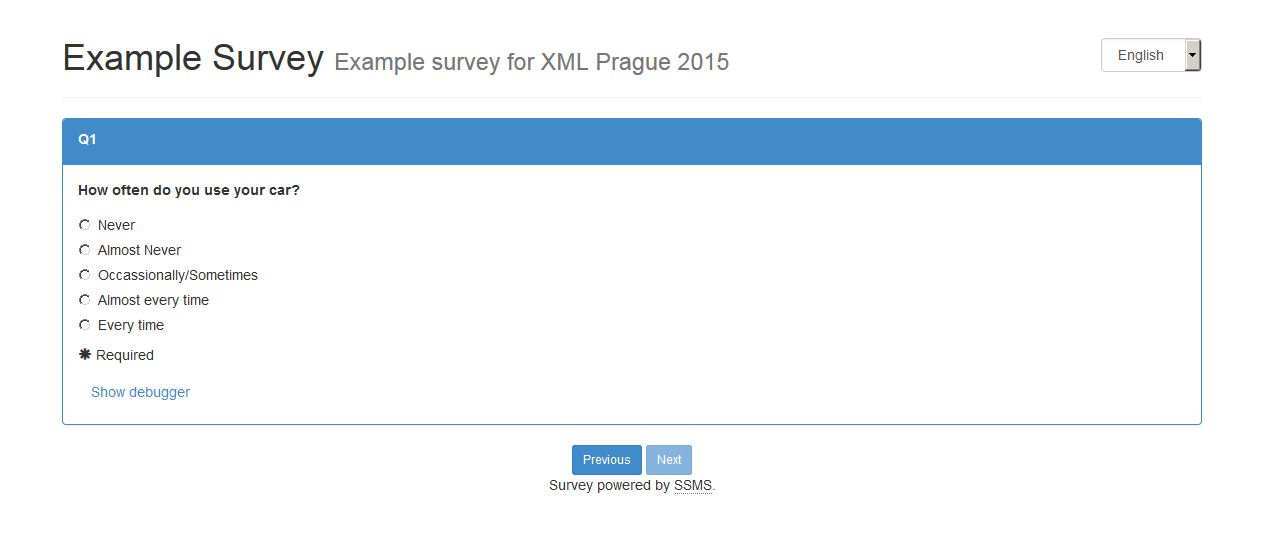
\includegraphics[width=0.90\textwidth]{implementation/img/collection}
	\caption{Collection interface}
	\label{fig:impl:collectionInterface}
	\end{figure}
			\subsubsection{The Management, Analysis and Reporting Interface}
					This interface unifies the management, analysis and reporting stages in one single interface. The most attractive functionalities from this interface is the visualisation of real-time survey responses while interviews are taking place. For that purpose, this interface provides different chart types for each type of question. 

	For instance, Figure \ref{fig:impl:analysisInterface} represents for each interviewee (e.g. y axis), her response to an open-ended question enclosed in one of the six categories (e.g. strong positive, positive, weak positive, weak negative, negative or strong negative) through x axis. This functionality could help to quickly analyse whether or not the responses obtained for an open question match with the survey requirements.

	\begin{figure}[h]
	\centering
	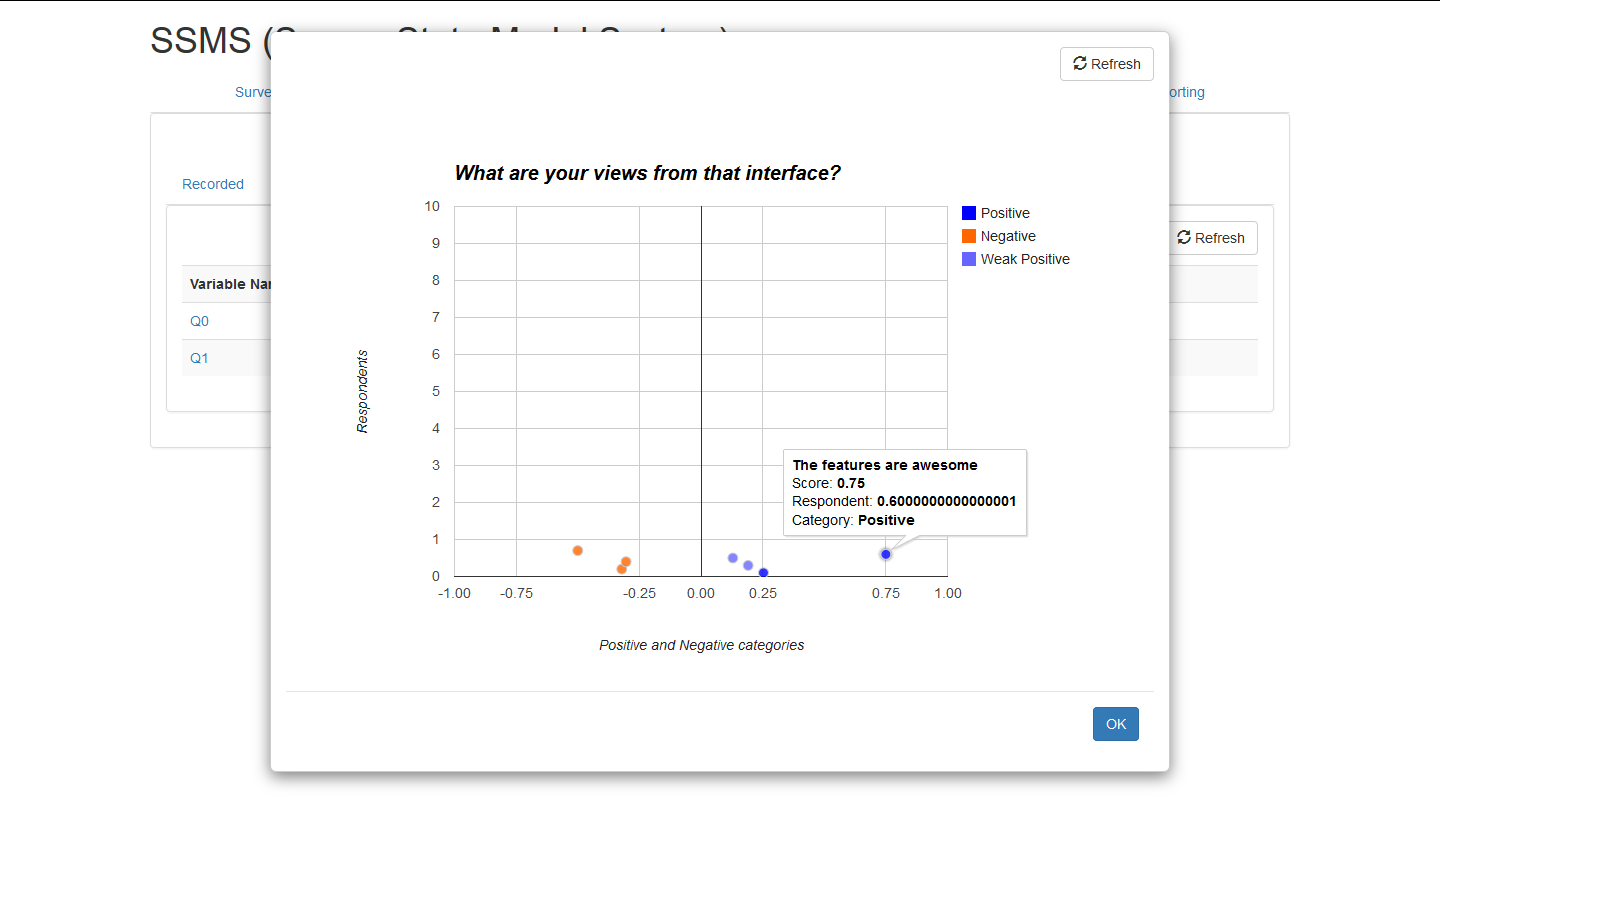
\includegraphics[max size={\textwidth}{\textheight}]{implementation/img/analysis.png}
	\caption{Analysis interface}
	\label{fig:impl:analysisInterface}
	\end{figure}

	\section{Conclusions}\label{sec:cawiSystem:conclusion}
			Our \gls{cawi} system solution for survey life-cycle adopts \gls{rest} constraints to adhere to scalability, simplicity and reliability architectural properties expected for \gls{cawi} systems. Particularly, the \gls{rest} \gls{api}, which conforms to the \gls{http} protocol, has been implemented with the standard reference library for Java. This multi-layered solution is highly portable and uses a \gls{nosql} database solution which permits a more flexible persistence solution when compared to the traditional relational databases.

	The client side, based on the \gls{spa} not only improves the responsiveness of a distributed system but also helps to produce richer interactive interfaces. This paradigm when compared to the multi-page approach that \gls{cawi} systems such as Blaise or SurveyMokey adopt, is more attractive. Particularly, with the choice of AngularJS as the framework for building pages, we have gained a simplified cross browser testing of functionalities, reduced the server burden by transferring interface logics to the client and promoted a parallel development of design and collection interfaces.

	\chapter{Evaluation}\label{ch:evaluation}
			This Chapter presents \gls{cawiml} as an alternative authoring language to specify questionnaires only using standard \gls{xml} schema languages. Particularly, it uses a state-transition paradigm for question's sequence and is intended to facilitate the questionnaire routing logic more adequately than the popular hierarchical model. \gls{rpn}, is the expression formalism utilised for describing routing and personalisation constructs indistinctly.

	The rest of this Chapter is structured as follows: Section \ref{sec:cawiLanguage:stateTransition} introduces the state-transition routing structure. Section \ref{sec:cawiLanguage:rpn} explains the postfix notation mode as the formalism for questionnaire expressions, followed by Section \ref{sec:cawiLanguage:xmlLanguage} that explains our \gls{xml} authoring solution. Finally, \gls{xml} details for content, routing and personalisation constructs expressed in \gls{cawiml} are presented in Section \ref{sec:cawiLanguage:cawiml}.
	\section{XML Language Evaluation}\label{sec:eval:xmlEvaluation}
			In order to test the coverage of questionnaire features through \gls{cawiml} language and to determine typical frequency of constructs, we have randomly chosen a set of fifteen real questionnaires provided by Pexel. Particularly, we have studied the frequency distribution of \gls{cawiml} vocabulary over this sample of surveys. Figure \ref{fig:eval:frequencies} shows the total number of occurrences for each construct sorted by decreasing order of frequency. The bar chart separates the content, routing and personalisation features with purple, green and blue colours respectively. A more detailed view for this dataset, presented in Table \ref{tab:eval:frequencies}, represents frequency of questionnaire constructs separated for each survey. %It was encouraging to us that all the questionnaires in the sample were represented using \gls{ssm} and apart from the check feature, every other construct was included in any of the surveys chosen. 

	\begin{figure}[H]
	\centering
	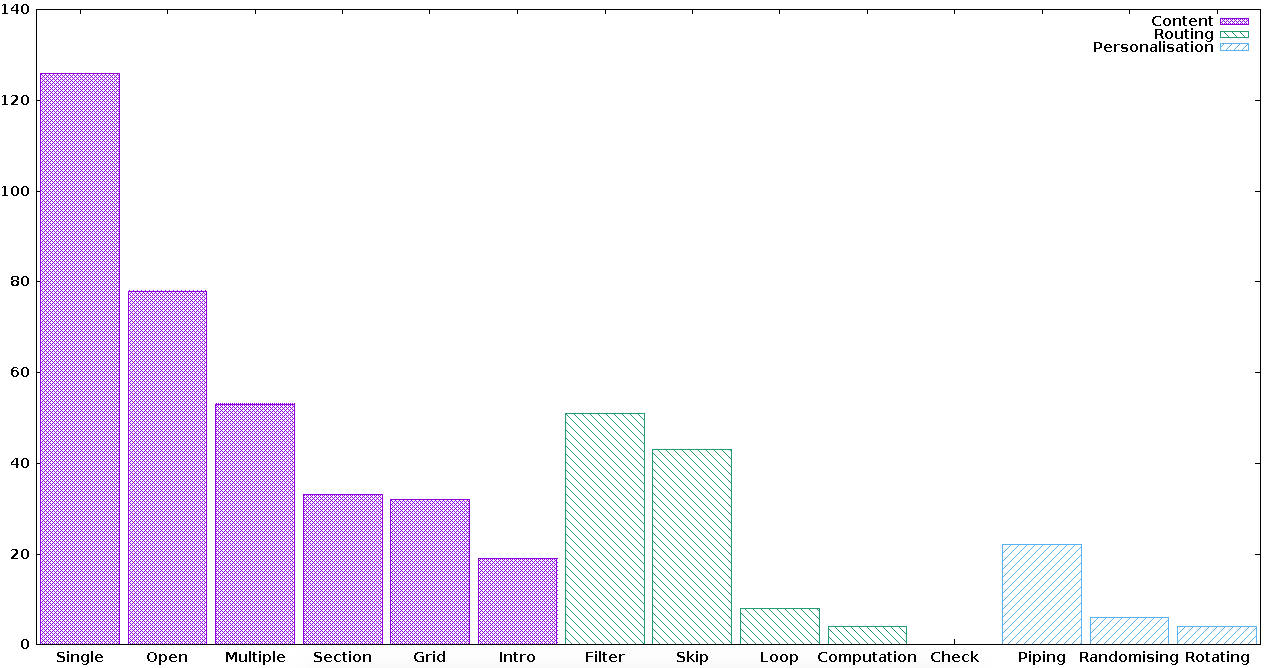
\includegraphics[width=\textwidth]{eval/img/surveyfrequencies.png}
	\caption{Total construct frequencies for fifteen surveys}
	\label{fig:eval:frequencies}
	\end{figure}

	\begin{sidewaystable}
\begin{center}
\begin{tabular}{|c|c|c|c|c|c|c|c|c|c|c|c|c|c|c|c|c|c|}
\hline 
 & Feature & 01 & 02 & 03 & 04 & 05 & 06 & 07 & 08 & 09 & 10 & 11 & 12 & 13 & 14 & 15 & TOTAL\tabularnewline
\hline 
\hline 
\multirow{6}{*}{Content} & Single & 8 & 10 & 7 & 16 & 11 & 8 & 10 & 9 & 2 & 9 & 3 & 9 & 4 & 9 & 11 & 126\tabularnewline
\cline{2-18} 
 & Open-ended & 11 & 1 & 5 & 0 & 11 & 6 & 5 & 1 & 6 & 0 & 12 & 3 & 6 & 9 & 2 & 78\tabularnewline
\cline{2-18} 
 & Multiple & 3 & 0 & 2 & 1 & 1 & 2 & 1 & 6 & 8 & 3 & 8 & 2 & 1 & 7 & 8 & 53\tabularnewline
\cline{2-18} 
 & Section & 1 & 1 & 1 & 7 & 1 & 3 & 2 & 1 & 3 & 5 & 3 & 2 & 1 & 1 & 1 & 33\tabularnewline
\cline{2-18} 
 & Grid & 0 & 0 & 5 & 0 & 1 & 3 & 0 & 1 & 1 & 2 & 0 & 5 & 6 & 7 & 1 & 32\tabularnewline
\cline{2-18} 
 & Intro & 1 & 2 & 1 & 1 & 2 & 1 & 1 & 2 & 1 & 1 & 3 & 0 & 1 & 1 & 1 & 19\tabularnewline
\hline 
\multirow{5}{*}{Routing} & Filter & 1 & 0 & 2 & 0 & 9 & 2 & 0 & 3 & 9 & 3 & 6 & 0 & 5 & 5 & 6 & 51\tabularnewline
\cline{2-18} 
 & Skip logic & 3 & 4 & 1 & 4 & 1 & 5 & 4 & 2 & 2 & 4 & 2 & 4 & 1 & 1 & 5 & 43\tabularnewline
\cline{2-18} 
 & Loop & 0 & 0 & 0 & 0 & 0 & 0 & 0 & 0 & 2 & 0 & 6 & 0 & 0 & 0 & 0 & 8\tabularnewline
\cline{2-18} 
 & Computation & 0 & 0 & 0 & 0 & 0 & 0 & 0 & 0 & 0 & 0 & 0 & 0 & 4 & 0 & 0 & 4\tabularnewline
\cline{2-18} 
 & Check & 0 & 0 & 0 & 0 & 0 & 0 & 0 & 0 & 0 & 0 & 0 & 0 & 0 & 0 & 0 & 0\tabularnewline
\hline 
\multirow{3}{*}{Personalisation} & Piping & 0 & 0 & 3 & 0 & 0 & 0 & 0 & 4 & 9 & 0 & 0 & 0 & 1 & 0 & 5 & 22\tabularnewline
\cline{2-18} 
 & Randomising & 0 & 0 & 0 & 0 & 0 & 0 & 0 & 2 & 1 & 0 & 0 & 0 & 0 & 0 & 3 & 6\tabularnewline
\cline{2-18} 
 & Rotating & 0 & 0 & 0 & 0 & 0 & 0 & 0 & 2 & 0 & 0 & 0 & 0 & 0 & 0 & 2 & 4\tabularnewline
\hline 
\end{tabular}
\caption{Frequency of questionnaire constructs separated by survey}
\label{tab:eval:frequencies}
\end{center}
\end{sidewaystable}


	Firstly, we can confirm that all constructs in our sample of questionnaires were encodable by \gls{cawiml}. Next, in terms of frequency of content, we can observe that single-response questions are most frequent whereas intro constructs were least frequent. Intro question whose purpose is introducing a part of a questionnaire, does not appears once at the beginning instead with each of the sections in the sampled surveys (e.g. questionnaire 04 and 10 with seven and five sections respectively, have only one intro for the entire survey).

	Secondly, for the routing classification, filter construct has obtained the highest number of occurrences, however it does not appear in every questionnaire (e.g. 02, 04, 07, 12). In contrast, the skip feature, although slightly less frequent than filter, is popular amongst the surveys. Therefore, we conclude that skip logic remains an important feature of questionnaires and so should ideally be facilitated by the underlying language of surveys. Computation constructs, become essential when data from one section is needed for another section, but has only been found four times in the questionnaire 13. The absence of check constructs is not surprising since it is a rare feature that tends to appear in less well-designed questionnaires.

	Thirdly, for the personalisation grouping, the three features are presented in the sample tested and piping appears to be the most common construct, specially for populating responses automatically through carry-forward mode. Regarding randomising and rotating constructs, they are less frequent.
	\section{Collection Stage Evaluation}\label{sec:eval:collectionStageEvaluation}
			%We have conducted a load testing experiment to evaluate the performance of the state-transition model and verify whether it works adequately according to a three metrics or not. There are several factors affecting the performance of our RESTful Web service such as the number of concurrent users requesting data, the complexity of the survey and the web server configuration. 

	%This section discusses an approach for testing our model performance by defining a scenario addressed to emulate the interviewee's behaviour when responding a questionnaire. This simulation has been carried out through JMeter \cite{web:jmeter16}, an open source load testing tool which has executed our test plan collecting data for later being analysed.

	\subsection{Methodology}
		In order to evaluate the capacity of our \gls{cawi} system for collecting survey data, we have chosen the stress testing strategy with the following server configuration:
		\begin{itemize}
			\item 2.4 GHz Intel Core i5 CPU,
			\item 1GB RAM dedicated exclusively for the \gls{cawi} system, %the maximum heap size that our Java app can take to allocate the new objects created. 
			\item and a maximum pool size at 100 to satisfy high number of accesses to the database for update/retrieve state-transition objects. %And finally up to 100 cache of database pooling connections to minimise the frequency and number of connections.
		\end{itemize}
		This strategy has been executed with the methodology plan presented in Section \ref{sec:literature:performanceTesting} in which first a questionnaire is selected, second a scenario is designed and thirdly different parameters are varied.
		
		\subsubsection{Survey Choice}

		We have chosen questionnaire 09 (see Appendix \ref{sec:appendix:questionnaires}) since it has an adequate distribution of survey features. Specifically, for the content features, there are: one intro, one single-grid, two single, eight multiple and six open-ended questions. In respect to the routing constructs, there are nine filters, two skip logics and two loops that iterate over a list of responses with sizes nine and thirteen respectively. Regarding the personalisation features, nine pipes are defined either as \emph{text-fill} or \emph{carry forward responses} as well as a randomising construct that changes the element's order for one of the loops.

		\subsubsection{Scenario Design}
		The scenario designed to simulate the gathering of survey data, represented in Algorithm \ref{alg:eval:scenario}, starts with the following statements: first, a new survey instance is created; second, general information of the questionnaire such as title or description is requested; and third, the first state of the survey is called. After that sequence, an iterative process is carried out until the end of the questionnaire is reached.

			\begin{algorithm}
	$\textbf{POST}$ token\;
	$\textbf{GET}$ surveyinfo\;
	$\textbf{GET}$ resume\;
	\While{stateClass $\neq$ Sink AND stateClass $\neq$ Terminate}{
		Random Thinking Time from 500ms to 3000ms\;
		70$\%$ of the iterations\;
			\If{hasNext}{
				Answer question(s) randomly\;
				$\textbf{POST}$ next\;
			}
		30$\%$ of the iterations\;
			\If{hasPrevious}{
				$\textbf{POST}$ previous\;
			}
	}
	$\textbf{DELETE}$ token\;
	\caption{Scenario for stress testing}
	\label{alg:eval:scenario}
	\end{algorithm}

		The loop body firstly executes a random distributed time in order to simulate the amount of time that takes respondents to answer one or more questions and secondly, decides whether executing forward or backward requests for 70\% or 30\% respectively for the total of iterations. We have chosen a higher value for forward requests in order to ensure that every simulated interview is completed. When the forward action is requested, a JavaScript functionality that randomly chooses the response for a question according to its type, is performed. Finally, when the loop is completed, the task of deleting the client token is requested, i.e. a successful response will prevent the virtual respondent to modify her survey responses after that. %EXPLAIN THAT THE JAVASCRIPT EXECUTION IS CARRIED OUT ON THE CLIENT

		\subsubsection{Parameters Varied}

		Two parameters have been considered when the scenario is executed: the \emph{virtual users}, that is the number of concurrent users that are responding to the questionnaire. This constant varies from 50 to 300 by increments of 50; and the \emph{thinking time}, that is randomly distributed from 500 ms to 3000 ms. This parameter has served us to adequately emulate the interviewee's thinking behaviour before responding to a question. 

	\subsection{Metrics}

	We have collected average response time, peak load and error rate for each testing level executed. The \emph{average}, that corresponds to the statistical mean of the population, has been measured in milliseconds. Regarding the \emph{peak load}, that captures the highest response time obtained for all the requests sent, has permitted us to identify bottlenecks in resources. In respect to the \emph{error rate}, that is the percentage of problematic requests from every testing level executed.

	In order to determine the responsiveness of the system we have compared the response times obtained for average and peak load metrics against the following three categories: \emph{100}ms, that is the threshold in which users feel that a system reacts instantaneously to their requests; \emph{1} second, that constitutes the limit for feeling a seamless flow; and \emph{10} seconds, which is the limit to keep user's attention. Any time above that threshold leads to less ideal situations \cite{web:nielsen10}.

	\subsection{Results}

	The results obtained after executing stress testing at different load levels of concurrent users are presented in Table \ref{tab:eval:stressTest}. This table captures for each level the sub resource, number of samples, average response time, minimum response time request, peak load or maximum response time request and the percentage of error. These sub resources correspond to the sub resources exposed to the client in our \gls{cawi} system (see Section \ref{sec:cawiSystem:restfulImplementation}).

	The average response times for each sub resource remained under 100 milliseconds for 50, 100, 150 number of virtual users, i.e. for the interviews carried out at these levels, the respondents will feel that the system reacts instantaneously to their requests. POST token, GET survey info and DELETE token have extended this average response time threshold until 200 and GET survey info has obtained the greatest average performance until 250 simultaneous virtual interviewees. On average, none of the sub resources has exceeded 10 seconds threshold at any level in which the user's attention is difficult to handle. Not surprisingly, POST next and POST previous average response times are significantly higher than the others. In particular, POST next has obtained the highest average response time which is explained due to the fact that one or more \gls{rpn} expressions can be executed when moving from one state to another in the questionnaire's flow.
	
	In respect to the peak load, every request for GET survey info and DELETE token at number of users 50 and 100 has been enclosed under the threshold that the system reacts instantaneously. We have found bottlenecks for POST next at 250 and 300 (e.g. 8095 and 11025 respectively) and for POST previous at 300 (e.g. 11566). We consider that these values above the user's attention threshold are directly related to the number of database connections available when requesting data, i.e. having set up 100 pooling connections has lead the users to wait until a database connection is free for usage.

	Regarding the percentage of errors, it has been encouraging to us that no errors were raised at any configuration level evaluated. This can be explained by the setting of an optimum ramp-up time of 10 users per second entering in the system. This value is sufficiently high to avoid saturating the server with unrealistic requests (e.g. all user at once) at the beginning of each test plan and low enough to prevent any interview to be completed before all the users are concurrently active.

	%-----------------AVG
	%POST token:
	%	Avg under 100 milliseconds for 50,100,150 and 200
	%	Avg less than 1 second for 250 and 300
	%GET surveyinfo:
	%	Avg under 100 milliseconds for 50,100,150,200 and 250
	%	Avg less than 1 second for 300 with a value slightly above system reacts instantaneously
	%GET resume:
	%	Avg under 100 milliseconds for 50,100,150 and 200
	%	Avg less than 1 second for 250 and 300
	%POST next:
	%	Avg under 100 milliseconds for 50,100,150
	%	Avg less than 1 second for 200 and 250
	%	Avg under 10 seconds for 300
	%POST previous:
	%	Avg under 100 milleconds for 50,100,150
	%	Avg less than 1 second for 200 and 250
	%	Avg under 10 seconds for 300
	%DELETE token:
	%	Avg under 100 milliseconds for 50,100,150 and 200
	%	Avg less than 1 second for 250 and 300
	%-----------------PEAK LOAD
	%POST token:
	%	Peak load under 1 second for 50,100,150,200
	%	Peak load less than 10 seconds for 250 and 300 (still good value far from reaching the threshold of loosing user's attention)
	%GET surveyinfo:
	%	Peak load under 100 milliseconds for 50, 150
	%	Peak load under 1 second for 100,200 and 250
	%	Peak load under 10 seconds for 300
	%GET resume:
	%	Peak load under 100 milleconds for 50
	%	Peak load less than 1 second for 100,150,200
	%	Peak load less than 10 seconds for 250 and 300
	%POST next:
	%	Peak load under 1 second for 50, 100
	%	Peak load less than 10 seconds for 150,200
	%	Peak load not acceptable for 250 and 300
	%POST previous:
	%	Peak load under 1 second for 50, 100
	%	Peak load less than 10 seconds for 150,200,250
	%	Peak load not acceptable for 300
	%DELETE token:
	%	Peak load under 100 milliseconds for 50,100
	%	Peak load less than 1 second for 150, 200
	%	Peak load under 10 seconds for 250 and 300

		\begin{table}[H]
	\centering
	\begin{tabular}{|c|c|c|c|c|c|c|}
		\hline 
		\textbf{No. Users} & \textbf{Sub resource} & \textbf{Samples} & \textbf{Avg.} & \textbf{Min} & \textbf{Max} & \textbf{Error \%}\tabularnewline
		\hline 
		\hline 
		\multirow{6}{*}{\textbf{50}} & POST token & 50 & 38 & 19 & 180 & 0.00\%\tabularnewline
		\cline{2-7} 
		 & GET surveyinfo & 50 & 5 & 3 & 10 & 0.00\%\tabularnewline
		\cline{2-7} 
		 & GET resume & 50 & 32 & 20 & 62 & 0.00\%\tabularnewline
		\cline{2-7} 
		 & POST next & 764 & 42 & 12 & 829 & 0.00\%\tabularnewline
		\cline{2-7} 
		 & POST previous & 314 & 46 & 11 & 727 & 0.00\%\tabularnewline
		\cline{2-7} 
		 & DELETE token & 50 & 2 & 2 & 5 & 0.00\%\tabularnewline
		\hline 
		\multirow{6}{*}{\textbf{100}} & POST token & 100 & 30 & 19 & 132 & 0.00\%\tabularnewline
		\cline{2-7} 
		 & GET surveyinfo & 100 & 6 & 3 & 104 & 0.00\%\tabularnewline
		\cline{2-7} 
		 & GET resume & 100 & 28 & 19 & 121 & 0.00\%\tabularnewline
		\cline{2-7} 
		 & POST next & 1563 & 55 & 11 & 330 & 0.00\%\tabularnewline
		\cline{2-7} 
		 & POST previous & 641 & 52 & 12 & 298 & 0.00\%\tabularnewline
		\cline{2-7} 
		 & DELETE token & 100 & 3 & 2 & 18 & 0.00\%\tabularnewline
		\hline 
		\multirow{6}{*}{\textbf{150}} & POST token & 150 & 35 & 18 & 155 & 0.00\%\tabularnewline
		\cline{2-7} 
		 & GET surveyinfo & 150 & 5 & 3 & 45 & 0.00\%\tabularnewline
		\cline{2-7} 
		 & GET resume & 150 & 31 & 19 & 147 & 0.00\%\tabularnewline
		\cline{2-7} 
		 & POST next & 2288 & 89 & 11 & 1089 & 0.00\%\tabularnewline
		\cline{2-7} 
		 & POST previous & 938 & 93 & 12 & 1055 & 0.00\%\tabularnewline
		\cline{2-7} 
		 & DELETE token & 150 & 6 & 2 & 196 & 0.00\%\tabularnewline
		\hline 
		\multirow{6}{*}{\textbf{200}} & POST token & 200 & 54 & 18 & 396 & 0.00\%\tabularnewline
		\cline{2-7} 
		 & GET surveyinfo & 200 & 11 & 3 & 157 & 0.00\%\tabularnewline
		\cline{2-7} 
		 & GET resume & 200 & 55 & 19 & 479 & 0.00\%\tabularnewline
		\cline{2-7} 
		 & POST next & 3146 & 215 & 12 & 3871 & 0.00\%\tabularnewline
		\cline{2-7} 
		 & POST previous & 1288 & 195 & 11 & 3163 & 0.00\%\tabularnewline
		\cline{2-7} 
		 & DELETE token & 200 & 6 & 2 & 218 & 0.00\%\tabularnewline
		\hline 
		\multirow{6}{*}{\textbf{250}} & POST token & 250 & 114 & 18 & 1822 & 0.00\%\tabularnewline
		\cline{2-7} 
		 & GET surveyinfo & 250 & 38 & 3 & 842 & 0.00\%\tabularnewline
		\cline{2-7} 
		 & GET resume & 250 & 168 & 19 & 1623 & 0.00\%\tabularnewline
		\cline{2-7} 
		 & POST next & 4122 & 872 & 12 & 8095 & 0.00\%\tabularnewline
		\cline{2-7} 
		 & POST previous & 1689 & 924 & 11 & 8406 & 0.00\%\tabularnewline
		\cline{2-7} 
		 & DELETE token & 250 & 123 & 1 & 4037 & 0.00\%\tabularnewline
		\hline 
		\multirow{6}{*}{\textbf{300}} & POST token & 300 & 243 & 18 & 2898 & 0.00\%\tabularnewline
		\cline{2-7} 
		 & GET surveyinfo & 300 & 108 & 3 & 3566 & 0.00\%\tabularnewline
		\cline{2-7} 
		 & GET resume & 300 & 504 & 19 & 6133 & 0.00\%\tabularnewline
		\cline{2-7} 
		 & POST next & 4602 & 1737 & 13 & 11025 & 0.00\%\tabularnewline
		\cline{2-7} 
		 & POST previous & 1886 & 1606 & 13 & 11566 & 0.00\%\tabularnewline
		\cline{2-7} 
		 & DELETE token & 300 & 175 & 2 & 3929 & 0.00\%\tabularnewline
		\hline 
	\end{tabular}
	\caption{Stress test results varying No. Users}\label{tab:eval:stressTest}
	\end{table}

	The average response times obtained can be misleading if other aspects such as the standard deviation are not considered. For that purpose, we present in Table \ref{tab:eval:ci} the overall average response time for each configuration level, its standard deviation as well as the confidence value. The standard deviation has resulted higher than its mean at every level, i.e. it indicates that the response times are spread out over the wide range of values. This variety of data can be explained due to the fact that for every interview executed different paths can be taken which result in different durations when moving forward or backward through the questionnaire's flow.

		\begin{table}[H]
	\centering
	\begin{tabular}{|c|c|c|c|c|}
		\hline 
		\textbf{No. Users} & \textbf{Samples} & \textbf{Avg.} & \textbf{Std. Dev.} & \textbf{95\% Confidence}\tabularnewline
		\hline 
		\hline 
		\textbf{50} & 1277 & 40.10893417 & 53.30459906 & 2.923595761\tabularnewline
		\hline 
		\textbf{100} & 2603 & 49.09646426 & 49.82751791 & 1.914168922\tabularnewline
		\hline 
		\textbf{150} & 3825 & 79.93279289 & 98.4293415 & 3.119298604\tabularnewline
		\hline 
		\textbf{200} & 5233 & 182.2417813 & 327.6495887 & 8.877329721\tabularnewline
		\hline 
		\textbf{250} & 6809 & 774.011604 & 1237.580114 & 29.39542518\tabularnewline
		\hline 
		\textbf{300} & 7687 & 1474.736274 & 2013.843128 & 45.01894237\tabularnewline
		\hline 
	\end{tabular}
	\caption{Stress test totals for each configuration level}\label{tab:eval:ci}
	\end{table}

	In order to determine whether or not the average response times obtained are a good estimation of the statistical mean when this scenario is repeated indefinitely, we have also studied the confidence value. As we have collected a large number of independent requests to the server with a finite mean and variance, this parameter permits determining how likely are these overall averages to fluctuate. For instance, for levels 50, 100 and 150, with 95\% confidence, the average response time of the state-transition collection service is 40.11$\pm$2.93, 49.10$\pm$1.92 and 79.94$\pm$3.12 respectively. Similarly, for levels 200, 250, 300, the mean should fluctuate around 182.25$\pm$8.88, 774.02$\pm$29.40 and 1474.74$\pm$45.02 respectively, however at these levels the confidence intervals are significantly higher, which can be directly related with the instability of the system due the high number of simultaneous users connected to the limited resources of the server such as database connections or memory size.

	\section{Conclusions}
			Our \gls{cawi} system solution for survey life-cycle adopts \gls{rest} constraints to adhere to scalability, simplicity and reliability architectural properties expected for \gls{cawi} systems. Particularly, the \gls{rest} \gls{api}, which conforms to the \gls{http} protocol, has been implemented with the standard reference library for Java. This multi-layered solution is highly portable and uses a \gls{nosql} database solution which permits a more flexible persistence solution when compared to the traditional relational databases.

	The client side, based on the \gls{spa} not only improves the responsiveness of a distributed system but also helps to produce richer interactive interfaces. This paradigm when compared to the multi-page approach that \gls{cawi} systems such as Blaise or SurveyMokey adopt, is more attractive. Particularly, with the choice of AngularJS as the framework for building pages, we have gained a simplified cross browser testing of functionalities, reduced the server burden by transferring interface logics to the client and promoted a parallel development of design and collection interfaces.



	Our \gls{cawi} system solution for survey life-cycle adopts \gls{rest} constraints to adhere to scalability, simplicity and reliability architectural properties expected for \gls{cawi} systems. Particularly, the \gls{rest} \gls{api}, which conforms to the \gls{http} protocol, has been implemented with the standard reference library for Java. This multi-layered solution is highly portable and uses a \gls{nosql} database solution which permits a more flexible persistence solution when compared to the traditional relational databases.

	The client side, based on the \gls{spa} not only improves the responsiveness of a distributed system but also helps to produce richer interactive interfaces. This paradigm when compared to the multi-page approach that \gls{cawi} systems such as Blaise or SurveyMokey adopt, is more attractive. Particularly, with the choice of AngularJS as the framework for building pages, we have gained a simplified cross browser testing of functionalities, reduced the server burden by transferring interface logics to the client and promoted a parallel development of design and collection interfaces.

\footnotesize  %NOTE: reduced the size of the text for the bibliography
%NOTE: set the style for the bibliography and display the references used within the document
\bibliographystyle{apalike}
\bibliography{thesis}
\normalsize
\appendix
\chapter{Appendix}\label{ch:appendix}

	\section{Real Questionnaires Sample}\label{sec:appendix:questionnaires}

	The following list represents the fifteen real questionnaires provided by Pexel Research Services that have been implemented in \gls{cawiml}:

	\begin{enumerate}
		\item \url{https://github.com/jollopre/ssm/blob/master/real_surveys/01.xml}
		\item \url{https://github.com/jollopre/ssm/blob/master/real_surveys/02.xml}
		\item \url{https://github.com/jollopre/ssm/blob/master/real_surveys/03.xml}
		\item \url{https://github.com/jollopre/ssm/blob/master/real_surveys/04.xml}
		\item \url{https://github.com/jollopre/ssm/blob/master/real_surveys/05.xml}
		\item \url{https://github.com/jollopre/ssm/blob/master/real_surveys/06.xml}
		\item \url{https://github.com/jollopre/ssm/blob/master/real_surveys/07.xml}
		\item \url{https://github.com/jollopre/ssm/blob/master/real_surveys/08.xml}
		\item \url{https://github.com/jollopre/ssm/blob/master/real_surveys/09.xml}
		\item \url{https://github.com/jollopre/ssm/blob/master/real_surveys/10.xml}
		\item \url{https://github.com/jollopre/ssm/blob/master/real_surveys/11.xml}
		\item \url{https://github.com/jollopre/ssm/blob/master/real_surveys/12.xml}
		\item \url{https://github.com/jollopre/ssm/blob/master/real_surveys/13.xml}
		\item \url{https://github.com/jollopre/ssm/blob/master/real_surveys/14.xml}
		\item \url{https://github.com/jollopre/ssm/blob/master/real_surveys/15.xml}
	\end{enumerate}

	\section{CAWIML Instance}\label{sec:appendix:ssmInstance}

	Listings \ref{code:impl:ssmInstance} captures the paper questionnaire provided in Figure \ref{fig:background:survey}. This instance has been defined using \gls{cawiml} language.
	\lstinputlisting[caption={CAWIML instance},label={code:impl:ssmInstance}]{appendix/code/thesis.xml}






\end{document} %NOTE: END of document, nothing after this point
